% Options for packages loaded elsewhere
\PassOptionsToPackage{unicode}{hyperref}
\PassOptionsToPackage{hyphens}{url}
%
\documentclass[
]{article}
\usepackage{amsmath,amssymb}
\usepackage{iftex}
\ifPDFTeX
  \usepackage[T1]{fontenc}
  \usepackage[utf8]{inputenc}
  \usepackage{textcomp} % provide euro and other symbols
\else % if luatex or xetex
  \usepackage{unicode-math} % this also loads fontspec
  \defaultfontfeatures{Scale=MatchLowercase}
  \defaultfontfeatures[\rmfamily]{Ligatures=TeX,Scale=1}
\fi
\usepackage{lmodern}
\ifPDFTeX\else
  % xetex/luatex font selection
\fi
% Use upquote if available, for straight quotes in verbatim environments
\IfFileExists{upquote.sty}{\usepackage{upquote}}{}
\IfFileExists{microtype.sty}{% use microtype if available
  \usepackage[]{microtype}
  \UseMicrotypeSet[protrusion]{basicmath} % disable protrusion for tt fonts
}{}
\makeatletter
\@ifundefined{KOMAClassName}{% if non-KOMA class
  \IfFileExists{parskip.sty}{%
    \usepackage{parskip}
  }{% else
    \setlength{\parindent}{0pt}
    \setlength{\parskip}{6pt plus 2pt minus 1pt}}
}{% if KOMA class
  \KOMAoptions{parskip=half}}
\makeatother
\usepackage{xcolor}
\usepackage{longtable,booktabs,array}
\usepackage{calc} % for calculating minipage widths
% Correct order of tables after \paragraph or \subparagraph
\usepackage{etoolbox}
\makeatletter
\patchcmd\longtable{\par}{\if@noskipsec\mbox{}\fi\par}{}{}
\makeatother
% Allow footnotes in longtable head/foot
\IfFileExists{footnotehyper.sty}{\usepackage{footnotehyper}}{\usepackage{footnote}}
\makesavenoteenv{longtable}
\usepackage{graphicx}
\makeatletter
\def\maxwidth{\ifdim\Gin@nat@width>\linewidth\linewidth\else\Gin@nat@width\fi}
\def\maxheight{\ifdim\Gin@nat@height>\textheight\textheight\else\Gin@nat@height\fi}
\makeatother
% Scale images if necessary, so that they will not overflow the page
% margins by default, and it is still possible to overwrite the defaults
% using explicit options in \includegraphics[width, height, ...]{}
\setkeys{Gin}{width=\maxwidth,height=\maxheight,keepaspectratio}
% Set default figure placement to htbp
\makeatletter
\def\fps@figure{htbp}
\makeatother
\setlength{\emergencystretch}{3em} % prevent overfull lines
\providecommand{\tightlist}{%
  \setlength{\itemsep}{0pt}\setlength{\parskip}{0pt}}
\setcounter{secnumdepth}{-\maxdimen} % remove section numbering
\ifLuaTeX
  \usepackage{selnolig}  % disable illegal ligatures
\fi
\IfFileExists{bookmark.sty}{\usepackage{bookmark}}{\usepackage{hyperref}}
\IfFileExists{xurl.sty}{\usepackage{xurl}}{} % add URL line breaks if available
\urlstyle{same}
\hypersetup{
  pdftitle={Anytime-valid detection of volatility changes in high-frequency returns with robust truncation},
  pdfauthor={Shreyan Thanki},
  hidelinks,
  pdfcreator={LaTeX via pandoc}}

\title{Anytime-valid detection of volatility changes in high-frequency
returns with robust truncation}
\author{Shreyan Thanki}
\date{Draft, November 2026}

\begin{document}
\maketitle

\hypertarget{abstract}{%
\section{Abstract}\label{abstract}}

We detect volatility changes online in one-minute returns with jumps and
fat tails by two Shiryaev-Roberts betting e-detectors on the squared
return clipped at a multiple of a robust scale. Under the null, with a
known baseline, the average run length to a false alarm is at least
\(A\) and a false alarm within \(m\) steps has probability at most
\(m/A\); a daily restart extends it to every day. No nontrivial
e-process exists for the null that the variance has not fallen, so a
decrease detector needs a bounded statistic, whose clipping level limits
the speed of every deterministic valid rule. A confidence-sequence
baseline gives \(\delta + m/A\) under a tolerance on the conditional
truncated variance; we also bound the delay. Proved monitors keep their
bounds on permuted calm days; most other real-data analyses use a
plug-in baseline without a finite-sample proof. With a
confidence-sequence baseline restarted daily, up alarms followed 8 of 16
FOMC statements of 2024 and 2025 on BTC within six hours, against 11\%
of matched controls, but a pre-registered test on 16 FOMC and CPI
releases of 2026 failed (2 of 16 against 6\%, \(p = 0.25\)), so this
contrast is exploratory. That monitor alarmed on about half of its days:
real days often break its tolerance.

\textbf{Keywords.} Sequential change detection; e-processes; testing by
betting; high-frequency volatility; truncation; jumps; anytime validity.

\hypertarget{introduction}{%
\section{1 Introduction}\label{introduction}}

Volatility in high-frequency markets moves between calm and stressed
regimes, and risk limits, position sizes and model refits should react
when it moves. We ask for an online monitor that reads one-minute
returns, raises an alarm when volatility shifts up or down, and has a
proved limit on false alarms however often it is checked. Two obstacles
make this hard.

\textbf{Jumps and fat tails.} A few extreme returns dominate sums of
squared returns, and a detector built on a Gaussian likelihood reads a
single jump as strong evidence of higher volatility. Jump-robust
estimators address this for a fixed sample: bipower variation
(Barndorff-Nielsen and Shephard 2004), threshold estimators (Mancini
2009), nearest-neighbour truncation (Andersen, Dobrev and Schaumburg
2012), and the kernel quarticity estimator of Bapat (2026), which clips
every return at \(c\) times its median absolute deviation (MAD).

\textbf{Repeated looks.} A fixed-sample test applied at every minute
eventually rejects by chance: in our simulations a 60-step \(z\)-test of
the variance, repeated at every step, raised a false alarm within one
390-step day on 71\% of Gaussian paths. Classical change detection (Page
1954; Shiryaev 1963; Roberts 1966; Lorden 1971; Pollak 1985) controls
the run length to a false alarm but needs the pre-change law.
E-detectors (Shin, Ramdas and Rinaldo 2024) give the same control for
composite, nonparametric nulls, using e-processes built by betting
(Shafer 2021; Ramdas, Grünwald, Vovk and Shafer 2023; Waudby-Smith and
Ramdas 2024).

Robust estimators solve the first problem and betting e-detectors the
second, but these need a statistic whose conditional mean has a meaning
under the null and, to detect a fall in volatility, a bounded one.
Clipping supplies it. The tools we combine are known, and we say where
each comes from; our contributions are three.

\begin{enumerate}
\def\labelenumi{\arabic{enumi}.}
\tightlist
\item
  \textbf{A robust anytime-valid monitor and its limits.} With a known
  baseline, we monitor the clipped squared return under nulls that
  restrict only its conditional mean, prove run-length and
  finite-horizon guarantees, read them over many days, restart the
  monitor to bound every day and bound the effect of a small drift. No
  nontrivial e-process exists for ``the variance has not fallen'', so a
  decrease detector needs a bounded statistic, whose clipping level
  limits the speed of every deterministic valid rule (a rule \(T\) is
  \emph{valid} if \(\mathbb{P}(T \le n) \le n/A\) for every \(n\) and
  every law in the null, with a known baseline; randomised rules obey a
  slightly weaker bound).
\item
  \textbf{An estimated baseline with a clean null.} The plug-in baseline
  keeps its level asymptotically for horizons \(m = o(\sqrt n)\), with
  \(n\) the calibration length (far above 152,100 returns for a 390-step
  day), and can lose it by an unbounded factor otherwise; a
  confidence-sequence baseline gives \(\delta + m/A\) under a tolerance
  on the conditional truncated variance that does not depend on the
  algorithm.
\item
  \textbf{Evidence, including negative results.} A delay theory that
  splits the cost of robustness into three losses, with a delay floor
  for every valid rule; simulations against parametric, robust and
  calibrated classical competitors; null streams built from real
  returns, on which the proved monitors keep their bounds; and real
  series, on which the monitor with a plug-in baseline is about as
  precise as simpler rules matched to its alarm counts and adds little
  to a forecast that sees the last hour.
\end{enumerate}

\textbf{Related work.} Retrospective tests for volatility breaks include
the cumulative sums of squares of Inclán and Tiao (1994) and the
high-frequency test of Bibinger, Jirak and Vetter (2017).\footnote{We
  could not read in full Bibinger, Jirak and Vetter (2017), Chu,
  Stinchcombe and White (1996), Clerico (2025), Dandapanthula and Ramdas
  (2025), Horváth, Hušková, Kokoszka and Steinebach (2004), Horváth,
  Kokoszka and Zhang (2006), Knoblauch, Jewson and Damoulas (2018), Ram
  and Ramdas (2026) and Shekhar and Ramdas (2024), which we checked from
  listings, abstracts and search excerpts, nor Lai (1998) and Mei
  (2008), known to us through secondary sources. What we say about them,
  and every claim of novelty that rests on it, is subject to this
  caveat.} Monitoring with a training sample and asymptotic control of
any false alarm goes back to Chu, Stinchcombe and White (1996) and
covers GARCH parameters (Berkes, Gombay, Horváth and Kokoszka 2004;
Horváth, Trapani and Wang 2025), the unconditional variance (Horváth,
Kokoszka and Zhang 2006) and general parameters (Dette and Gösmann
2020); our guarantee is non-asymptotic and needs no model for the
returns, at the price of a null on a conditional mean. Robust change
detection censors likelihood ratios (Huber 1965), uses least favourable
laws (Unnikrishnan, Veeravalli and Meyn 2009), bounded losses (Fearnhead
and Rigaill 2019) or robust divergences in Bayesian online change-point
detection (Adams and MacKay 2007; Knoblauch, Jewson and Damoulas 2018);
clipping is the betting analogue of censoring. E-value methods for
change detection include sequential estimation (Shekhar and Ramdas
2024), conformal detectors (Vovk et al.~2021) and many streams
(Dandapanthula and Ramdas 2025); Wang and Ramdas (2023) and Mineiro
(2022) give confidence sequences under heavy tails, and e-values have
been applied to risk backtesting (Wang, Wang and Ziegel 2026) and
high-volatility days (Choe and Ramdas 2024). Tartakovsky, Nikiforov and
Basseville (2014) is the standard reference on change detection.
Andersen, Todorov and Zhou (2025) monitor high-frequency prices in real
time for local no-arbitrage violations. To our knowledge, and subject to
the caveat in footnote 1, no published method combines jump-robust
high-frequency volatility measures with anytime-valid change detection
(our search, of November 2026, was not exhaustive).

\textbf{Organisation.} Sections 2 to 5 give the statistic, the
guarantees, estimated baselines and the delay; Sections 6 and 7 report
simulations and an application; Section 8 discusses limitations. The
supplement holds proofs, further results, settings and sources; a
companion note (\texttt{paper/extensions.md}) treats a running
truncation level, restarts, panels of assets, several frequencies and an
adversarial search.

\hypertarget{model-statistic-and-nulls}{%
\section{2 Model, statistic and nulls}\label{model-statistic-and-nulls}}

\textbf{Returns and information.} Let \(r_t\) be the one-minute log
return ending at minute \(t\). Monitoring starts after a calibration
window \(r_{-n+1}, \dots, r_0\), and \(\mathcal{F}_t\) is the
information up to time \(t\): the returns and, when returns can be
missing, the indicators of which were observed. A quantity is
\emph{predictable} if its value used at time \(t\) is
\(\mathcal{F}_{t-1}\)-measurable. Everything the monitor uses
(truncation level, baseline, bets, intraday profile) must be
predictable.

\textbf{The statistic.} Bapat (2026) clips returns at \(c = 3\) times
the MAD of the whole sample before forming a kernel estimate of local
quarticity. We keep the clipping and change three things. We use the
scaled MAD about zero,
\(\hat s = 1.4826\,\mathrm{median}_i \lvert r_i\rvert\) (the median of
one-minute returns is 0 in all our data sets), so that with Gaussian
returns the cut-off \(\tau = c\,\hat s\) sits at \(c\) standard
deviations rather than at \(0.6745\,c\); \(\hat s\) and \(\tau\) come
from the calibration window, so \(\tau\) is
\(\mathcal{F}_0\)-measurable; and we monitor \[
X_t = \min(r_t^2, \tau^2) \in [0, \tau^2],
\] the summand of truncated realised variance, rather than a fourth
power. Supplement S1.8 compares fourth powers and gives the predictable
rule used when most returns of a calibration window are zero.

\textbf{Truncated moments.} For \(Z \sim N(0,1)\) with density
\(\varphi\) and distribution function \(\Phi\), and a cut-off \(a > 0\),
let \[
\kappa_2(a) = \mathbb{E}[\min(Z^2, a^2)] = 2\Phi(a) - 1 - 2a\varphi(a) + 2a^2(1 - \Phi(a)).
\] For \(c = 3\) and the scaled MAD (\(a = 3\)), 0.27\% of Gaussian
returns are clipped and \(\kappa_2 = 0.995\); with the raw MAD
(\(a = 2.023\)), 4.3\% are clipped and \(\kappa_2 = 0.925\). For
Gaussian returns with standard deviation \(\sigma_0\) the mean of
\(X_t\) is \(\kappa_2(c)\sigma_0^2\), and \(\tau^2\) divided by it is
\(c^2/\kappa_2(c)\), which equals 9.045 for \(c = 3\).

\textbf{Intraday seasonality and missing returns.} Each return is
divided by a predictable intraday profile (for crypto, the median of
\(\lvert r\rvert\) at the same minute over the previous 20 days,
smoothed across neighbouring minutes; Andersen and Bollerslev 1997;
Boudt, Croux and Laurent 2011), treated as known; errors in it violate
the null. Missing returns, and the first return after a gap, are
skipped, not set to zero; validity then needs that, given the past,
whether \(r_t\) is observed carries no information about its size.
Horizons \(m\) count monitored steps.

\textbf{Nulls.} Let \(\mu_t = \mathbb{E}[X_t \mid \mathcal{F}_{t-1}]\)
be the conditional truncated variance and \(m_0 > 0\) a baseline. For a
band \(b \in [0, 1)\) fixed in advance, the nulls are \[
H_0^{\uparrow}:\ \mu_t \le (1+b)\,m_0 \ \text{ for all } t \ge 1, \qquad H_0^{\downarrow}:\ \mu_t \ge (1-b)\,m_0 \ \text{ for all } t \ge 1.
\] They restrict one conditional moment and allow any return law, any
jumps and any dependence that keeps that moment on the null side at
every step. Persistent volatility clustering and price-level
microstructure noise both move it, even when the unconditional variance
is constant (Section 6.4).

\textbf{Lemma 1 (volatility meaning).} Suppose
\(r_t = \sigma_t \varepsilon_t\), where \(\sigma_t > 0\) is
\(\mathcal{F}_{t-1}\)-measurable and \(\varepsilon_t\) is independent of
\(\mathcal{F}_{t-1}\) with a law \(G\) that does not depend on \(t\).
Let \(\tau\) be \(\mathcal{F}_0\)-measurable and
\(g_\tau(s) = \mathbb{E}_G[\min(s^2\varepsilon^2, \tau^2)]\). Then
\(\mu_t = g_\tau(\sigma_t)\), and \(g_\tau\) is nondecreasing on
\((0, \infty)\); it is strictly increasing on every interval of values
\(s\) with \(G(0 < \lvert\varepsilon\rvert < \tau/s) > 0\). Hence, with
\(m_0 = g_\tau(\sigma_0)\) and \(b = 0\), \(H_0^{\uparrow}\) holds
whenever \(\sigma_t \le \sigma_0\) for all \(t\), and
\(H_0^{\downarrow}\) whenever \(\sigma_t \ge \sigma_0\) for all \(t\).

The proof is in Supplement S1.5; only the size of the change in
\(\mu_t\) for a given change in \(\sigma_t\) depends on \(G\). Three
caveats follow. A change in tail shape at fixed \(\sigma_t\) also moves
\(\mu_t\): with \(c = 3\), Student \(t\) innovations at the same
variance lower it, which reads as a decrease. With a contemporaneous
leverage effect \(\mu_t\) need not be monotone in \(\sigma_t\). And
returns of prices rounded to a tick are not of the form
\(\sigma_t\varepsilon_t\) with a fixed \(G\), so for them the null is a
statement about \(\mu_t\) only.

\hypertarget{validity}{%
\section{3 Validity}\label{validity}}

\hypertarget{betting-e-detectors-and-the-false-alarm-guarantees}{%
\subsection{3.1 Betting e-detectors and the false alarm
guarantees}\label{betting-e-detectors-and-the-false-alarm-guarantees}}

Write \(m^{\uparrow} = (1+b)m_0\), \(m^{\downarrow} = (1-b)m_0\) and
\(B = \tau^2/m^{\downarrow} > 1\), and let \(Y_t = X_t/m^{\uparrow}\) on
the increase side and \(Y_t = X_t/m^{\downarrow} \in [0, B]\) on the
decrease side. With a predictable bet \(\lambda_t\) define the betting
factors \[
f_t^{\uparrow} = 1 + \lambda_t (Y_t - 1), \ \ \lambda_t \in [0, 1), \qquad f_t^{\downarrow} = 1 + \lambda_t (1 - Y_t), \ \ \lambda_t \in \big[0, 1/(B-1)\big).
\] Both are positive, since \(Y_t \ge 0\) and, on the decrease side,
\(Y_t \le B\). Under the corresponding null,
\(\mathbb{E}[f_t \mid \mathcal{F}_{t-1}] \le 1\), so for every start
time \(j\) the wealth \(L_t^{(j)} = \prod_{s=j}^{t} f_s\) (with
\(L_{j-1}^{(j)} = 1\)) is a nonnegative supermartingale with initial
value 1, a \emph{test supermartingale}.

\textbf{Definition (Shiryaev-Roberts e-detector).} Fix bets
\(\lambda_1, \dots, \lambda_K\) in the admissible range and weights
\(w_k > 0\) with \(\sum_k w_k = 1\). For each \(k\) let
\(M_t^{(k)} = f_t^{(k)}(M_{t-1}^{(k)} + 1)\) with \(M_0^{(k)} = 0\), so
that \(M_t^{(k)} = \sum_{j=1}^{t} \prod_{s=j}^{t} f_s^{(k)}\) is the
total wealth of bettors who start at every time \(j \le t\). Let
\(M_t = \sum_k w_k M_t^{(k)}\) and raise an alarm at
\(T_A = \inf\lbrace t \ge 1 : M_t \ge A \rbrace\).

The default grids, used throughout, are
\(\lambda \in \lbrace 0.02, 0.05, 0.1, 0.2, 0.35, 0.5 \rbrace\) for
increases and
\(\lambda/\lambda_{\max} \in \lbrace 0.1, 0.25, 0.5, 0.75, 0.95 \rbrace\)
with \(\lambda_{\max} = 1/(B-1)\) for decreases, with equal weights. An
update costs \(O(K)\) operations.

\textbf{Lemma 2.} Under the null,
\(\mathbb{E}[M_t \mid \mathcal{F}_{t-1}] \le M_{t-1} + 1\) for every
\(t \ge 1\), so \(M_t - t\) is a supermartingale. The same holds for any
predictable bets and for any average of such statistics with fixed
weights.

\emph{Proof.}
\(\mathbb{E}[M_t^{(k)} \mid \mathcal{F}_{t-1}] = \mathbb{E}[f_t^{(k)} \mid \mathcal{F}_{t-1}](M_{t-1}^{(k)} + 1) \le M_{t-1}^{(k)} + 1\);
average over \(k\). \(\square\)

\textbf{Theorem 3 (average run length).} Under the null,
\(\mathbb{E}[T_A] \ge A\) for every \(A > 0\).

Theorem 3 is the run-length guarantee of e-detectors (Shin, Ramdas and
Rinaldo 2024); Supplement S1.5 gives the proof with its conditions
explicit. A practitioner usually needs a statement for a finite horizon.

\textbf{Theorem 4 (false alarm within a horizon).} Under the null,
\(\mathbb{P}(T_A \le m) \le m/A\) for every integer \(m \ge 1\).

\emph{Proof.} For \(0 \le t \le m\) let \(S_t = M_t + (m - t)\). By
Lemma 2, \(S\) is a nonnegative supermartingale on
\(\lbrace 0, \dots, m \rbrace\) with \(S_0 = m\). Ville's inequality
gives \(\mathbb{P}(\max_{t \le m} S_t \ge A) \le m/A\), and
\(M_t \ge A\) implies \(S_t \ge A\). \(\square\)

The argument is elementary and not new, but its reading over many days
needs care. With \(A = 7800\) for a 390-step trading day, or
\(A = 28{,}800\) for a 1440-minute crypto day, Theorem 4 bounds by 5\%
the probability of a false alarm within the first day after the
statistics start at 0 (at the start of monitoring or after a
recalibration), not on a later day (Proposition 7). The CUSUM-type
statistic \(C_t = f_t \max(C_{t-1}, 1)\) satisfies \(C_t \le M_t\) and
inherits Theorems 3 and 4.

\textbf{Proposition 5 (two-sided monitoring).} Under the two-sided null
\((1-b)m_0 \le \mu_t \le (1+b)m_0\) for all \(t\), the average
\(\bar M_t = (M_t^{\uparrow} + M_t^{\downarrow})/2\) of the two side
statistics satisfies Lemma 2. Hence the rule that alarms at the first
\(t\) with \(\bar M_t \ge A\), and the rule that alarms at the first
\(t\) with \(\max(M_t^{\uparrow}, M_t^{\downarrow}) \ge 2A\), both
satisfy Theorems 3 and 4.

Proposition 5 follows from Lemma 2 (Supplement S1.5). All our
experiments use the maximum rule, which names the direction of an alarm
by the side that crossed; the average rule is never later, but the gain
is small.

\textbf{Corollary 6 (restarts after alarms).} Suppose the monitor
recalibrates after every alarm, with a truncation level \(\tau_q\) and
baseline \(m_0^{(q)}\) for segment \(q\) that are known at the start of
the segment, and that the two-sided null holds in every segment relative
to its own baseline. Let \(N_m\) be the number of alarms within the
first \(m\) monitored steps (calibration steps are not counted). Then
\(\mathbb{E}[N_m] \le m/A\).

The proof and a simulation check are in Supplement S1.1. With \(b = 0\)
the hypothesis asks that each segment's baseline equal the true
conditional mean of its statistic, which no estimated baseline achieves;
Corollary 18 covers a confidence-sequence baseline.

\textbf{Later days.} Let day \(d\) be the steps
\((d-1)m + 1, \dots, dm\), and let \(\bar M_t\) be the statistic of the
alarm rule: \(M_t\) for one side at level \(A\), or the average of
Proposition 5 for the two-sided rule.

\textbf{Proposition 7 (after the first day).} Under the null, with a
known baseline and \(b = 0\), for every \(s \ge 0\) and \(m \ge 1\),
\(\mathbb{P}(\text{an alarm at one of } s + 1, \dots, s + m \mid \mathcal{F}_s) \le \min\lbrace 1, (\bar M_s + m)/A\rbrace\),
so a false alarm on day \(d\) has probability at most \(\min(1, dm/A)\).
No bound below 1 holds for all days, even over i.i.d. laws: the law with
\(\lvert r_t\rvert = \sqrt{m_0}\), under which \(Y_t = 1\), is in the
two-sided null and makes every Shiryaev-Roberts statistic equal to
\(t\), so the two-sided rule alarms with certainty at step
\(\lceil 2A\rceil\), on day 40 for \((m, A) = (390, 7800)\) and for
\((1440, 28{,}800)\).

By Lemma 2 the statistic enters day \(d\) with up to \((d-1)m\) in
expectation. With 390-step days and i.i.d. Gaussian returns the
probability of a first false alarm on day \(d\), given none before, rose
from 0.98\% on day 1 to 4.7\% on average over days 11 to 20, and after
long stretches with \(Y_t = 1\) it was far higher for a Gaussian day
(Supplement S1.7). Over many days the plain detector's guarantee is thus
an expected count (Corollary 6); it meets the window-limited criterion
of Lai (1998) only for the first window, and Mei (2008) shows why the
run length alone can mislead (footnote 1).

\textbf{A bound for every day.} Let \(0 = b_0 < b_1 < \dots\) be
stopping times with \(b_{i+1} - b_i \le m\) (in practice the day
starts), and at each \(b_i\) scale each side's statistics down by a
common factor so that the side's average is at most \(\iota \ge 0\);
\(\iota = 0\) is a restart at 0.

\textbf{Theorem 8 (restart at every day boundary).} With a known
baseline and under the null of Theorem 4, or of Proposition 5 for the
two-sided rule,
\(\mathbb{P}(\text{an alarm in } (b_i, b_{i+1}] \mid \mathcal{F}_{b_i}) \le \min\lbrace 1, (m + \iota)/A\rbrace\)
almost surely for every \(i\). If the statistics also restart after
every alarm, the expected number of alarms in \((b_i, b_{i+1}]\) given
\(\mathcal{F}_{b_i}\) is at most \((m + \iota)/A\).

With \(\iota = 0\) and \(A = m/\alpha\), the false alarm probability,
the expected number of false alarms and the hazard of every day are at
most \(\alpha\) given the past (since
\(\lbrace T_A > b_i\rbrace \in \mathcal{F}_{b_i}\)), and a window of
\(m\) steps that starts in day \(i\), whatever boundaries it crosses,
has an alarm with probability at most \((2m + \iota - 1)/A\) given
\(\mathcal{F}_{b_i}\), though not given the past at its start
(Supplement S1.7). With the confidence-sequence baseline the restart
gives \(\delta + m/A\) per day only marginally, while the tolerance
holds during that day (Corollary S14); with the plug-in nothing per day
is proved. The price is delay for a change late in a day (Proposition
S6). A CUSUM-type statistic bounds the unconditional probability of an
alarm in every window, but only for exchangeable returns, fixed bets and
a known baseline, and was slower (Theorem S7, Proposition S8; Supplement
S1.7).

\hypertarget{a-small-drift-of-the-conditional-mean}{%
\subsection{3.2 A small drift of the conditional
mean}\label{a-small-drift-of-the-conditional-mean}}

The guarantees need the null at every step. The next result says what is
left when it holds only up to a drift. Write \(\lambda_k^{\uparrow}\)
(\(w_k^{\uparrow}\)) for the increase bets (weights) and
\(\lambda_l^{\downarrow}\) (\(w_l^{\downarrow}\)) for the decrease bets,
and for \(x \ge 0\) and an integer \(m \ge 1\) let \[
\Upsilon_m(x) = \frac{(1 + x)\big((1 + x)^m - 1\big)}{m x}, \qquad \Upsilon_m(0) = 1,
\] the average of \((1+x)^j\) over \(j = 1, \dots, m\).

\textbf{Theorem 9 (drift of the conditional mean).} Suppose that
\(\mu_t \le (1 + \xi^{\uparrow})\,m^{\uparrow}\) and
\(\mu_t \ge (1 - \xi^{\downarrow})\,m^{\downarrow}\) for all \(t\), with
constants \(\xi^{\uparrow}, \xi^{\downarrow} \ge 0\) known at time 0.
Then for the two-sided rule of Proposition 5 with the maximum and every
\(m \ge 1\), \[
\mathbb{P}(T_A \le m) \le \min\Big\lbrace 1,\ \frac{m}{A}\,\Gamma_m(\xi^{\uparrow}, \xi^{\downarrow}) \Big\rbrace, \qquad
\Gamma_m(\xi^{\uparrow}, \xi^{\downarrow}) = \frac12\Big[\sum_k w_k^{\uparrow}\,\Upsilon_m(\lambda_k^{\uparrow}\xi^{\uparrow}) + \sum_l w_l^{\downarrow}\,\Upsilon_m(\lambda_l^{\downarrow}\xi^{\downarrow})\Big].
\] With \(\xi^{\uparrow} = \xi^{\downarrow} = 0\) this is Theorem 4.

The proof is in Supplement S1.2. For the default detector (\(c = 3\),
\(b = 0\), \(A = 7800\)), \(\Gamma_m\) is close to 1 while the drift
times the horizon is small (5.80\% instead of 5\% at one day for a drift
of 0.5\% on both sides) and then compounds: the one-day bound doubles at
a drift of 1.63\%, and a drift of 0.5\% exhausts the five-day bound
(Table S1). A drift that alternates costs far less, but no bound in the
mean drift alone exists (Supplement S1.3). So the null holds
approximately when the conditional mean stays within a few tenths of a
percent of the baseline over a day, or when a band \(b\) absorbs the
drift.

\hypertarget{why-a-decrease-detector-needs-a-bounded-statistic}{%
\subsection{3.3 Why a decrease detector needs a bounded
statistic}\label{why-a-decrease-detector-needs-a-bounded-statistic}}

\textbf{Proposition 10.} Let \(\mathcal{N}_\infty\) be the set of all
probability laws on \([0, \infty)\) with mean at least 1. If
\(E: [0, \infty) \to [0, \infty]\) is measurable and
\(\mathbb{E}_P[E(Y)] \le 1\) for every \(P \in \mathcal{N}_\infty\),
then \(E(y) \le 1\) for every \(y \ge 0\).

\textbf{Corollary 11 (no e-process for ``the variance has not
fallen'').} Let \(\mathcal{P}^{\downarrow}\) be the set of laws of real
sequences \((r_t)_{t \ge 1}\) with
\(\mathbb{E}[r_t^2 \mid r_1, \dots, r_{t-1}] \ge m_0\) for every \(t\).
If \(W_t = W_t(r_1, \dots, r_t) \ge 0\) satisfies
\(\mathbb{E}_P[W_t] \le 1\) for every \(P \in \mathcal{P}^{\downarrow}\)
and every fixed \(t\), then \(W_t \le 1\) for every \(t\) and every
path. Consequently a Shiryaev-Roberts statistic built from such
processes started at each time satisfies \(M_t \le t\) on every path,
and cannot alarm before time \(A\), whatever the data.

The proof (Supplement S1.4) builds, for any path, a law in
\(\mathcal{P}^{\downarrow}\) that follows the path with probability
close to 1, a one-sided relative of the result of Bahadur and Savage
(1956). The increase null admits nontrivial e-variables such as
\(E(y) = y\), so an increase detector works on raw squared returns, but
no nonparametric e-test detects a fall in the variance itself. For a
statistic in \([0, B]\) the null ``mean at least 1'' admits the bets
\(1 + \lambda(1 - y)\), \(\lambda \in [0, 1/(B-1)]\), and up to
domination only these (Lemma 20). Truncation is one bounded functional
with a volatility meaning (Lemma 1); ranks are another (Section 6.5).
Its price is a speed limit: one step multiplies a decrease bet's wealth
by at most \(B/(B-1)\) (Corollary 22); for increases, clipping bounds
the effect of one jump.

\textbf{Every valid rule.} The next result bounds every valid rule
(Section 1), with a known baseline and \(b = 0\). Let \(\pi(y)\) be the
largest probability that a law on \([0, B]\) in the null can put on the
value \(y\): under the decrease null (conditional mean at least 1),
\(\pi(y) = (B-1)/(B-y)\) for \(y < 1\) and 1 otherwise; under the
increase null (at most 1), \(\pi(y) = 1/y\) for \(y > 1\) and 1
otherwise; under the two-sided null (equal to 1), the product of the
two. For a path \(y = (y_1, y_2, \dots)\) of \(Y_t = X_t/m_0\) let
\(\Pi_n(y) = \prod_{s \le n} 1/\pi(y_s)\).

\textbf{Theorem 12 (pathwise floor).} Let \(T\) be a stopping rule with
\(\mathbb{P}(T \le n) \le n/A\) for every \(n\) and every law of
\((Y_t)\) on \([0, B]\) in one of the three nulls, with a known baseline
and \(b = 0\). (a) If \(T\) is deterministic, it stops at step \(n\) on
the path \(y\) only if \(\Pi_n(y) \ge A/n\). (b) If \(T\) is randomised
independently of the data,
\(\mathbb{P}(T \le n \mid y) \le (n/A)\,\Pi_n(y)\). (c) For every path
\(y\) and every \(n\) with \(\Pi_n(y) \ge A/n\), some deterministic rule
with the same guarantee stops at \(n\) on \(y\).

\textbf{Corollary 13.} (a) For the decrease null on \([0, \infty)\),
that is without truncation, no deterministic rule valid at levels
\(n/A\) alarms before step \(A\), on any path. (b) On a complete
collapse, \(y_s = 0\) for every \(s\), every deterministic rule valid at
levels \(n/A\) for the decrease or the two-sided null needs at least
\(\min\lbrace n : n \log(B/(B-1)) \ge \log(A/n)\rbrace\) steps: 45 at
\(c = 3\) and \(A = 7800\). A randomised valid rule alarms by step \(n\)
on that path with probability at most \(\min(1, n\Pi_n/A)\), which is
0.98 at step 44; this cap alone gives a mean delay there of at least
37.8, and a linear programme that imposes validity at every \(n\) gives
43.4 (Supplement S1.6).

The proof (Supplement S1.6) places at each step the two-point null law
that gives \(y_s\) its largest probability; under this product law the
path has probability \(1/\Pi_n(y)\), so a rule that stops there spends
at least that much of its budget \(n/A\). The laws can be placed on the
returns, so the floor binds rules that see \(r_t\), and part (a) extends
Corollary 11 to every deterministic procedure. We claim no priority for
this elementary argument; Clerico (2025) shows a related optimality of
betting for a bounded mean (footnote 1).

\hypertarget{estimated-baseline}{%
\section{4 Estimated baseline}\label{estimated-baseline}}

The guarantees above assume that the baseline \(m_0\) and the level
\(\tau\) are fixed in advance, or at least that the null holds with
whatever values the monitor uses. In practice both are estimated from a
calibration window.

\hypertarget{the-plug-in-baseline}{%
\subsection{4.1 The plug-in baseline}\label{the-plug-in-baseline}}

The \emph{plug-in} baseline \(\hat m\) is the mean of \(X\) over the
window, with \(\tau\) from the same window. With 390 calibration steps
its one-day false alarm rate on the increase side was 4.58\% to 5.10\%
across Gaussian, Student \(t_3\) and jump returns, against 1.62\% to
1.75\% with the true baseline, and over five days 41\% to 44\% against a
guaranteed 25\%: a baseline slightly too low gives the log wealth a
positive drift that the bets eventually find (Supplement S2).

Theorem 9 explains this. Given the window \(W\), the plug-in's error is
a fixed drift: if the conditional mean of \(X_t\) after calibration
stays at a level \(\mu^\ast(W)\) fixed by the window, for example
\(\mathbb{E}_F[\min(r^2, \hat\tau^2)]\) for i.i.d. returns with law
\(F\), the increase side sees the drift
\(\xi^{\uparrow}(W) = (\mu^\ast(W)/\hat m - 1)^+\) and the decrease side
\(\xi^{\downarrow}(W) = (1 - \mu^\ast(W)/\hat m)^+\), both known at time
0.

\textbf{Corollary 14 (plug-in baseline).} Under this condition,
\(\mathbb{P}(T_A \le m) \le \mathbb{E}_W\big[\min\lbrace 1, (m/A)\,\Gamma_m(\xi^{\uparrow}(W), \xi^{\downarrow}(W))\rbrace\big]\),
where \(\Gamma_m\) uses the decrease bets of the window.

The proof applies Theorem 9 given the window (Supplement S1.2). The
proved one-day bound, 42\% with 390 calibration steps, is within a
factor of 1.3 of the worst stream found by the adversarial search, and
falls to 7.3\% at 11,520 calibration steps and 6.0\% at 23,040: the
plug-in has no guarantee of the form \(C\,m/A\) at practical calibration
lengths, but it does have a computable one.

\textbf{When \(n\), \(m\) and \(A\) grow together.} Assume that the
calibration returns are i.i.d. with a law \(F\) that has no atom at 0
and under which \(\lvert r\rvert\) has a unique median, and let
\(\mathcal{C}(W)\) be the class of monitored streams whose conditional
truncated mean at the window's level,
\(\mathbb{E}[\min(r_t^2, \hat\tau^2) \mid \mathcal{F}_{t-1}]\), equals
its value under \(F\); i.i.d. returns from \(F\) are one such stream.
This null is defined given the window \(W\), after calibration, unlike
the null of Theorem 16. Write \(T\) for the first alarm of the two-sided
rule with the plug-in baseline, \(\bar\Phi\) for the standard normal
upper tail and \(\widehat{\mathrm{se}}\) for the standard error of
\(\hat m\).

\textbf{Theorem 15 (the plug-in as \(n\), \(m\) and \(A\) grow).} Let
\(n \to \infty\), with \(m = m_n\) and \(A = A_n \ge m\). (a) If
\(m/\sqrt n \to 0\), then for every stream in \(\mathcal{C}(W)\),
\(\mathbb{P}(T \le m) \le (m/A)\big(1 + C\,(m+1)/\sqrt n\,(1 + o(1))\big)\)
uniformly in \(A\), with \(C = 0.037\) for Gaussian returns and
\(0.047\) for Student \(t_3\) returns at \(c = 3\), and \(C = 1.79\) for
every \(F\). (b) If \(m/\sqrt n \to \infty\), \(m/\log A \to \infty\)
and \(m/A \to 0\), some stream in \(\mathcal{C}(W)\) makes
\(\mathbb{P}(T \le m)/(m/A) \to \infty\). (c) Baselines moved apart to
\(\hat m \pm z\,\widehat{\mathrm{se}}\) give
\(\mathbb{P}(T \le m) \le m/A + 2\bar\Phi(z) + o(1)\) uniformly in \(m\)
and \(A\), and some stream attains the excess \(2\bar\Phi(z)\) when
\(m/(\sqrt n \log A) \to \infty\); so \(z = \Phi^{-1}(1 - \delta/2)\)
restores \(m/A + \delta\).

The proof (Supplement S2) bounds the drift of the plug-in by \(\hat B\)
times the Kolmogorov distance between the window and \(F\); the stream
of (b) holds the conditional mean fixed and then bets boldly on \(0\)
and \(\hat B\). After a 390-step Gaussian window the worst one-day false
alarm probability over \(\mathcal{C}(W)\) is about 33\% to 42\%, while
for i.i.d. returns the largest simulated rate was 5.14\% (4.72\% to
5.59\%; Supplement S2). The confidence-sequence baseline achieves (c)
without asymptotics, at an effective \(z\) of 3.8 to 5.7 against 2.576
for \(\delta = 0.01\).

\hypertarget{a-baseline-from-a-confidence-sequence}{%
\subsection{4.2 A baseline from a confidence
sequence}\label{a-baseline-from-a-confidence-sequence}}

A confidence sequence restores a distribution-free proof. It needs a
sample split, because a \(\tau\) computed from the whole window makes
each \(X_i\) in the window depend on later returns.

\textbf{Construction.} The first \(n_\tau\) returns of the calibration
window fix \(\tau = c\,\hat s\) (25\% of the window by default). On the
later returns, \(\chi_i = \min(r_i^2, \tau^2)/\tau^2 \in [0, 1]\) has
conditional mean \(\eta_i = \mu_i/\tau^2\), and predictable empirical
Bernstein bounds in the style of Waudby-Smith and Ramdas (2024), with
one-sided ranges about a predictable centre, give an upper bound \(U_t\)
and a lower bound \(L_t\) with
\(\mathbb{P}(\exists t: \bar\eta_t^{\uparrow} \ge U_t) \le \delta_u\)
and
\(\mathbb{P}(\exists t: \bar\eta_t^{\downarrow} \le L_t) \le \delta_l\).
Here \(\bar\eta_t^{\uparrow}\) and \(\bar\eta_t^{\downarrow}\) are
averages of \(\eta_1, \dots, \eta_t\) weighted by the predictable bets
of the two bounds, and nothing is assumed about dependence or about how
\(\eta_i\) varies (Supplement S2 gives the formulas, and Lemma S10 the
proof).

\textbf{Monitoring rule.} Calibration ends at a stopping time
\(T_0 > n_\tau\), a fixed length or a rule that stops when the relative
width of the bounds falls below a target. Set
\(m^{\uparrow} = (1+b)\,\tau^2 \min(U_{T_0}, 1)\) and
\(m^{\downarrow} = (1-b)\,\tau^2 \max(L_{T_0}, 0)\), run the two
statistics of Section 3.1 from \(T_0\) with these baselines and with
bets fixed at \(T_0\) (the decrease side is switched off when
\(m^{\downarrow} = 0\) or \(\tau^2/m^{\downarrow} \le 1\)), and alarm at
the first \(t > T_0\) with
\(\max(M_t^{\uparrow}, M_t^{\downarrow}) \ge 2A\).

\textbf{The null as a tolerance.} Let \(h \ge 1\) be a horizon, possibly
infinite. The tolerance condition with horizon \(h\) is \[
\sup_{T_0 < t \le T_0 + h} \mu_t \le (1+b) \min_{n_\tau < i \le T_0} \mu_i \quad\text{and}\quad \inf_{T_0 < t \le T_0 + h} \mu_t \ge (1-b) \max_{n_\tau < i \le T_0} \mu_i
\] almost surely, with nothing assumed about the calibration window
beyond \(0 \le X \le \tau^2\): during the first \(h\) monitored steps
the conditional truncated variance never rises above its smallest
calibration value by more than the factor \(1 + b\), and never falls
below its largest calibration value by more than the factor \(1 - b\).
Let \(\mathcal{O}_m\) be the event that one of the two inequalities
fails at some \(t \in (T_0, T_0 + m]\).

\textbf{Theorem 16 (guarantee with an estimated baseline).} Let
\(\delta = \delta_u + \delta_l\).

\begin{enumerate}
\def\labelenumi{\arabic{enumi}.}
\tightlist
\item
  Under the tolerance condition with \(h = m\), for every integer
  \(m \ge 1\),
  \(\mathbb{P}(\text{an alarm at one of } T_0 + 1, \dots, T_0 + m) \le \delta + m/A\),
  and \(\le \delta + (1-\delta)\,m/A\) when \(m < A\).
\item
  Under the condition with \(h = \infty\), if \(T_0 < \infty\) almost
  surely, the expected number of monitored steps before the first alarm
  is at least \((1-\delta)A\).
\item
  One side alone at level \(A\) satisfies part 1 with \(\delta_u\)
  (increase) or \(\delta_l\) (decrease) in place of \(\delta\), under
  its half of the condition with \(h = m\).
\item
  With no assumption on the law of the returns,
  \(\mathbb{P}(\text{an alarm at one of } T_0 + 1, \dots, T_0 + m) \le \delta + \mathbb{P}(\mathcal{O}_m) + m/A\).
\end{enumerate}

The condition does not involve the bets, so with a fixed calibration
length it concerns the data-generating process alone. The proof
(Supplement S2) uses two facts: the time-uniform bounds hold at the
random time \(T_0\) with probability at least \(1 - \delta\), and on
that event the condition puts every \(\mu_t\) of the horizon on the null
side of the baselines. Part 4 charges the probability that the
conditional truncated variance leaves the band; Theorem 9 charges the
size of a drift instead.

\textbf{What the tolerance excludes.} With \(b = 0\) the condition rules
out any volatility clustering: the confidence sequence protects against
estimation error, not against a moving conditional mean. Under
GARCH(1,1) with 390 calibration steps and a 390-step day, the smallest
band that held on a path had a median of 0.90 to 2.58 across
persistences 0.95 to 0.9999 (2.05 to 5.01 with 1440 steps), and no path
met \(b = 0.25\), so parts 1 to 3, which need the tolerance almost
surely, never apply to these models, and part 4 charges a failure of
probability 1.

\textbf{Corollary 17 (a constant conditional law).} If from step
\(n_\tau + 1\) until the change the conditional law of \(r_t\) given
\(\mathcal{F}_{t-1}\) is one fixed law (for example i.i.d. returns with
jumps and fat tails), then \(\mu_t\) is constant, the tolerance
condition holds with \(b = 0\), and with no change
\(\mathbb{P}(\text{false alarm within } m \text{ monitored steps}) \le \delta + m/A\)
with the baseline estimated from the data.

\textbf{Corollary 18 (recalibration after every alarm).} If every
segment has its own split, bounds and error budget \(\delta\), and the
tolerance condition with \(h = m\) holds in every segment relative to
its own calibration, then the number \(N_m\) of alarms within the first
\(m\) monitored steps satisfies
\(\mathbb{E}[N_m] \le (\delta + m/A)/(1-\delta)\). With \(\delta = 0\)
this is Corollary 6.

\textbf{Choosing \(A\) and \(\delta\).} For a target \(\alpha\) for the
first day of \(m\) steps after each calibration, take
\(\delta < \alpha\) and \(A = m/(\alpha - \delta)\): with
\(\delta = 0.01\) and \(\alpha = 5\%\), \(A = 9750\) for a 390-step day
and \(36{,}000\) for a 1440-minute day. The larger \(A\) costs little
delay (\(\log 9750/\log 7800 \approx 1.025\)); the real cost is the
width of the bounds (Section 6.3). Shekhar and Ramdas (2024) combine a
confidence sequence for the pre-change parameter with a detector in a
similar way; to our knowledge, and subject to the caveat in footnote 1,
the one-sided ranges, the sample split and the explicit tolerance are
new.

\hypertarget{detection-delay}{%
\section{5 Detection delay}\label{detection-delay}}

This section bounds the delay after a change, splits the cost of
robustness and gives speed limits for decreases. Proofs are in
Supplement S3.

\hypertarget{growth-rate-information-and-speed-limits}{%
\subsection{5.1 Growth rate, information and speed
limits}\label{growth-rate-information-and-speed-limits}}

\textbf{Post-change model.} From a change time \(\nu\) on,
\(Y_\nu, Y_{\nu+1}, \dots\) are i.i.d. with law \(Q\) and, given
\(\tau\) and the baseline (through which \(Y\) is defined), independent
of \(\mathcal{F}_{\nu-1}\). Write \(V = Y - 1\) on the increase side and
\(V = 1 - Y\) on the decrease side; \(V\) takes values in
\([v_{\mathrm{lo}}, v_{\mathrm{hi}}]\), equal to \([-1, B-1]\) or
\([1-B, 1]\), and the admissible bets are
\(\lambda \in [0, \lambda_{\max})\) with
\(\lambda_{\max} = 1/\lvert v_{\mathrm{lo}}\rvert\). A change means
\(\mathbb{E}_Q[V] > 0\). The worst-case delay of a stopping rule \(T\)
is Lorden's (1971) \[
\mathrm{WADD}(T) = \sup_{\nu \ge 1}\ \operatorname{ess\,sup}\ \mathbb{E}_\nu\big[(T - \nu + 1)^+ \mid \mathcal{F}_{\nu-1}\big].
\] The \emph{growth rate} of a bet is
\(g(\lambda) = \mathbb{E}_Q[\log(1 + \lambda V)]\). It is strictly
concave with \(g(0) = 0\) and \(g'(0) = \mathbb{E}_Q[V] > 0\), so it has
a unique maximiser \(\lambda^\ast(Q)\) in \([0, \lambda_{\max}]\). Let
\(\mathcal{N}_B = \lbrace P \text{ on } [0, B] : \mathbb{E}_P[V] \le 0 \rbrace\)
be the nonparametric null class of one step, and
\(\mathrm{KL}_{\inf}(Q) = \inf_{P \in \mathcal{N}_B} \mathrm{KL}(Q \,\Vert\, P)\).

\textbf{Lemma 19 (growth is bounded by information).} If \(E \ge 0\) and
\(\mathbb{E}_P[E(Y)] \le 1\) for a law \(P\), then
\(\mathbb{E}_Q[\log E(Y)] \le \mathrm{KL}(Q \,\Vert\, P)\).

\textbf{Lemma 20 (the best nonparametric growth).} Let \(B < \infty\).
(a) Every e-variable for the whole class \(\mathcal{N}_B\) is dominated
by a bet: there is \(\lambda \in [0, \lambda_{\max}]\) with
\(E(y) \le 1 + \lambda v(y)\) for all \(y\). (b) If
\(0 < \lambda^\ast < \lambda_{\max}\), then
\(\max_\lambda g(\lambda) = g(\lambda^\ast) = \mathrm{KL}_{\inf}(Q)\),
and the infimum is attained by
\(P^\ast(dy) = Q(dy)/(1 + \lambda^\ast v(y))\).

Part (b) is the dual form, for a bounded statistic, of the information
number of Honda and Takemura (2010), and \(P^\ast\) is the reverse
information projection of \(Q\) onto the null (Grünwald, de Heide and
Koolen 2024; Larsson, Ramdas and Ruf 2024). For decreases under light
tails the maximiser is only barely interior (Supplement S3), so the
relevant decrease bets lie just below \(\lambda_{\max}\), and the
constants of the asymptotic theory below are large.

Since every bet is an e-variable for the true pre-change law \(P_0\)
when \(P_0 \in \mathcal{N}_B\), and since \(X\) and \(Y\) are functions
of \(r\), Lemmas 19 and 20 and the data processing inequality give:

\textbf{Corollary 21 (information ladder).} With
\(g_{\mathrm{grid}} = \max_k g(\lambda_k)\), \[
\mathrm{KL}(Q_r \,\Vert\, P_{0,r}) \ \ge\ \mathrm{KL}(Q_X \,\Vert\, P_{0,X}) \ \ge\ \mathrm{KL}_{\inf}(Q) \ \ge\ g_{\mathrm{grid}}.
\] The three ratios between neighbouring terms are the \emph{truncation
loss}, the \emph{nonparametric loss} (the price of a null that restricts
only the mean of \(Y\)) and the \emph{grid loss}. Their product is the
first-order delay ratio of the robust detector against the
likelihood-ratio detector that knows both laws.

\textbf{Corollary 22 (speed limits).} Every bet satisfies
\(f_\lambda \le 1 + \lambda_{\max} v_{\mathrm{hi}}\), so every
e-variable for \(\mathcal{N}_B\) satisfies \(\log E \le \log B\) on the
increase side and \(\log E \le \log(B/(B-1))\) on the decrease side, and
\(\mathrm{KL}_{\inf}(Q)\) obeys the same bounds however large the
change. For the detector the statement is deterministic:
\(M_n \le \sum_k w_k \sum_{j=1}^{n} F_k^{\,n-j+1}\) with
\(F_k = 1 + \lambda_k v_{\mathrm{hi}}\), so \(T_A\) is never smaller
than the first \(n\) at which this sum reaches \(A\).

With \(c = 3\) and Gaussian returns, \(\log(B/(B-1)) = 0.117\) nats per
step. On a complete collapse (all returns zero) no Shiryaev-Roberts
e-detector with bets valid over the whole null can alarm before 57.7
steps at \(A = 7800\), and the default grid needs 73, while every
deterministic valid rule needs 45 (Corollary 13) and a randomised one
43.4 on average. The gap between 45 and 58 is the factor \(n/B\) in the
level: a valid rule may spend its whole budget \(n/A\) on one path,
while an e-detector must spread \(\mathbb{E} M_n \le n\) over all paths
(Supplement S1.6).

\textbf{A delay floor for every valid rule.} For a change at the first
step with post-change law \(Q\), let
\(N_A = \min\lbrace n : \Pi_n \ge A/n\rbrace\), with \(\Pi_n\) of
Theorem 12 evaluated on the data.

\textbf{Theorem 23 (delay floor).} Let \(T\) be valid at levels \(n/A\)
for one of the three nulls. (a) If \(T\) is deterministic, \(T \ge N_A\)
almost surely under \(Q\), so
\(\mathrm{WADD}(T) \ge \mathbb{E}_Q[N_A]\). (b) For every null law
\(P^\circ\) with respect to which \(Q\), restricted to the first \(n\)
steps, is absolutely continuous, \(Q(T \le n) \le \beta_n\), the largest
\(Q\)-probability of rejection of a test of \(P^\circ\) at level \(n/A\)
that rejects only where \(N_A \le n\) if \(T\) is deterministic, or with
probability at most \(\min\lbrace 1, (n/A)\Pi_n\rbrace\) if \(T\) is
randomised; hence
\(\mathrm{WADD}(T) \ge 1 + \sum_{n \ge 1}(1 - \beta_n)\).

Both parts follow from Theorem 12 and the Neyman-Pearson lemma
(Supplement S3). With \(P^\circ = P^\ast\) of Lemma 20 and \(\beta_n\)
estimated by importance sampling, over 18 post-change laws (Gaussian,
Student \(t_3\) and jumps, standard deviation ratios 0.5 to 2,
\(A = 7800\)) the default grid took 1.69 to 2.16 times the bound for
deterministic rules and the best single bet 1.34 to 1.76 times: at least
46\% of the grid's delay, about half, is unavoidable for deterministic
procedures (45\% for randomised ones). The floor grows like
\(\log A/\gamma_Q\) with
\(\gamma_Q = \mathbb{E}_Q\log(1/\pi(Y)) \ge \mathrm{KL}_{\inf}(Q)\)
(Proposition S11).

\hypertarget{delay-bounds-and-first-order-optimality}{%
\subsection{5.2 Delay bounds and first-order
optimality}\label{delay-bounds-and-first-order-optimality}}

\textbf{Theorem 24 (non-asymptotic delay bound).} Under the post-change
model, for one side of the Shiryaev-Roberts mixture, or of its
CUSUM-type version, at level \(A\):

\begin{enumerate}
\def\labelenumi{(\alph{enumi})}
\item
  for every change time \(\nu\) and every pre-change history, \[
  \mathbb{E}\big[(T_A - \nu + 1)^+ \mid \mathcal{F}_{\nu-1}\big] \ \le\ \min_{k:\, g_k > 0}\ \frac{\log(A/w_k) + o_k}{g_k},
  \] where \(g_k = g(\lambda_k)\), \(\Lambda_k = \log(1 + \lambda_k V)\)
  with \(V\) drawn from \(Q\), and
  \(o_k = \min\big(\sup \Lambda_k,\ \mathbb{E}[(\Lambda_k^+)^2]/\mathbb{E}[\Lambda_k]\big)\)
  bounds the mean overshoot; for the two-sided monitor, whose sides
  alarm at \(2A\), replace \(\log(A/w_k)\) by \(\log(2A/w_k)\);
\item
  \(\mathrm{WADD}(T_A) = \mathbb{E}_Q[T_A^0]\), where \(T_A^0\) is the
  alarm time of the detector started from \(M_0 = 0\) on i.i.d. data
  from \(Q\): the worst case is a change at the first monitored step.
\end{enumerate}

Part (a) combines Wald's identity with Lorden's (1970) bound on the
overshoot for one bet; Shin, Ramdas and Rinaldo (2024) give such bounds
for mixtures of exponential e-detectors. It pays the full
\(\log(1/w_k)\) and ignores the other bets and start times; in
simulations of one side at level \(A\) it is 1.3 to 2.7 times the mean
delay. By part (b), simulations with the change at the first monitored
step measure the worst-case delay.

\textbf{Theorem 25 (first-order asymptotics).} Fix \(Q\) with
\(\mathbb{E}_Q[V] > 0\) and an interior maximiser
\(0 < \lambda^\ast < \lambda_{\max}\), and treat \(\tau\) and the
baseline as fixed (condition on \(\mathcal{F}_0\)). As \(A \to \infty\):
(a) every stopping rule whose average run length is at least \(A\) under
every i.i.d. return law in the null has
\(\mathrm{WADD}_Q(T) \ge (\log A/\mathrm{KL}_{\inf}(Q))(1 + o(1))\),
where the worst-case delay is evaluated with the pre-change law
\(P^\ast\) of Lemma 20, not with the true pre-change law; (b) a fixed
grid with \(g_{\mathrm{grid}} > 0\) has
\(\mathrm{WADD}(T_A)/(\log A/\mathrm{KL}_{\inf}) \to \mathrm{KL}_{\inf}/g_{\mathrm{grid}} \ge 1\);
(c) \(K_A = 1 + \lceil (b' - a)\sqrt{\log A}\,\rceil\) equally spaced
bets on an interval \([a, b'] \ni \lambda^\ast\) with
\(b' < \lambda_{\max}\) give
\(\mathrm{WADD}(T_A) \le (\log A + \tfrac12 \log\log A + O(1))/\mathrm{KL}_{\inf}\);
(d) a mixture over bets with a density bounded below near
\(\lambda^\ast\) gives
\(\mathrm{WADD}(T_A) \le (\log A + \log\log A + O(1))/\mathrm{KL}_{\inf}\).

Ram and Ramdas (2026) prove a universal lower bound of the form (a) for
composite pre- and post-change classes and show that it is attained for
bounded means (footnote 1); Theorem 25 is an instance with explicit
constants for linear bets, and we claim no priority. A refined grid is
first-order optimal over the nonparametric null; the default grid is
not, but its ratio \(\mathrm{KL}_{\inf}/g_{\mathrm{grid}}\) is 1.00 to
1.08 in our cases. For decreases the constant behind the \(O(1)\) in (c)
grows without bound as \(\lambda^\ast\) approaches \(\lambda_{\max}\).

\hypertarget{practical-alarm-levels-and-the-price-of-robustness}{%
\subsection{5.3 Practical alarm levels and the price of
robustness}\label{practical-alarm-levels-and-the-price-of-robustness}}

At \(A = 7800\) the first-order formula \(\log A/g\) overstates the
delay of small changes by up to 112\%; a second-order expansion from
nonlinear renewal theory (Proposition S20), with a heuristic value of
its constant, was within 3\% of the simulated mean delay of a single bet
in all 20 cases of Table S2 (Supplement S4), and the default grid costs
9\% to 26\% against the best single bet.

Table 1 splits the first-order delay ratio against the Gaussian
likelihood-ratio detector into the three factors of Corollary 21, for
clean Gaussian data and \(c = 3\).

\begin{longtable}[]{@{}
  >{\raggedright\arraybackslash}p{(\columnwidth - 12\tabcolsep) * \real{0.1429}}
  >{\raggedright\arraybackslash}p{(\columnwidth - 12\tabcolsep) * \real{0.1429}}
  >{\raggedright\arraybackslash}p{(\columnwidth - 12\tabcolsep) * \real{0.1429}}
  >{\raggedright\arraybackslash}p{(\columnwidth - 12\tabcolsep) * \real{0.1429}}
  >{\raggedright\arraybackslash}p{(\columnwidth - 12\tabcolsep) * \real{0.1429}}
  >{\raggedright\arraybackslash}p{(\columnwidth - 12\tabcolsep) * \real{0.1429}}
  >{\raggedright\arraybackslash}p{(\columnwidth - 12\tabcolsep) * \real{0.1429}}@{}}
\toprule\noalign{}
\begin{minipage}[b]{\linewidth}\raggedright
sd ratio
\end{minipage} & \begin{minipage}[b]{\linewidth}\raggedright
1.25
\end{minipage} & \begin{minipage}[b]{\linewidth}\raggedright
1.5
\end{minipage} & \begin{minipage}[b]{\linewidth}\raggedright
2
\end{minipage} & \begin{minipage}[b]{\linewidth}\raggedright
0.8
\end{minipage} & \begin{minipage}[b]{\linewidth}\raggedright
0.67
\end{minipage} & \begin{minipage}[b]{\linewidth}\raggedright
0.5
\end{minipage} \\
\midrule\noalign{}
\endhead
\bottomrule\noalign{}
\endlastfoot
truncation loss & 1.03 & 1.08 & 1.27 & 1.00 & 1.00 & 1.00 \\
nonparametric loss & 1.10 & 1.23 & 1.48 & 1.25 & 2.00 & 3.61 \\
grid loss & 1.02 & 1.02 & 1.04 & 1.02 & 1.05 & 1.05 \\
predicted penalty \(\mathrm{KL}/g_{\mathrm{grid}}\) & 1.16 & 1.37 & 1.95
& 1.27 & 2.09 & 3.79 \\
simulated penalty against the Gaussian LR mixture & 1.14 & 1.35 & 1.73 &
1.48 & 2.19 & 3.45 \\
\end{longtable}

\emph{Table 1. The price of robustness on clean Gaussian data,
\(c = 3\); simulated data. Penalties are ratios of mean delays with the
change at the first step, 3000 paths with common random numbers.}

The predicted penalty agrees to within about 15\% with the 10\% to 70\%
extra delay measured in Section 6.2. The largest factor is the
nonparametric loss, not truncation; for decreases it is the speed limit
of Corollary 22. The robust detector keeps 53\% to 88\% of the
asymptotic speed of the Gaussian likelihood-ratio detector for increases
and 28\% to 80\% for decreases, and under Student \(t_3\) returns 94\%
to 98\% of the speed of the correctly specified detector for increases,
while its guarantee covers every return law.

\textbf{The truncation constant.} For increases on clean data \(c = 3\)
costs 3\% to 12\% of delay against no truncation and keeps a burst of
jumps from looking like a volatility increase; a separate decrease clip
\(c_{\downarrow} = 2\) cut median decrease delays by 13\% to 51\%, but
was slower at a coarse price tick (Supplement S5).

\hypertarget{simulations}{%
\section{6 Simulations}\label{simulations}}

All results in this section are from simulated data, with settings in
Supplement S8. Unless stated otherwise the monitor uses \(c = 3\), the
default grids and \(A = 7800\), so that with a known baseline Theorem 4
bounds by 5\% the probability of a false alarm within the first 390-step
day. ``Jumps'' adds to Gaussian returns, with probability 0.005 per
step, a normal jump with 8 times the diffusive standard deviation (10
times with the true baseline); Student \(t_\nu\) returns have unit
variance; ``price ticks'' round Gaussian returns to multiples of half a
standard deviation (about 20\% zero returns).

\hypertarget{validity-1}{%
\subsection{6.1 Validity}\label{validity-1}}

Table 2 compares the robust monitor with an e-detector on raw squared
returns, a Shiryaev-Roberts mixture of Gaussian likelihood ratios
(standard deviation ratios 1.25, 1.5 and 2), Page's (1954) CUSUM on
\(r_t^2\) calibrated by simulation to a run length of about 7800 on
Gaussian data, and a \(z\)-test of the variance over the last 60 steps
at level 0.05, repeated at every step. Every baseline is estimated from
2000 calibration steps of the same law, so jumps and fat tails are part
of ``normal''.

\begin{longtable}[]{@{}
  >{\raggedright\arraybackslash}p{(\columnwidth - 10\tabcolsep) * \real{0.1667}}
  >{\raggedright\arraybackslash}p{(\columnwidth - 10\tabcolsep) * \real{0.1667}}
  >{\raggedright\arraybackslash}p{(\columnwidth - 10\tabcolsep) * \real{0.1667}}
  >{\raggedright\arraybackslash}p{(\columnwidth - 10\tabcolsep) * \real{0.1667}}
  >{\raggedright\arraybackslash}p{(\columnwidth - 10\tabcolsep) * \real{0.1667}}
  >{\raggedright\arraybackslash}p{(\columnwidth - 10\tabcolsep) * \real{0.1667}}@{}}
\toprule\noalign{}
\begin{minipage}[b]{\linewidth}\raggedright
Detector
\end{minipage} & \begin{minipage}[b]{\linewidth}\raggedright
Gaussian
\end{minipage} & \begin{minipage}[b]{\linewidth}\raggedright
jumps
\end{minipage} & \begin{minipage}[b]{\linewidth}\raggedright
Student \(t_5\)
\end{minipage} & \begin{minipage}[b]{\linewidth}\raggedright
price noise
\end{minipage} & \begin{minipage}[b]{\linewidth}\raggedright
slow SV
\end{minipage} \\
\midrule\noalign{}
\endhead
\bottomrule\noalign{}
\endlastfoot
Robust e-detector, increase & 1.7\% & 2.3\% & 0.7\% & 3.7\% & 26.3\% \\
Robust e-detector, decrease & 0.7\% & 0.7\% & 0.3\% & 0.3\% & 27.0\% \\
E-detector on raw \(r_t^2\), increase & 1.7\% & 2.3\% & 1.3\% & 3.0\% &
26.3\% \\
Gaussian likelihood-ratio e-detector, increase & 2.7\% & \textbf{70.7\%}
& \textbf{96.3\%} & 6.3\% & 29.0\% \\
Page CUSUM, calibrated on Gaussian data & 5.0\% & \textbf{70.3\%} &
\textbf{97.3\%} & 9.7\% & 32.3\% \\
Repeated 60-step \(z\)-test & \textbf{70.7\%} & \textbf{90.0\%} &
\textbf{100\%} & \textbf{78.0\%} & \textbf{95.0\%} \\
\end{longtable}

\emph{Table 2. Simulated data. Share of paths with a false alarm within
one 390-step day, no change, plug-in baselines from 2000 steps, 300
paths per cell (Monte Carlo standard error about 0.8 points at 2\% and
1.3 points at 5\%). ``Price noise'' adds i.i.d. noise with standard
deviation 0.5 per-step return standard deviations to log prices; ``slow
SV'' is a log-normal stochastic volatility with log-sd 0.15 and
half-life 390 steps.}

Where the null holds (first three columns) all e-detectors stayed below
5\%, including the increase detector on raw squared returns, as Section
3.3 predicts. Calibrated on Gaussian data, the Gaussian likelihood-ratio
and CUSUM detectors failed under jumps or fat tails, and the repeated
\(z\)-test everywhere. In the last two columns the null is false: price
noise makes the conditional mean of \(r_t^2\) depend on the previous
return, and slow stochastic volatility moves it.

\begin{figure}
\centering
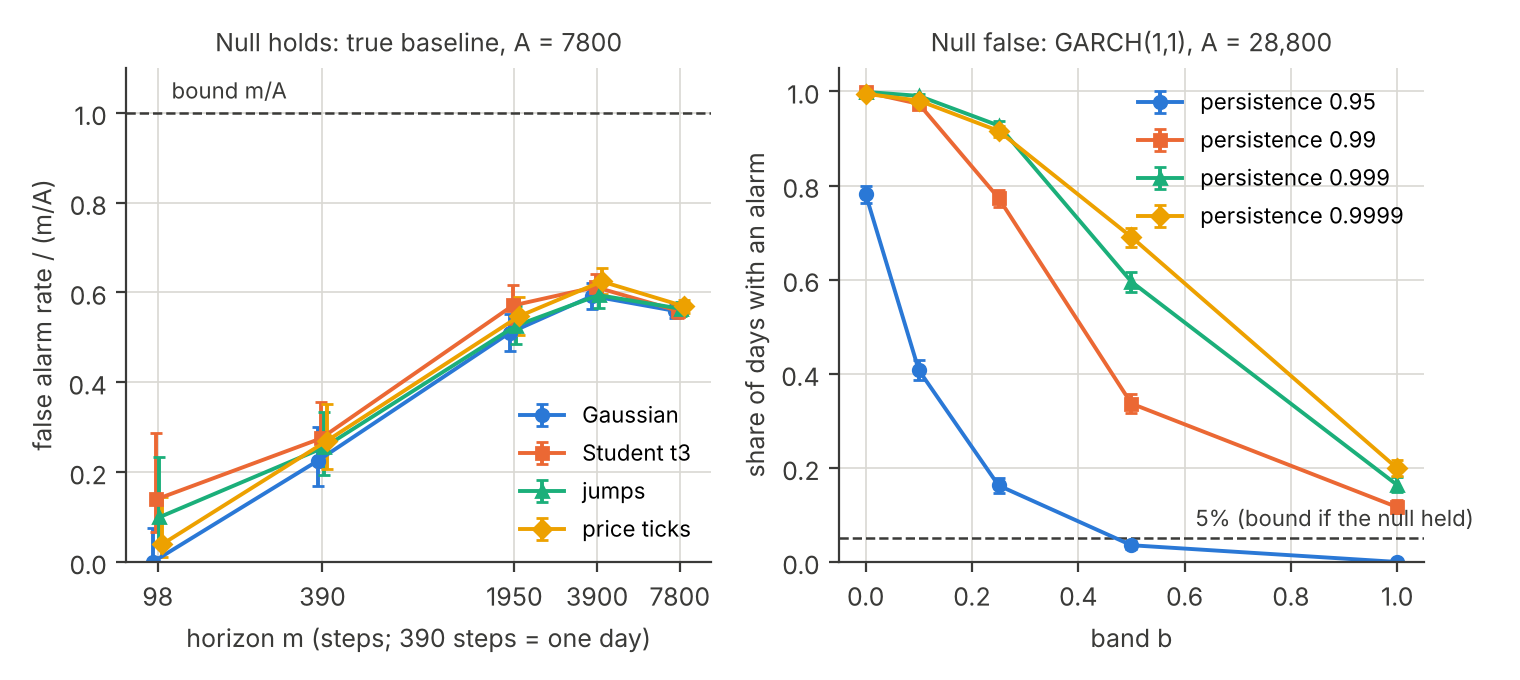
\includegraphics{figures/validity.png}
\caption{Figure 1. Simulated data. Left: false alarm rate within \(m\)
steps divided by the bound \(m/A\), for four return laws with the true
baseline, \(A = 7800\), with 95\% intervals. Right: share of 1440-step
days with an alarm under GARCH(1,1) clustering, where the null is false,
as a function of the band \(b\), \(A = 28{,}800\), with 95\% intervals;
the dashed line is the 5\% that Theorem 4 would give if the null held.}
\end{figure}

With the true baseline, to which the theorems apply, the bound held for
every law, with almost the same rates for all four (Figure 1, left;
Table S4): 1.1\% to 1.4\% at one day against 5\%, and 55.9\% to 56.9\%
at \(m = A\). The bound is conservative by a factor of about 4 at one
day and 2 at \(m = A\), mostly because of expected wealth stranded on
paths that never alarm, but for a single bet of 0.5 a law found by
dynamic programming over the whole nonparametric null reaches 95\% of it
(Supplement S5).

\textbf{An adversarial search.} The worst null stream found, which
watches the detector's own state, alarmed within one day on 2.62\% of
paths (95\% interval 2.50\% to 2.75\%) against the bound of 5\%, and
within five days on 18.1\% against 25\%; outside the class each failure
matched the broken condition (companion note).

\hypertarget{delay-against-parametric-and-robust-competitors}{%
\subsection{6.2 Delay against parametric and robust
competitors}\label{delay-against-parametric-and-robust-competitors}}

With the designs of Table 2 and a change 500 steps into monitoring
(Table S5), the Gaussian likelihood-ratio e-detector detected increases
of the standard deviation by 25\%, 50\% and 100\% in a median of 78, 26
and 10 steps on clean Gaussian data, against 87, 35 and 17 for the
robust detector, an extra delay of 10\% to 70\%, close to Table 1, but
under jumps or fat tails the parametric detectors alarmed before the
change on 74\% to 99\% of paths. Truncation matters under jumps (Table
S5). For decreases the Gaussian detector was faster, at 3\% to 9\% false
alarms before the change, but this rests on normality: real one-minute
returns contain many exact zeros (5.7\% of Bitstamp BTC/USD minutes),
which a Gaussian likelihood reads as low volatility.

\textbf{BOCPD and a two-window scan.} Bayesian online change-point
detection (BOCPD; Adams and MacKay 2007) with a Gaussian model, on raw
or clipped returns, and a two-window variance-ratio scan inspired by
Bibinger, Jirak and Vetter (2017) but of our own construction (footnote
1; Supplement S5) were matched to the e-detector's first-day false alarm
rate on clean Gaussian paths. BOCPD then alarmed within the first day on
73.2\% of paths with jumps and 53.2\% with Student \(t_5\) returns
(e-detector 1.3\% and 1.2\%); clipping fixed jumps (1.6\%) but not fat
tails (7.5\%). On clean Gaussian data BOCPD was faster for large changes
(median 26 against 81 steps for a halving of the standard deviation) but
detected fewer small changes.

\textbf{Competitors calibrated for the data at hand.} We also ran
classical rules on the e-detector's own statistic, and a Student \(t\)
BOCPD and CUSUM monitoring rules with a training sample of the type of
Chu, Stinchcombe and White (1996) and Horváth, Kokoszka and Zhang
(2006), not reproductions (footnote 1); the last two were slower or
missed more small changes (Supplement S5). At its first-day Gaussian
rate (1.3\%), the e-detector's own betting statistic with a simulated
threshold in place of \(2A\) was slightly slower than the e-detector,
and Page's CUSUM on \(X\) was as fast for increases and 15\% to 40\%
faster for decreases, where validity caps the e-detector's bets. But
calibrated thresholds hold only for their calibration law:
Gaussian-calibrated CUSUMs on \(X\) had 5.0\% to 8.2\% first-day false
alarms under Student \(t\) returns, and per-path bootstrap thresholds
were significantly above target in 5 of 24 cells. At a matched rate,
Ville's threshold costs this statistic little delay and adds a guarantee
that needs no calibration.

\hypertarget{the-cost-of-an-estimated-baseline}{%
\subsection{6.3 The cost of an estimated
baseline}\label{the-cost-of-an-estimated-baseline}}

With \(\delta = 0.01\) per side and \(A = 9750\), the
confidence-sequence monitor of Theorem 16 had at most 0.27\% false
alarms in the first day in nine settings without a change (Supplement
S5), and its bound failed on at most 0.08\% of paths against an allowed
1\%; the plug-in was at 4.5\% to 4.9\% on the increase side at 390
calibration steps. The price is delay: 1.8 to 7.6 times the plug-in's
median delay at 390 calibration steps, 1.4 to 3.0 times at 1440 and 1.2
to 1.7 times at 5000, because the confidence bound is wide when
calibration is short (Table S6; Supplement S5).

\hypertarget{when-the-null-is-false-clustering-forecasts-and-price-noise}{%
\subsection{6.4 When the null is false: clustering, forecasts and price
noise}\label{when-the-null-is-false-clustering-forecasts-and-price-noise}}

Under GARCH(1,1) returns with constant unconditional variance and the
true unconditional baseline, the monitor alarmed on 78\% of 1440-step
days at persistence 0.95 and on 100\% at 0.99 or more; a band
\(b = 0.5\) absorbs short-lived clustering, but even \(b = 1\) leaves
12\% to 20\% of days with an alarm when the half-life is an hour or more
(Figure 1, right). Dividing returns by a frozen GARCH(1,1) forecast
(Bollerslev 1986) brought the one-day rate to 3.0\% to 6.2\%, but at
persistence 0.99 a doubling of the long-run variance was detected within
a day on only 34\% to 43\% of paths: with GARCH parameters
\((\omega, \alpha, \beta)\), no break of \(\omega\) lifts the ratio of
the mean squared return to the mean forecast above \((1-\beta)/\alpha\)
(Proposition S13). Price-level noise also breaks the null, but not for a
statistic pre-averaged over non-overlapping blocks of prices, to which
Theorems 3 and 4 apply (Supplement S6).

\hypertarget{extensions}{%
\subsection{6.5 Extensions}\label{extensions}}

\textbf{A null without a baseline.} The \emph{rank detector} bets
\(f(p_t)\) on the smoothed conformal p-value \(p_t\) of Vovk,
Nouretdinov and Gammerman (2003), the share of
\(\lvert r_1\rvert, \dots, \lvert r_t\rvert\) above \(\lvert r_t\rvert\)
with ties split at random, where \(f \ge 0\) and \(\int_0^1 f = 1\). For
exchangeable returns the \(p_t\) are i.i.d. uniform, so Lemma 2 holds in
their filtration and Theorems 3 and 4 hold with no baseline, no \(\tau\)
and no \(\delta\); for i.i.d. returns, and for every infinite
exchangeable sequence, they hold also when the detector restarts at once
after an alarm with an empty reference set (Supplement S1.9). Its null,
exchangeability, neither implies nor is implied by the conditional-mean
null: it needs no baseline, but it excludes all time dependence.

\textbf{Other extensions.} A running truncation level with a band for
all levels, and restarts that learn their band while they monitor, keep
a proof for i.i.d. returns (Supplement S1.9). Restarts remove the blind
period: where volatility moved about once a day, the rank restart
detected 99.6\% of Gaussian changes within a day, against 56\% to 66\%
for monitors that recalibrate. The companion note also treats many
assets, with e-BH (Wang and Ramdas 2022), and several sampling
frequencies.

\hypertarget{application}{%
\section{7 Application}\label{application}}

\hypertarget{data-design-and-what-real-data-can-test}{%
\subsection{7.1 Data, design and what real data can
test}\label{data-design-and-what-real-data-can-test}}

\textbf{Data.} Binance spot one-minute bars for BTC, ETH, XRP, SOL and
DOGE against USDT, with no missing minutes: 1 July to 31 December 2025
(264,959 returns per coin) and, out of sample, 21 January 2024 to 30
June 2025 (527 days), deseasonalised as in Section 2. The monitor uses
\(c = 3\) and the band \(b = 0.25\), each side alarming at \(2A\), and
recalibrates on one day of data after every alarm, with \(A = 28{,}800\)
for the plug-in baseline and \(\delta = 0.01\) and \(A = 36{,}000\) for
the confidence-sequence baseline (5\% for the first 1440-minute day).
The band tolerates slow drift of the conditional variance: under slow
log-normal stochastic volatility it cut the first-day alarm rates from
24.7\% and 26.7\% to 8.3\% (still above 5\%) and 5.0\%, and raised the
median delay to a doubling or a halving of volatility from 19 and 74
steps to 28 and 111 (Supplement S6). The settings were fixed after one
run on Bitstamp BTC/USD for July to December 2025, so only January to
June 2025 is fully held out.

\textbf{What the real data test.} Four pre-registered analyses use
proved monitors, each specified in a document committed before any of
its real-data runs (later decisions are called post hoc): the null
streams below, on which the null holds by construction, the
confidence-sequence configuration of Section 7.2, the rerun of the event
test with a daily restart, and the same test on the releases of 2026,
the only one on data not seen before (Section 7.3). All other real-data
analyses use the plug-in baseline, whose level is measured (Sections 4.1
and 6.1), not proved, and show how the monitor behaves as a tool. Of
these, the FOMC and CPI test on BTC (Section 7.3) is primary, fixed
before the first run in analysis code first saved with its results, and
was not confirmed on the releases of 2026; the Nifty 50 and Budget
analyses, the forecast regressions and the comparisons with classical
rules are secondary (described in advance); the rest is exploratory.
Secondary results carry 95\% intervals from a block bootstrap over
calendar days and p-values adjusted by Holm's (1979) method within
families (Supplement S7.4).

\textbf{Null streams built from real returns.} Real data cannot show
where the null holds, but streams built from real returns can make it
hold; they check the bounds and their slack under the real marginal law
of returns, which no simulation from a parametric law does. The primary
endpoint uses 20,000 streams that permute the returns of the calm days
of July to December 2025, pooled over the five coins (days whose robust
volatility is near its median over the previous 20 days; Supplement
S7.6); they keep the real zeros, ticks and heavy tails and remove all
time dependence, so the null holds exactly for the rank detector and,
for the other monitors, up to the small drift of a finite pool. At band
0 the first-day false alarm probability was 2.26\% (95\% interval 2.06\%
to 2.48\%) with the known baseline, 0.01\% (0.00\% to 0.04\%) with the
confidence-sequence baseline and 3.38\% (3.14\% to 3.64\%) for the rank
detector, against 5\%, and no interval of these three lay above its
bound in any of 252 cells. The plug-in gave 5.50\% (5.19\% to 5.82\%),
and 41\% within five days against 25\%. Streams that bootstrap blocks of
calm days, keeping their real order, made every monitor alarm within a
day on 86\% to 100\% of streams: real minute-level data rarely satisfy
the null, so real alarm rates are not false alarm rates.

\hypertarget{five-cryptocurrencies}{%
\subsection{7.2 Five cryptocurrencies}\label{five-cryptocurrencies}}

\textbf{The confidence-sequence baseline (pre-registered).} In the
primary configuration (July to December 2025, band 0.25), one of the
real-data analyses with a proved monitor (Section 7.1), under the
tolerance of Theorem 16, it raised 0.51 to 0.53 alarms per day per coin,
against 0.66 to 0.70 for the plug-in. These data had already been
analysed with the plug-in, so the pre-registration fixed the
configuration, not the novelty of the data. Of its up alarms 78.2\% were
followed by higher volatility, against 79.6\% for the plug-in
(difference \(-1.3\) points, day-block bootstrap interval \(-5.8\) to
3.2), and of its down alarms 96.3\% by lower volatility, against 88.3\%
(\(+8.0\), 2.7 to 13.7); out of sample, 80.8\% and 90.9\% against 77.9\%
and 84.5\%. Its alarms came later, it monitored more of the time, and in
5 of 7031 segments, all on BTC, it could not raise an increase alarm,
for up to 136 days (post hoc; Supplement S7.6).

\textbf{The plug-in baseline (applied).} With the plug-in baseline the
monitor raised 0.66 to 0.71 alarms per day for every coin in both
periods. Of its increase alarms, 75\% to 84\% were followed by a day
whose robust volatility over the next 1440 minutes was above the
calibration baseline, and of its decrease alarms 83\% to 93\% by a day
below it, against about 50\% at random times with the same delay (pooled
differences 27 and 38 points in July to December 2025, 95\% intervals 22
to 33 and 34 to 44); out of sample the shares fell by 1 to 4 points.

\textbf{Forecasts.} The outcome above partly measures the persistence of
volatility, so at each alarm we also forecast the robust volatility of
the next 1440 minutes (EWMA with a half-life of one day, or HAR; Corsi
2009). In July to December 2025 the next day was on the flagged side of
the EWMA forecast after 78.5\% of the plug-in monitor's up alarms and
80.5\% of its down alarms, against 48.7\% to 51.3\% at random times
(Holm \(p \le 0.0016\)); ratio rules on the last 60 or 240 minutes,
tuned with hindsight to the same alarm counts, reached 73.9\% to 82.3\%,
and only 1 of 48 comparisons with them held after Holm (Table S8;
Supplement S7.3). In hourly regressions the alarms added little to a HAR
forecast that includes the last hour's realised variance (Supplement
S7.4): such a forecast mostly knows that volatility has just moved.

\textbf{Competitors at matched alarm counts.} Against BOCPD and the
two-window scan of Section 6.2, the e-detector's alarms were confirmed
more often in 15 of 16 comparisons with windows fixed before the first
run (Holm-adjusted \(p \le 0.021\)), but not significantly more often
than the decrease alarms of competitors with day-long windows, added
later. Classical rules on the same statistic, matched in the same way,
did as well: the calibrated betting rule and both CUSUMs on \(X\) were
never significantly less precise in 24 comparisons (unadjusted p-values;
Supplement S7.3). So the advantage over BOCPD and the scan may come from
the clipped statistic and the restart design, and the e-detector is not
shown to be more precise than a well-calibrated classical rule.

\hypertarget{scheduled-announcements}{%
\subsection{7.3 Scheduled announcements}\label{scheduled-announcements}}

\textbf{FOMC and CPI: the pre-specified primary test.} For BTC, ETH and
SOL in 2024 and 2025, with 16 FOMC statements, 22 CPI releases and
control windows at the same weekday and clock time, the primary family
(BTC, the streaming monitor, Holm over FOMC and CPI) found an increase
alarm within six hours after 9 of 16 FOMC statements against 14\% of
matched controls (Holm \(p = 0.00025\)); the CPI test was not
significant on BTC (\(p = 0.11\)) but was on ETH and SOL, as secondary
replications. This test used the plug-in baseline, which has no
finite-sample guarantee. Its contrast was not confirmed on the releases
of 2026 (below).

\textbf{The rerun with a proved monitor (pre-registered).} Before any of
its real-data runs, but with the result above known, we pre-registered
the same test on the same releases with the confidence-sequence baseline
restarted at every UTC midnight, whose false alarm probability is at
most \(\delta + m/A = 5\%\) on each day of a segment, marginally, while
the tolerance holds during that day (Corollary S14). The primary test
passed: an up alarm came within six hours of 8 of 16 FOMC statements on
BTC, against 10.9\% of matched controls (Holm \(p = 0.00033\)); CPI on
BTC, a secondary hypothesis, passed but is fragile (Supplement S7.2).
Yet this monitor raised an alarm on 48.1\% to 53.5\% of the UTC days on
which it monitored at least one minute, against the 5\% per day that it
allows under the tolerance: real one-minute returns often break the
tolerance, so the rerun shows a monitor that carries the guarantee
flagging the releases of 2024 and 2025, not the guarantee at work.

\textbf{The test on fresh releases (pre-registered).} Because the rerun
was designed on data already seen, we pre-registered one more test
before loading any return of 2026: the primary monitor of the rerun on
BTC, with one stratified test over the FOMC statements and CPI releases
of January to 24 October 2026 together (6 and 10), chosen for its power
(0.82 at the rates of the rerun, 0.78 for the 16 releases in the data).
It failed: an up alarm came within six hours of 2 of the 16 releases,
against 5.9\% of matched controls (\(p = 0.25\); 95\% interval for the
release rate 3.5\% to 36.0\%), and of 1 of the 6 FOMC statements,
against 10.3\%. No secondary family of this monitor passed after Holm,
and no monitor showed a CPI contrast on any coin. On BTC the monitor was
recalibrating or unable to raise an increase alarm at 5 of the 16
releases, in one segment for 47 days. The rank detector, which is never
blind, flagged 4 of the 6 FOMC statements on each coin (Holm
\(p = 0.016\), 0.033 and 0.055), a secondary result. The FOMC contrast
of 2024 and 2025 is therefore exploratory: the only confirmatory test on
releases not seen before did not confirm it, and with power 0.78 this
says that the contrast was smaller in 2026 or absent, not that there is
none (Supplement S7.2).

\hypertarget{other-data-and-what-the-real-data-say-about-the-method}{%
\subsection{7.4 Other data, and what the real data say about the
method}\label{other-data-and-what-the-real-data-say-about-the-method}}

On the Nifty 50 index (2,361 sessions from April 2017 to October 2026;
secondary, with a configuration pre-registered on 2017 to 2021), 78\% of
the held-out increase alarms and 76\% of the decrease alarms were
followed by a session on the flagged side of the baseline, against 47\%
and 53\% at random times (Holm \(p = 0.0008\)). In a secondary event
analysis, Union Budget sessions were followed by alarms far more often
than ordinary sessions (9 of 11 against 25\%, Holm \(p = 0.0006\) over
five event types); Reserve Bank of India policy days showed no
significant excess (Supplement S7.1).

Two lessons qualify the simulations. With the plug-in the coins raised
2.0 to 2.35 alarms per monitored day (July to December 2025, band 0.25),
far above the budget of 0.05 false alarms per monitored day of Corollary
6, because within real calm days the conditional variance moves (Section
7.1). And a monitor that recalibrates for a day after every alarm is
blind most of the time when alarms come every 1.4 days (about 70\% of
the time in the event study); at the four landmark shocks of Supplement
S7.5, fixed in advance, it was recalibrating at all fifteen crypto
cases, which restarts without a blind period address (Section 6.5).

\hypertarget{discussion}{%
\section{8 Discussion}\label{discussion}}

\textbf{What is new and what is not.} The probabilistic tools (Ville's
inequality, test supermartingales, Shiryaev-Roberts e-detectors,
empirical Bernstein confidence sequences, conformal p-values, the
Bahadur-Savage phenomenon, Lorden's and Lai's lower bounds) are known,
and Theorems 3, 4 and 25 and Proposition 10 are known results or direct
instances of them. To our knowledge, and subject to the caveat in
footnote 1, what we add is their combination for jump-robust online
volatility monitoring, the reading over many days and the daily restart,
the drift bound, the plug-in regime, the bounded statistic with a speed
limit for every deterministic valid rule, a confidence-sequence baseline
with a null that does not depend on the algorithm, the decomposition of
the delay cost, and null streams built from real returns. On real data
the hypotheses of the proofs fail on many days, and the only
confirmatory test on releases not seen before failed (Section 7.3), so
the evidence for the guarantees comes from null streams built from real
returns, and the real-data analyses describe how the monitor behaves as
a tool.

\textbf{Limitations.}

\begin{itemize}
\tightlist
\item
  \emph{The null is a statement about conditional means.} Clustering,
  price-level noise, estimated baselines, errors in the intraday profile
  (which no experiment isolates), a change of tail shape at constant
  volatility and a leverage effect all move it without a structural
  change, and on real calm days it fails within a day. Theorem 9 bounds
  a small drift; the remedies (a band, forecast-relative monitoring,
  non-overlapping blocks, the confidence-sequence baseline) cost speed.
\item
  \emph{Per-period guarantees.} Over many days the plain detector's
  guarantee is an expected count; a bound for every day needs the
  restart of Theorem 8, proved for a known baseline and, marginally, for
  the confidence-sequence baseline (Corollary S14), at a cost in delay.
\item
  \emph{Estimated baselines.} The plug-in keeps its level only
  asymptotically, for horizons \(m = o(\sqrt n)\); the
  confidence-sequence baseline needs long calibration to be fast, can be
  blind to increases after an unusually quiet start of its window (on
  BTC in 2026, for 47 days, at two releases), and was run only with a
  quarter of the window fixing \(\tau\).
\item
  \emph{Speed and precision.} Classical rules on the same statistic,
  calibrated for the law at hand, were as fast for increases, faster for
  decreases and as precise on real data; BOCPD found large decreases two
  to three times faster on clean Gaussian data; against a forecast that
  sees the last hour the alarms added little.
\item
  \emph{Delay theory.} It assumes i.i.d. post-change data and a fixed
  baseline; the delay floor covers a change at the first step and is a
  Monte Carlo estimate; the constant of the second-order expansion is
  heuristic; Theorem 25 is asymptotic.
\item
  \emph{Data and benchmarks.} One-minute bars from public mirrors, no
  tick data and no ground truth; apart from the null streams, one
  confidence-sequence configuration and the two pre-registered event
  tests, the real-data analyses use the plug-in baseline, whose level is
  measured, not proved; the only confirmatory test on data not seen
  before, on the FOMC and CPI releases of 2026, failed (Section 7.3);
  the training-sample rules and the robust BOCPD are of the type of the
  published procedures, not reproductions (footnote 1).
\end{itemize}

\textbf{Open problems.} (1) A certified threshold for mixtures sharper
than \(m/A\): the worst stream found reaches about half of the bound at
one day, but the best proved bound is barely below \(m/A\) (companion
note, Section 4). (2) A running truncation level and a restart without a
blind period that are as fast as the plug-in. (3) A narrower baseline,
for example from a betting confidence sequence. (4) Theory under
clustering: a bound for the mean of the ratio
\(\mathbb{E}[r_t^2/\hat\sigma_t^2]\) that the monitor sees, and a
principled band. (5) Monitoring the truncated variance and the truncated
quarticity under one false alarm budget.

\hypertarget{reproducibility}{%
\section{Reproducibility}\label{reproducibility}}

The code, data manifests and result files are in the accompanying
repository, and all simulations use fixed seeds. Supplement S8 gives the
settings and Supplement S9 the script and result file behind every table
and figure. The real data are one-minute bars from public mirrors of
exchange files (Binance; Bitstamp for one check) and a public archive of
Nifty 50 bars, with event dates checked against published schedules. A
script traces every number of the paper to a committed source.

\hypertarget{references}{%
\section{References}\label{references}}

Issue numbers and DOIs are given where we could confirm them.

Adams, R. P. and MacKay, D. J. C. (2007). Bayesian online changepoint
detection. arXiv:0710.3742.

Andersen, T. G. and Bollerslev, T. (1997). Intraday periodicity and
volatility persistence in financial markets. \emph{Journal of Empirical
Finance} 4(2-3), 115-158. doi:10.1016/S0927-5398(97)00004-2

Andersen, T. G., Dobrev, D. and Schaumburg, E. (2012). Jump-robust
volatility estimation using nearest neighbor truncation. \emph{Journal
of Econometrics} 169(1), 75-93. doi:10.1016/j.jeconom.2012.01.011

Andersen, T. G., Todorov, V. and Zhou, B. (2025). Real-time detection of
local no-arbitrage violations. \emph{Quantitative Economics} 16(2),
459-495. doi:10.3982/QE2585

Bahadur, R. R. and Savage, L. J. (1956). The nonexistence of certain
statistical procedures in nonparametric problems. \emph{Annals of
Mathematical Statistics} 27(4), 1115-1122. doi:10.1214/aoms/1177728077

Bapat, S. R. (2026). A jump and noise robust kernel based estimator of
quarticity for high frequency data. \emph{International Review of
Economics and Finance} 109, 105482. doi:10.1016/j.iref.2026.105482

Barndorff-Nielsen, O. E. and Shephard, N. (2004). Power and bipower
variation with stochastic volatility and jumps. \emph{Journal of
Financial Econometrics} 2(1), 1-37. doi:10.1093/jjfinec/nbh001

Berkes, I., Gombay, E., Horváth, L. and Kokoszka, P. (2004). Sequential
change-point detection in GARCH(p,q) models. \emph{Econometric Theory}
20(6), 1140-1167.

Bibinger, M., Jirak, M. and Vetter, M. (2017). Nonparametric
change-point analysis of volatility. \emph{Annals of Statistics} 45(4),
1542-1578. doi:10.1214/16-AOS1499

Bollerslev, T. (1986). Generalized autoregressive conditional
heteroskedasticity. \emph{Journal of Econometrics} 31(3), 307-327.
doi:10.1016/0304-4076(86)90063-1

Boudt, K., Croux, C. and Laurent, S. (2011). Robust estimation of
intraweek periodicity in volatility and jump detection. \emph{Journal of
Empirical Finance} 18(2), 353-367. doi:10.1016/j.jempfin.2010.11.005

Choe, Y. J. and Ramdas, A. (2024). Combining evidence across
filtrations. arXiv:2402.09698.

Chu, C.-S. J., Stinchcombe, M. and White, H. (1996). Monitoring
structural change. \emph{Econometrica} 64(5), 1045-1065.

Clerico, E. (2025). On the optimality of coin-betting for mean
estimation. \emph{International Journal of Approximate Reasoning} 187,
109550. doi:10.1016/j.ijar.2025.109550

Corsi, F. (2009). A simple approximate long-memory model of realized
volatility. \emph{Journal of Financial Econometrics} 7(2), 174-196.
doi:10.1093/jjfinec/nbp001

Dandapanthula, S. and Ramdas, A. (2025). Multiple testing in
multi-stream sequential change detection. arXiv:2501.04130.

Dette, H. and Gösmann, J. (2020). A likelihood ratio approach to
sequential change point detection for a general class of parameters.
\emph{Journal of the American Statistical Association} 115(531),
1361-1377. doi:10.1080/01621459.2019.1630562

Diebold, F. X. (1986). Modeling the persistence of conditional
variances: a comment. \emph{Econometric Reviews} 5(1), 51-56.

Diebold, F. X. and Mariano, R. S. (1995). Comparing predictive accuracy.
\emph{Journal of Business and Economic Statistics} 13(3), 253-263.

Driscoll, J. C. and Kraay, A. C. (1998). Consistent covariance matrix
estimation with spatially dependent panel data. \emph{Review of
Economics and Statistics} 80(4), 549-560. doi:10.1162/003465398557825

Dufresne, D. (1990). The distribution of a perpetuity, with applications
to risk theory and pension funding. \emph{Scandinavian Actuarial
Journal} 1990(1), 39-79.

Dvoretzky, A., Kiefer, J. and Wolfowitz, J. (1956). Asymptotic minimax
character of the sample distribution function and of the classical
multinomial estimator. \emph{Annals of Mathematical Statistics} 27(3),
642-669. doi:10.1214/aoms/1177728174

Fan, X., Grama, I. and Liu, Q. (2015). Exponential inequalities for
martingales with applications. \emph{Electronic Journal of Probability}
20, paper 1, 1-22. doi:10.1214/EJP.v20-3496

Fearnhead, P. and Rigaill, G. (2019). Changepoint detection in the
presence of outliers. \emph{Journal of the American Statistical
Association} 114(525), 169-183. doi:10.1080/01621459.2017.1385466

Grünwald, P., de Heide, R. and Koolen, W. (2024). Safe testing.
\emph{Journal of the Royal Statistical Society Series B} 86(5),
1091-1128. doi:10.1093/jrsssb/qkae011

Holm, S. (1979). A simple sequentially rejective multiple test
procedure. \emph{Scandinavian Journal of Statistics} 6(2), 65-70.

Honda, J. and Takemura, A. (2010). An asymptotically optimal bandit
algorithm for bounded support models. \emph{Proceedings of the 23rd
Conference on Learning Theory (COLT 2010)}, 67-79.

Horváth, L., Hušková, M., Kokoszka, P. and Steinebach, J. (2004).
Monitoring changes in linear models. \emph{Journal of Statistical
Planning and Inference} 126, 225-251.

Horváth, L., Kokoszka, P. and Zhang, A. (2006). Monitoring constancy of
variance in conditionally heteroskedastic time series. \emph{Econometric
Theory} 22(3), 373-402.

Horváth, L., Trapani, L. and Wang, S. (2025). Sequential monitoring for
changes in GARCH(1,1) models without assuming stationarity.
\emph{Journal of Time Series Analysis} 46(5), 981-996.
doi:10.1111/jtsa.12824

Howard, S. R., Ramdas, A., McAuliffe, J. and Sekhon, J. (2021).
Time-uniform, nonparametric, nonasymptotic confidence sequences.
\emph{Annals of Statistics} 49(2), 1055-1080. doi:10.1214/20-AOS1991

Huber, P. J. (1965). A robust version of the probability ratio test.
\emph{Annals of Mathematical Statistics} 36(6), 1753-1758.
doi:10.1214/aoms/1177699803

Inclán, C. and Tiao, G. C. (1994). Use of cumulative sums of squares for
retrospective detection of changes of variance. \emph{Journal of the
American Statistical Association} 89(427), 913-923.
doi:10.1080/01621459.1994.10476824

Knoblauch, J., Jewson, J. and Damoulas, T. (2018). Doubly robust
Bayesian inference for non-stationary streaming data with β-divergences.
\emph{Advances in Neural Information Processing Systems} 31.

Lai, T. L. (1998). Information bounds and quick detection of parameter
changes in stochastic systems. \emph{IEEE Transactions on Information
Theory} 44(7), 2917-2929. doi:10.1109/18.737522

Lamoureux, C. G. and Lastrapes, W. D. (1990). Persistence in variance,
structural change, and the GARCH model. \emph{Journal of Business and
Economic Statistics} 8(2), 225-234.

Larsson, M., Ramdas, A. and Ruf, J. (2024). The numeraire e-variable and
reverse information projection. arXiv:2402.18810.

Lorden, G. (1970). On excess over the boundary. \emph{Annals of
Mathematical Statistics} 41(2), 520-527. doi:10.1214/aoms/1177697092

Lorden, G. (1971). Procedures for reacting to a change in distribution.
\emph{Annals of Mathematical Statistics} 42(6), 1897-1908.
doi:10.1214/aoms/1177693055

Mancini, C. (2009). Non-parametric threshold estimation for models with
stochastic diffusion coefficient and jumps. \emph{Scandinavian Journal
of Statistics} 36, 270-296.

Massart, P. (1990). The tight constant in the Dvoretzky-Kiefer-Wolfowitz
inequality. \emph{Annals of Probability} 18(3), 1269-1283.
doi:10.1214/aop/1176990746

Mei, Y. (2008). Is average run length to false alarm always an
informative criterion? \emph{Sequential Analysis} 27(4).

Mikosch, T. and Starica, C. (2004). Nonstationarities in financial time
series, the long-range dependence, and the IGARCH effects. \emph{Review
of Economics and Statistics} 86(1), 378-390.
doi:10.1162/003465304323023886

Mineiro, P. (2022). A lower confidence sequence for the changing mean of
non-negative right heavy-tailed observations with bounded mean.
arXiv:2210.11133.

Page, E. S. (1954). Continuous inspection schemes. \emph{Biometrika}
41(1-2), 100-115. doi:10.1093/biomet/41.1-2.100

Patton, A. J. (2011). Volatility forecast comparison using imperfect
volatility proxies. \emph{Journal of Econometrics} 160(1), 246-256.
doi:10.1016/j.jeconom.2010.03.034

Pollak, M. (1985). Optimal detection of a change in distribution.
\emph{Annals of Statistics} 13(1), 206-227. doi:10.1214/aos/1176346587

Pollak, M. (1987). Average run lengths of an optimal method of detecting
a change in distribution. \emph{Annals of Statistics} 15(2), 749-779.
doi:10.1214/aos/1176350373

Ram, A. and Ramdas, A. (2026). Asymptotically optimal sequential change
detection for bounded means. arXiv:2602.05272.

Ramdas, A., Grünwald, P., Vovk, V. and Shafer, G. (2023). Game-theoretic
statistics and safe anytime-valid inference. \emph{Statistical Science}
38(4), 576-601. doi:10.1214/23-STS894

Roberts, S. W. (1966). A comparison of some control chart procedures.
\emph{Technometrics} 8(3), 411-430.

Shafer, G. (2021). Testing by betting: a strategy for statistical and
scientific communication. \emph{Journal of the Royal Statistical Society
Series A} 184(2), 407-431. doi:10.1111/rssa.12647

Shekhar, S. and Ramdas, A. (2024). Reducing sequential change detection
to sequential estimation. \emph{Proceedings of the International
Conference on Machine Learning (ICML 2024)}, PMLR 235, 44628-44642.

Shin, J., Ramdas, A. and Rinaldo, A. (2024). E-detectors: a
nonparametric framework for sequential change detection. \emph{New
England Journal of Statistics in Data Science} 2(2), 229-260.
doi:10.51387/23-NEJSDS51

Shiryaev, A. N. (1963). On optimum methods in quickest detection
problems. \emph{Theory of Probability and Its Applications} 8(1), 22-46.
doi:10.1137/1108002

Tartakovsky, A., Nikiforov, I. and Basseville, M. (2014).
\emph{Sequential Analysis: Hypothesis Testing and Changepoint
Detection}. Chapman and Hall/CRC.

Unnikrishnan, J., Veeravalli, V. V. and Meyn, S. (2009). Minimax robust
quickest change detection. arXiv:0911.2551.

Ville, J. (1939). \emph{Étude critique de la notion de collectif}.
Thèse, Paris.

Vovk, V., Nouretdinov, I. and Gammerman, A. (2003). Testing
exchangeability on-line. \emph{Proceedings of the 20th International
Conference on Machine Learning (ICML 2003)}, 768-775.

Vovk, V., Petej, I., Nouretdinov, I., Ahlberg, E., Carlsson, L. and
Gammerman, A. (2021). Retrain or not retrain: conformal test martingales
for change-point detection. \emph{Proceedings of Machine Learning
Research} 152, 191-210.

Wang, H. and Ramdas, A. (2023). Huber-robust confidence sequences.
\emph{Proceedings of the International Conference on Artificial
Intelligence and Statistics (AISTATS 2023)}, PMLR 206, 9662-9679.

Wang, Q., Wang, R. and Ziegel, J. (2026). E-backtesting.
\emph{Management Science} 72(6), 4952-4973. doi:10.1287/mnsc.2023.01659

Wang, R. and Ramdas, A. (2022). False discovery rate control with
e-values. \emph{Journal of the Royal Statistical Society Series B}
84(3), 822-852. doi:10.1111/rssb.12489

Waudby-Smith, I. and Ramdas, A. (2024). Estimating means of bounded
random variables by betting. \emph{Journal of the Royal Statistical
Society Series B} 86(1), 1-27. doi:10.1093/jrsssb/qkad009

Woodroofe, M. (1982). \emph{Nonlinear Renewal Theory in Sequential
Analysis}. CBMS-NSF Regional Conference Series in Applied Mathematics
39. SIAM, Philadelphia.

Zeileis, A., Leisch, F., Hornik, K. and Kleiber, C. (2002). strucchange:
An R package for testing for structural change in linear regression
models. \emph{Journal of Statistical Software} 7(2), 1-38.
doi:10.18637/jss.v007.i02

\hypertarget{supplementary-material}{%
\section{Supplementary material}\label{supplementary-material}}

The supplement holds the proofs of the results of the main text, the
details of several results that the main text summarises, the settings
of every experiment and a map from each table and figure to its script
and result file. Section, table and figure numbers refer to the main
text unless they start with S. Supplement S1.9 proves the results behind
the rank detector, the running truncation level and the restarts of
Section 6.5. A companion note, \texttt{paper/extensions.md}, reports the
experiments on these extensions, treats the others summarised in Section
6.5 and the adversarial search of Section 6.1.

\hypertarget{s1.-proofs-and-details-for-sections-2-and-3}{%
\subsection{S1. Proofs and details for Sections 2 and
3}\label{s1.-proofs-and-details-for-sections-2-and-3}}

\hypertarget{s1.1-corollary-6-proof-and-numbers}{%
\subsubsection{S1.1 Corollary 6: proof and
numbers}\label{s1.1-corollary-6-proof-and-numbers}}

Let \(W_t\) be the sum of \(\bar M\) at all past alarms, plus the
current \(\bar M\), minus the number of monitored steps so far. By Lemma
2 applied in each segment, \(W\) is a supermartingale with \(W_0 = 0\):
at an alarm the statistic moves into the sum unchanged, and calibration
steps leave \(W\) unchanged. Each alarm adds at least \(A\) to the sum.
Optional stopping at the bounded time \(\vartheta \wedge n\), with
\(\vartheta\) the time of the \(m\)-th monitored step, and monotone
convergence as \(n \to \infty\) give \(A\,\mathbb{E}[N_m] - m \le 0\).
\(\square\)

\emph{Numbers.} With the true baseline and \(A = 300\) the restarted
monitor raised 26.5 alarms per 10,000 monitored steps against the bound
of 33.3; with the confidence-sequence baseline and \(A = 36{,}000\) it
raised 0.000 (Gaussian) and 0.001 (Student \(t_3\)) false alarms per
1440-step day in 30-day streams, against a bound of 0.041. At operating
levels with a known baseline, the monitor restarted after every alarm
raised 0.037 to 0.048 false alarms per day over 20 days at \(A = 7800\)
and \(28{,}800\) (Supplement S1.7), and 0.040 per monitored day on null
streams built from real returns (Supplement S7.6), against the 0.05 of
Corollary 6.

\hypertarget{s1.2-theorem-9-proof-design-numbers-and-sharpness}{%
\subsubsection{S1.2 Theorem 9: proof, design numbers and
sharpness}\label{s1.2-theorem-9-proof-design-numbers-and-sharpness}}

For one bet write \(R_t = f_t(R_{t-1} + 1)\) with \(R_0 = 0\), so that
\(M_t = \sum_k w_k R_t^{(k)}\) on each side.

\textbf{Lemma S1 (expected wealth under a drift).} Let \(f_t \ge 0\) be
adapted and bounded, and let \(h_1, h_2, \dots\) be numbers at least 1
with \(\mathbb{E}[f_t \mid \mathcal{F}_{t-1}] \le h_t\) for every \(t\).
Then for every stopping time \(T\) (possibly infinite) and every
\(t \ge 0\),
\(\mathbb{E}[R_{T \wedge t}] \le s_t := \sum_{j=1}^{t}\prod_{i=j}^{t} h_i\).
With a constant \(h_i = 1 + x\), \(s_t = t\,\Upsilon_t(x)\).

\emph{Proof.} Put \(a_t = \mathbb{E}[R_{T\wedge t}]\), which is finite
because the factors are bounded. Split
\(R_{T\wedge t} = R_T 1\lbrace T \le t-1\rbrace + R_t 1\lbrace T > t-1\rbrace\).
The event \(\lbrace T > t-1\rbrace\) is known at time \(t-1\), so
\(\mathbb{E}[R_t 1\lbrace T > t-1\rbrace] = \mathbb{E}[1\lbrace T > t-1\rbrace\,\mathbb{E}[f_t \mid \mathcal{F}_{t-1}](R_{t-1} + 1)] \le h_t\,\mathbb{E}[1\lbrace T > t-1\rbrace(R_{t-1} + 1)]\).
Because \(h_t \ge 1\) and \(R \ge 0\), also
\(\mathbb{E}[R_T 1\lbrace T \le t-1\rbrace] \le h_t\,\mathbb{E}[R_T 1\lbrace T \le t-1\rbrace]\).
Adding gives
\(a_t \le h_t(a_{t-1} + \mathbb{P}(T > t-1)) \le h_t(a_{t-1} + 1)\).
Since \(a_0 = 0 = s_0\) and \(s_t = h_t(s_{t-1} + 1)\), induction gives
\(a_t \le s_t\). \(\square\)

\emph{Proof of Theorem 9.} On the increase side
\(\mathbb{E}[f_t^{(k)} \mid \mathcal{F}_{t-1}] = 1 + \lambda_k^{\uparrow}(\mu_t/m^{\uparrow} - 1) \le 1 + \lambda_k^{\uparrow}\xi^{\uparrow}\),
and on the decrease side
\(\mathbb{E}[f_t^{(l)} \mid \mathcal{F}_{t-1}] = 1 + \lambda_l^{\downarrow}(1 - \mu_t/m^{\downarrow}) \le 1 + \lambda_l^{\downarrow}\xi^{\downarrow}\).
An alarm of the two-sided rule at \(T_A \le m\) implies
\(\bar M_{T_A \wedge m} \ge A\), and \(\bar M \ge 0\), so
\(A\,\mathbb{P}(T_A \le m) \le \mathbb{E}[\bar M_{T_A \wedge m}]\).
Lemma S1 with \(h_t = 1 + \lambda_k^{\uparrow}\xi^{\uparrow}\) bounds
the expected wealth of increase bet \(k\) at \(T_A \wedge m\) by
\(m\,\Upsilon_m(\lambda_k^{\uparrow}\xi^{\uparrow})\), and likewise on
the decrease side. Averaging with the weights and over the two sides
gives \(\mathbb{E}[\bar M_{T_A \wedge m}] \le m\,\Gamma_m\). When
\(\xi^{\uparrow}\) and \(\xi^{\downarrow}\) are random but known at time
0, apply Lemma S1 conditionally on \(\mathcal{F}_0\). \(\square\)

\emph{Proof of Corollary 14.} Given the window, \(\hat\tau\),
\(\hat m\), the bets and the drifts \(\xi^{\uparrow}(W)\) and
\(\xi^{\downarrow}(W)\) are known at time 0, and the conditional means
stay within these drifts by assumption. Theorem 9 conditionally on
\(\mathcal{F}_0\) gives
\(\mathbb{P}(T_A \le m \mid \mathcal{F}_0) \le \min\lbrace 1, (m/A)\,\Gamma_m(\xi^{\uparrow}(W), \xi^{\downarrow}(W))\rbrace\);
take expectations over the window. \(\square\)

\textbf{Design numbers.} Table S1 gives the inflation factor for the
default detector with \(c = 3\), \(b = 0\) and \(A = 7800\), for a drift
of \(\xi\) on both sides; the bound is \(\min(1, (m/A)\,\Gamma_m)\). At
one day a drift of 0.1\%, 0.5\% and 1\% on both sides gives 5.14\%,
5.80\% and 7.06\% instead of 5\%. To first order
\(\Gamma_m \approx 1 + (m+1)(\bar\lambda^{\uparrow}\xi^{\uparrow} + \bar\lambda^{\downarrow}\xi^{\downarrow})/4\),
with \(\bar\lambda\) the weighted mean bet of each side, while the
largest bet times the drift times \(m\) is small; beyond that it grows
like \((1 + \lambda_{\max}\xi)^m\). The one-day bound reaches 10\% at a
drift of 1.63\% and 25\% at 2.66\% on both sides; with an upward drift
only (a conditional mean between \(m_0\) and \(m_0(1 + \xi)\)) at 1.72\%
and 2.70\%; with a downward drift only at 6.36\% and 10.51\%, because
the decrease bets are smaller; and for a 1440-step day with
\(A = 28{,}800\), at 0.44\% and 0.72\%.

\begin{longtable}[]{@{}
  >{\raggedright\arraybackslash}p{(\columnwidth - 6\tabcolsep) * \real{0.2500}}
  >{\raggedright\arraybackslash}p{(\columnwidth - 6\tabcolsep) * \real{0.2500}}
  >{\raggedright\arraybackslash}p{(\columnwidth - 6\tabcolsep) * \real{0.2500}}
  >{\raggedright\arraybackslash}p{(\columnwidth - 6\tabcolsep) * \real{0.2500}}@{}}
\toprule\noalign{}
\begin{minipage}[b]{\linewidth}\raggedright
drift \(\xi\) on both sides
\end{minipage} & \begin{minipage}[b]{\linewidth}\raggedright
\(\Gamma_m\), one day
\end{minipage} & \begin{minipage}[b]{\linewidth}\raggedright
\(\Gamma_m\), five days
\end{minipage} & \begin{minipage}[b]{\linewidth}\raggedright
first horizon at which the bound reaches 1
\end{minipage} \\
\midrule\noalign{}
\endhead
\bottomrule\noalign{}
\endlastfoot
0.10\% & 1.027 & 1.160 & 4,880 \\
0.50\% & 1.160 & 4.239 & 1,919 \\
1.00\% & 1.412 & 158 & 1,140 \\
2.00\% & 2.638 & \(1.2 \times 10^6\) & 654 \\
3.00\% & 7.452 & \(1.2 \times 10^{10}\) & 468 \\
\end{longtable}

\emph{Table S1. Inflation factor of Theorem 9 for the default detector,
\(c = 3\), \(b = 0\), \(A = 7800\); a day is 390 steps. Closed form, no
simulation.}

\textbf{Proposition S2 (where the bound is attained).} For one side with
one bet \(\lambda\) at level \(A\), the deterministic stream
\(Y_t = 1 + \xi\) (allowed when \(1 + \xi \le B\)) satisfies the
hypothesis of Theorem 9 with equality and alarms at
\(m^\ast = \min\lbrace t : t\,\Upsilon_t(\lambda\xi) \ge A\rbrace\). No
bound of the form \(c\,m\,\Upsilon_m(\lambda\xi)/A\) that is valid for
this stream can have \(c < 1/((1 + \lambda\xi)(1 + 1/A))\) at
\(m = m^\ast\).

\emph{Proof.} Every factor equals \(1 + \lambda\xi\), so
\(R_t = t\,\Upsilon_t(\lambda\xi)\) and the alarm time is \(m^\ast\)
with probability 1. Since
\(R_{m^\ast} = (1 + \lambda\xi)(R_{m^\ast - 1} + 1) < (1 + \lambda\xi)(A + 1)\),
a valid bound \(c R_{m^\ast}/A \ge 1\) needs
\(c > A/((1 + \lambda\xi)(A + 1))\). \(\square\)

For the default two-sided detector the one-day bound reaches 1 at an
upward drift of 3.740\%, and the deterministic stream alarms within the
day from 3.756\%. Below that drift the deterministic stream does not
alarm within the day, and the strongest stream we found, which holds
\(Y_t\) at its mean for a searched number of steps and then plays bold
(Section 6.1), reaches 0.33 to 0.63 of the bound in one day; the worst
case there is open. Noisy streams are far below the bound: the two-point
law \(\lbrace 0, B\rbrace\) gives 2.0\% in one day at a drift of 0.25\%
and 2.4\% at 5\%.

\hypertarget{s1.3-a-drift-that-varies}{%
\subsubsection{S1.3 A drift that
varies}\label{s1.3-a-drift-that-varies}}

Theorem 9 needs a bound on the drift at every step. Under GARCH
clustering the conditional mean comes arbitrarily close to \(\tau^2\)
when \(\sigma_t\) is large, so the only valid constant is
\(\xi^{\uparrow} = B - 1\) and the bound is 1, although the drift
averages out over time. Take \(b = 0\), so both sides normalise by
\(m_0\), and let \(d_t = \mathbb{E}[Y_t \mid \mathcal{F}_{t-1}] - 1\) be
the signed drift.

\textbf{Lemma S3 (a pathwise inequality).} Let \(u_t^{\uparrow}\) and
\(u_t^{\downarrow}\) be predictable with \(u_t^{\uparrow} \ge d_t\),
\(u_t^{\downarrow} \ge -d_t\), \(u_t^{\uparrow} \ge -1\) and
\(u_t^{\downarrow} \ge 1 - B\), and put
\(h_{k,t}^{\uparrow} = 1 + \lambda_k^{\uparrow}u_t^{\uparrow}\) and
\(h_{l,t}^{\downarrow} = 1 + \lambda_l^{\downarrow}u_t^{\downarrow}\).
Build the two-sided average \(\tilde M_t\) of the Shiryaev-Roberts
statistics of the drift-corrected factors
\(f_t^{(k)}/h_{k,t}^{\uparrow}\) and \(f_t^{(l)}/h_{l,t}^{\downarrow}\).
Then (1) \(\tilde M\) satisfies Lemma 2, so
\(\mathbb{P}(\max_{t \le m}\tilde M_t \ge a) \le m/a\) for every
\(a > 0\); and (2) path by path \(\bar M_t \le D_t^\ast \tilde M_t\),
where \(D_t^\ast\) is the largest window product
\(\prod_{i=j}^{t} h_{k,i}^{\uparrow}\) or
\(\prod_{i=j}^{t} h_{l,i}^{\downarrow}\) over all bets and all starts
\(j \le t\).

\emph{Proof.} (1) The corrected factors have conditional mean at most 1,
so Lemma 2 and the proof of Theorem 4 apply. (2) The wealth of a bet
started at \(j\) is the corrected wealth times the window product, which
is at most \(D_t^\ast\); sum over \(j\) and average over bets and sides.
\(\square\)

\textbf{Theorem S4 (threshold form).} For every predictable drift, every
\(m \ge 1\) and every \(K > 0\),
\(\mathbb{P}(T_A \le m) \le K m/A + \mathbb{P}(\max_{t \le m} D_t^\ast > K)\).

\emph{Proof.} On \(\lbrace T_A \le m\rbrace\),
\(A \le \bar M_{T_A} \le D_{T_A}^\ast \tilde M_{T_A}\), so either
\(\max_{t \le m} D_t^\ast > K\) or \(\tilde M_{T_A} \ge A/K\), which has
probability at most \(Km/A\) by Lemma S3. \(\square\)

A calm spell shrinks the window products and the maximum restarts, so a
drift that averages out does not accumulate. No independence is needed:
the drift may respond to the data, as under GARCH.

\textbf{Theorem S5 (a drift that does not respond to the data).} Suppose
there is a \(\sigma\)-field \(\mathcal{D}\) and
\(\mathcal{D}\)-measurable \(u_t^{\uparrow}, u_t^{\downarrow}\) as in
Lemma S3 with
\(\mathbb{E}[Y_t \mid \mathcal{F}_{t-1} \vee \mathcal{D}] \le 1 + u_t^{\uparrow}\)
and \(\ge 1 - u_t^{\downarrow}\) for every \(t\), and put
\(\xi_t^{\uparrow} = (u_t^{\uparrow})^+\) and
\(\xi_t^{\downarrow} = (u_t^{\downarrow})^+\). Then \[
\mathbb{P}(T_A \le m \mid \mathcal{D}) \le \min\Big\lbrace 1,\ \frac{1}{2A}\Big[\sum_k w_k^{\uparrow}\sum_{j=1}^{m}\prod_{i=j}^{m}(1 + \lambda_k^{\uparrow}\xi_i^{\uparrow}) + \sum_l w_l^{\downarrow}\sum_{j=1}^{m}\prod_{i=j}^{m}(1 + \lambda_l^{\downarrow}\xi_i^{\downarrow})\Big],\ \big(\max_{t \le m} D_t^\ast\big)\frac{m}{A}\Big\rbrace,
\] with \(D^\ast\) built from the \(\mathcal{D}\)-measurable bounds.

\emph{Proof.} Work with the filtration
\(\mathcal{F}_t \vee \mathcal{D}\). The first term is Lemma S1
conditionally on \(\mathcal{D}\), with the fixed numbers
\(1 + \lambda\xi_t \ge 1\), followed by the argument of Theorem 9. The
second is Theorem S4 conditionally on \(\mathcal{D}\) with
\(K = \max_{t \le m} D_t^\ast\), which is \(\mathcal{D}\)-measurable, so
the remainder vanishes. \(\square\)

Examples are a deterministic drift (a known error in the intraday
profile), a drift decided by the calibration window (the plug-in), and
stochastic volatility independent of the innovations. The maximum over
\(t\) is needed: with \(Y_t = B\) for 7 steps and then \(0.95\), the
default detector alarms at step 7, so \(\mathbb{P}(T_A \le 390) = 1\),
while the largest window product ending at step 390 is 17.5 and
\(17.5 \times 390/7800 = 0.876\); the maximum over \(t \le 390\) is
80,628. For a \(\pm 10\%\) drift that flips at every step, Theorem S5
gives 15.3\% at one day, where Theorem 9 gives 1 and the measured rate
is 0.73\%.

\textbf{What cannot be said.} (a) When the drift responds to the data,
the formula of Theorem S5 with the realised drift is not a bound: if
\(Y_1 = B\) with probability \(1/B\) and 0 otherwise, the stream then
stays at \(B\) until the alarm (after \(Y_1 = B\)) or at 1 (after
\(Y_1 = 0\)), the formula gives 10.2\% at one day while the alarm
probability is 11.1\%. This is the GARCH mechanism, in which a large
return raises the next conditional variance, so for GARCH only Theorem
S4 is proved. On 64 GARCH(1,1) designs it was below 1 in 22 at one day,
all with a small drift, at 6 to 29 times the measured rate. (b) The mean
drift alone gives no bound: a coin decided before monitoring that, with
probability \(p\), sets \(Y_t = B\) for the 7 steps the detector needs
to alarm has \(\mathbb{P}(T_A \le m) = p\) while its mean drift is
proportional to \(p/m\), so no inequality
\(\mathbb{P}(T_A \le m) \le C(\bar\xi)\,m/A\) with \(C\) depending only
on the mean drift \(\bar\xi\) holds for all \(A\). A bound in the mean
drift exists only with an additive term weighted by \(A\), which exceeds
the whole one-day budget once the mean upward drift exceeds 0.026\%.

\hypertarget{s1.4-proof-of-corollary-11}{%
\subsubsection{S1.4 Proof of Corollary
11}\label{s1.4-proof-of-corollary-11}}

Fix \(t\), a path \((x_1, \dots, x_t)\) and \(\varepsilon \in (0, 1)\).
Build \(P_\varepsilon \in \mathcal{P}^{\downarrow}\) step by step. If
the past agrees with \((x_1, \dots, x_{s-1})\) and \(x_s^2 \ge m_0\),
draw \(r_s = x_s\); if \(x_s^2 < m_0\), draw \(r_s = x_s\) with
probability \(1 - \varepsilon\) and \(r_s = z_s\) otherwise, with
\(z_s^2 = (m_0 - (1-\varepsilon)x_s^2)/\varepsilon\), so that the
conditional mean of \(r_s^2\) is exactly \(m_0\). Off the path, and
after time \(t\), draw \(r_s = \sqrt{m_0}\). Then
\(P_\varepsilon(r_1 = x_1, \dots, r_t = x_t) \ge (1-\varepsilon)^t\)
and, since \(W_t \ge 0\),
\(1 \ge \mathbb{E}_{P_\varepsilon}[W_t] \ge (1-\varepsilon)^t\, W_t(x_1, \dots, x_t)\).
Let \(\varepsilon \to 0\). For the last claim, each started process is
at most 1, so \(M_t \le t\). \(\square\)

\hypertarget{s1.5-proofs-of-lemma-1-theorem-3-proposition-5-and-proposition-10}{%
\subsubsection{S1.5 Proofs of Lemma 1, Theorem 3, Proposition 5 and
Proposition
10}\label{s1.5-proofs-of-lemma-1-theorem-3-proposition-5-and-proposition-10}}

\textbf{Proof of Lemma 1.} For each fixed \(\varepsilon\),
\(s \mapsto \min(s^2\varepsilon^2, \tau^2)\) is nondecreasing, with
derivative \(2s\varepsilon^2\) where \(s\lvert\varepsilon\rvert < \tau\)
and 0 elsewhere. Since \(\sigma_t\) and \(\tau\) are
\(\mathcal{F}_{t-1}\)-measurable and \(\varepsilon_t\) is independent of
\(\mathcal{F}_{t-1}\), \(\mu_t = g_\tau(\sigma_t)\), and monotonicity
and the derivative pass through the expectation. \(\square\)

\textbf{Proof of Theorem 3.} If \(\mathbb{E}[T_A] = \infty\) there is
nothing to show; otherwise \(T_A < \infty\) almost surely. Optional
stopping of \(M_t - t\) (Lemma 2) at the bounded time \(T_A \wedge t\)
gives
\(\mathbb{E}[M_{T_A \wedge t}] \le \mathbb{E}[T_A \wedge t] \le \mathbb{E}[T_A]\).
As \(t \to \infty\), \(M_{T_A \wedge t} \to M_{T_A} \ge A\), and Fatou's
lemma gives \(A \le \mathbb{E}[T_A]\). \(\square\)

\textbf{Proof of Proposition 5.} Both sides satisfy Lemma 2 under the
two-sided null, so their average does, and
\(\max(M^{\uparrow}, M^{\downarrow}) \ge 2A\) implies \(\bar M \ge A\)
because both statistics are nonnegative. \(\square\)

\textbf{Proof of Proposition 10.} For \(y \ge 1\) the point mass
\(\delta_y\) lies in \(\mathcal{N}_\infty\), so \(E(y) \le 1\). For
\(y < 1\) and \(\varepsilon \in (0, 1)\), let
\(z = (1 - (1-\varepsilon)y)/\varepsilon\), so that
\((1-\varepsilon)\delta_y + \varepsilon \delta_z\) has mean exactly 1.
Then \((1-\varepsilon)E(y) + \varepsilon E(z) \le 1\), and since
\(E \ge 0\), \(E(y) \le 1/(1-\varepsilon)\). Let \(\varepsilon \to 0\).
\(\square\)

\hypertarget{s1.6-proof-of-theorem-12-and-corollary-13}{%
\subsubsection{S1.6 Proof of Theorem 12 and Corollary
13}\label{s1.6-proof-of-theorem-12-and-corollary-13}}

\emph{The largest probability of one value.} Let \(y \in [0, B]\). Under
the decrease null, a law on \([0, B]\) with mean at least 1 and
\(p = \mathbb{P}(Y = y)\) satisfies \(1 \le py + (1 - p)B\), so
\(p \le (B-1)/(B-y)\) when \(y < 1\); the law with mass \((B-1)/(B-y)\)
at \(y\) and the rest at \(B\) has mean exactly 1 and attains it, and
for \(y \ge 1\) the point mass at \(y\) is in the null. Under the
increase null, \(1 \ge \mathbb{E}Y \ge py\) gives \(p \le 1/y\) for
\(y > 1\), attained by the law on \(\lbrace 0, y\rbrace\) with mass
\(1/y\) at \(y\). Under the two-sided null the same two-point laws have
mean exactly 1. So \(\pi\) of Section 3.3 is the largest probability of
\(y\) in each null, attained by a law with mean 1, or by a point mass
when \(\pi(y) = 1\). For \(c = 3\) and Gaussian truncation
(\(B = 9.045\)), \(\pi(0) = 0.889\): a null law can put 89\% of its mass
on a zero return.

\emph{Proof of Theorem 12.} Fix a path \(y\) and \(n\). For \(s \le n\)
let \(Q_s\) be the law just described for \(y_s\), and
\(Q_s = \delta_1\) for \(s > n\); let \(P_y\) make \(Y_1, Y_2, \dots\)
independent with laws \(Q_1, Q_2, \dots\). Each conditional mean is that
of \(Q_s\), so \(P_y\) is in the null, and
\(P_y(Y_{1:n} = y_{1:n}) = \prod_{s \le n}\pi(y_s) = 1/\Pi_n(y) > 0\).
(a) The event \(\lbrace T \le n\rbrace\) is a set of values of
\(Y_{1:n}\); if it contains \(y_{1:n}\), then
\(n/A \ge P_y(T \le n) \ge 1/\Pi_n(y)\). (b) If \(T = T(Y, U)\) with
\(U\) uniform and independent of the data, Fubini's theorem gives
\(n/A \ge P_y(T \le n) \ge \mathbb{P}_U(T(y, U) \le n)/\Pi_n(y)\). (c)
For any law \(P\) in the null and
\(E_s = \lbrace Y_{1:s} = y_{1:s}\rbrace\), the conditional law of
\(Y_s\) given \(E_{s-1}\), when \(P(E_{s-1}) > 0\), has its mean on the
null side, so \(P(Y_s = y_s \mid E_{s-1}) \le \pi(y_s)\) and
\(P(E_n) \le 1/\Pi_n(y)\). The rule ``stop at \(n\) if
\(Y_{1:n} = y_{1:n}\), otherwise never'' therefore has
\(\mathbb{P}(T \le k) = 0\) for \(k < n\) and
\(\mathbb{P}(T \le k) \le 1/\Pi_n(y) \le n/A \le k/A\) for \(k \ge n\).

If the null is stated for the returns, the two-point laws can be placed
on \(\lbrace r_s, \tau\rbrace\) (decrease) or \(\lbrace r_s, 0\rbrace\)
(increase) with the same masses, so the floor also holds for rules that
see \(r_t\), and for rules that use other information whose law the null
leaves free. The proof uses independent laws that are not identically
distributed. If validity were required only over i.i.d. null laws, the
floor would be the largest i.i.d. null probability of the path, which is
never larger than \(1/\Pi_n(y)\) and equals it on paths with one
repeated value, such as the collapse. \(\square\)

\emph{Proof of Corollary 13.} (a) The decrease null on \([0, \infty)\)
contains the decrease null on \([0, B']\) for every
\(B' > \max_{s \le n} y_s\), and \((B'-1)/(B'-y) \to 1\) as
\(B' \to \infty\), so \(\Pi_n(y)\) can be made as close to 1 as we like,
and Theorem 12(a) needs \(1 \ge A/n\), that is \(n \ge A\); by Theorem
12(b) a randomised valid rule alarms by step \(n\) with probability at
most \(n/A\) times a factor that can be made as close to 1 as we like.
(b) On the collapse \(\Pi_n = (B/(B-1))^n\). \(\square\)

\emph{Numbers.} With Gaussian truncation the collapse floor for every
deterministic valid rule is 23, 33, 45, 73 and 106 steps at
\(c = 2, 2.5, 3, 4\) and 5 for \(A = 7800\) (25, 36, 50, 82 and 120 at
\(2A\)), against 28.7, 41.8, 57.7, 95.9 and 140.8 for a Shiryaev-Roberts
e-detector with linear bets and 36, 52, 73, 122 and 180 for the default
grid (63.6 and 79 at \(2A\) for \(c = 3\)). On the collapse a single bet
just below \(\lambda_{\max}\) gives \(M_n \le B(F^n - 1)\) with
\(F = B/(B-1)\), so no Shiryaev-Roberts e-detector whose bets are valid
over the whole null can alarm before
\(n = \log(1 + A/B)/\log(B/(B-1))\). A deterministic valid rule needs
only \(\Pi_n = (B/(B-1))^n \ge A/n\) (Theorem 12(a)), while the
e-detector needs \((B/(B-1))^n \ge 1 + A/B\). The two thresholds differ
by the factor \((1 + A/B)\,n/A\), which is about \(n/B\) because \(A/B\)
is large, and this factor accounts for the gap between 45 and 57.7 steps
at \(c = 3\): the e-detector must keep \(\mathbb{E}M_n \le n\) under
every null law at once, while a valid rule may spend its whole budget
\(n/A\) on one path. On a complete explosion, \(y_s = B\) for every
\(s\), the floor for the increase side is 4 steps at \(c = 3\), against
5 for the e-detectors and 7 for the default grid. A rule valid at one
horizon only, with \(\mathbb{P}(T \le 390) \le 0.05\), could alarm on
the collapse after 26 steps at \(c = 3\), so controlling every \(n\) at
once costs 19 steps on this path. For randomised rules, the largest
probability of an alarm by step \(n\) on the collapse is
\(\min(1, n\Pi_n/A)\): 0.13 at \(n = 30\), 0.56 at 40, 0.85 at 43 and
0.98 at 44. Summing \(1 - \min(1, n\Pi_n/A)\) over \(n\) bounds the mean
delay of such a rule on the collapse from below by only 37.8, because
each cap spends the whole budget \(n/A\) at its own \(n\), while a valid
rule must respect every \(n\) at once. Let \(p_k\) be the probability
that the rule stops at step \(k\) on the collapse path, with
\(\sum_k p_k = 1\). Under the i.i.d. law with mass \((B-1)/B\) at 0 and
\(1/B\) at \(B\), which has mean 1 and lies in the decrease and the
two-sided null, the collapse path up to step \(k\) has probability
\(((B-1)/B)^k\), so validity requires
\(\sum_{k \le n} p_k((B-1)/B)^k \le n/A\) for every \(n\); by the
argument of Theorem 12(c) these constraints also suffice for a rule that
stops only on the collapse path. The smallest mean delay
\(\sum_k k\,p_k\) under them, a linear programme, is 43.39 steps.
Corollary 13 does not mean that a practical rule detects collapses after
45 steps from any starting point: a rule that tests disjoint blocks of
45 steps for all-zero returns is valid, but finds a collapse that starts
inside a block only at the end of the next block.

\hypertarget{s1.7-later-days-proposition-7-theorem-8-the-delay-of-the-restart-and-the-cusum-statistic}{%
\subsubsection{S1.7 Later days: Proposition 7, Theorem 8, the delay of
the restart and the CUSUM
statistic}\label{s1.7-later-days-proposition-7-theorem-8-the-delay-of-the-restart-and-the-cusum-statistic}}

\textbf{Proof of Proposition 7.} For \(s \le t \le s + m\) put
\(S_t = \bar M_t + (s + m - t)\). By Lemma 2 (and Proposition 5 for the
two-sided rule), \(S\) is a nonnegative supermartingale on
\(\lbrace s, \dots, s + m\rbrace\) given \(\mathcal{F}_s\), with
\(S_s = \bar M_s + m\). An alarm implies \(\bar M_t \ge A\) (for the
two-sided rule, \(\max(M^{\uparrow}, M^{\downarrow}) \ge 2A\) implies
\(\bar M \ge A\)), hence \(S_t \ge A\), and Ville's inequality given
\(\mathcal{F}_s\) gives the first claim. Taking expectations with
\(s = (d-1)m\) and \(\mathbb{E}[\bar M_s] \le s\) gives the bound for
day \(d\). If \(\lvert r_t\rvert = \sqrt{m_0}\), then \(X_t = m_0\)
because \(m_0 \le \tau^2\), so \(Y_t = 1\), every factor equals 1, and
each recursion gives \(M_t = M_{t-1} + 1 = t\). \(\square\)

\textbf{Proof of Theorem 8.} The baseline is known, so Lemma 2 holds at
every step. At \(b_i\) each side's average is at most \(\iota\), so
\(\bar M_{b_i} \le \iota\). Until the first alarm in the period the
statistics with and without restarts after alarms coincide, so it
suffices to bound the chance that the statistic without such restarts
reaches \(A\) in the period. For \(b_i \le t \le b_i + m\) put
\(S_t = \bar M_t + (b_i + m - t)\); as in the proof of Proposition 7,
\(S\) is a nonnegative supermartingale given \(\mathcal{F}_{b_i}\) with
\(S_{b_i} \le \iota + m\), and Ville's inequality gives the first claim,
since the period ends at \(b_{i+1} \le b_i + m\). For the second, let
\(W_t\) be the sum of \(\bar M\) at the alarms in \((b_i, t]\), plus the
current \(\bar M_t\), minus \(t - b_i\). As in Supplement S1.1, \(W\) is
a supermartingale with \(W_{b_i} = \bar M_{b_i} \le \iota\), and each
alarm adds at least \(A\), so optional stopping at the bounded time
\(b_{i+1}\) gives
\(A\,\mathbb{E}[N_i \mid \mathcal{F}_{b_i}] - m \le \iota\), where
\(N_i\) is the number of alarms in the period. \(\square\)

\textbf{A window across a boundary.} Let a window \((s, s + m]\) start
at \(s\) with \(b_i \le s \le b_i + m - 1\), an event known at \(b_i\);
this includes every window that starts in day \(i\), since
\(b_{i+1} - b_i \le m\). Let \(\tilde M\) be the statistic that
continues from \(\bar M_{b_i}\) with no restart after \(b_i\). Every
recursion is nondecreasing in its previous value and every statistic is
nonnegative, so a restart only lowers the statistic,
\(\bar M_t \le \tilde M_t\) for \(t \ge b_i\), and an alarm in the
window needs \(\tilde M_t \ge A\) there. Ville's inequality as in the
proof of Proposition 7, applied from \(s\), gives
\(\mathbb{P}(\tilde M_t \ge A \text{ for some } t \in (s, s + m] \mid \mathcal{F}_s) \le (\tilde M_s + m)/A\),
and Lemma 2 from \(b_i\) gives
\(\mathbb{E}[\tilde M_s \mid \mathcal{F}_{b_i}] \le \bar M_{b_i} + s - b_i \le \iota + s - b_i\).
Hence, given \(\mathcal{F}_{b_i}\) and so also unconditionally, an alarm
in the window has probability at most
\((\iota + m + s - b_i)/A \le (2m + \iota - 1)/A\). Given
\(\mathcal{F}_s\) no such bound holds, since the statistic at \(s\) may
already be close to \(A\).

\textbf{Corollary S14 (day restarts with the confidence-sequence
baseline).} Take one segment of the monitor of Section 4.2: calibration
ends at \(T_0\), \(\Omega_G\) is the event that both bounds hold at
\(T_0\) (proof of Theorem 16, Supplement S2), so that
\(\mathbb{P}(\Omega_G^c) \le \delta\), and both statistics start at 0 at
\(b_0 = T_0\) and are scaled down at each later boundary, as in Theorem
8, so that each side's average is at most \(\iota\); the boundaries
\(b_0 < b_1 < \dots\) are stopping times with \(b_{i+1} - b_i \le m\).
If the two inequalities of the tolerance condition hold at every \(t\)
with \(b_i < t \le b_{i+1}\), then \[
\mathbb{P}(\text{an alarm in } (b_i, b_{i+1}] \mid \mathcal{F}_{b_i}) \le 1_{\Omega_G^c} + 1_{\Omega_G}\,\frac{m + \iota}{A}, \qquad \mathbb{P}(\text{an alarm in } (b_i, b_{i+1}]) \le \delta + \frac{m + \iota}{A}.
\]

With no assumption on the law of the returns,
\(\mathbb{P}(\text{an alarm in } (b_i, b_{i+1}]) \le \delta + \mathbb{P}(\mathcal{O}^{(i)}) + (m + \iota)/A\),
where \(\mathcal{O}^{(i)}\) is the event that one of the two
inequalities fails at some \(t \in (b_i, b_{i+1}]\).

\emph{Proof.}
\(\Omega_G \in \mathcal{F}_{T_0} \subseteq \mathcal{F}_{b_i}\). On
\(\Omega_G\), Step 2 of the proof of Theorem 16, which uses the
tolerance condition only at the step at hand, gives
\(\mathbb{E}[\bar M_t \mid \mathcal{F}_{t-1}] \le \bar M_{t-1} + 1\) for
\(b_i < t \le b_{i+1}\). So
\(S_t = 1_{\Omega_G}(\bar M_t + b_i + m - t)\),
\(b_i \le t \le b_{i+1}\), is a nonnegative supermartingale given
\(\mathcal{F}_{b_i}\) with \(S_{b_i} \le 1_{\Omega_G}(\iota + m)\), and
Ville's inequality gives
\(\mathbb{P}(\Omega_G \cap \lbrace \text{an alarm in } (b_i, b_{i+1}]\rbrace \mid \mathcal{F}_{b_i}) \le 1_{\Omega_G}(m + \iota)/A\).
Add \(1_{\Omega_G^c}\) and take expectations. For the last claim, let
\(T_{\mathcal{O}}\) be the first \(t > b_i\) at which an inequality
fails; a failure at \(t\) is known at \(t - 1\), so, as in part 4 of
Theorem 16, the statistic that equals \(\bar M\) before
\(T_{\mathcal{O}}\) and grows by 1 per step from \(T_{\mathcal{O}}\) on
gives a supermartingale \(S\) on \(\Omega_G\) with no hypothesis, and on
\(\Omega_G\) an alarm in \((b_i, b_{i+1}]\) either comes before
\(T_{\mathcal{O}}\) or lies in \(\mathcal{O}^{(i)}\). \(\square\)

The bound is marginal. \(\Omega_G\) is not observed, so given the
observed past (for example, given no alarm so far) the probability of an
alarm in a day is bounded only by
\(\mathbb{P}(\Omega_G^c \mid \text{past}) + (m + \iota)/A\), which can
exceed \(\delta + (m + \iota)/A\). The tolerance must hold throughout
the day, not only for the first \(m\) steps after \(T_0\) as in part 1
of Theorem 16, but not on earlier days, since the scaling at \(b_i\)
bounds the statistic on every path; and the statement is per segment:
after an alarm the monitor recalibrates, and the next segment has its
own \(\Omega_G\). With the plug-in baseline nothing per day is proved.
The simulations of this section use a known baseline.

\textbf{The delay of the restart.} Let the returns after a change at
step \(\nu\) be i.i.d. with some post-change law and independent of the
past, let \(D_0\) be the delay, counting the alarm step, of the
two-sided detector started at 0 at the change, and let
\(p = \mathbb{P}(D_0 \le m)\).

\textbf{Proposition S6 (renewal bound).} If the change falls \(k\) steps
after the start of a day of length \(m\), \(0 \le k < m\), and
\(p > 0\), the delay \(D_r\) of the detector restarted at every day
boundary satisfies
\(\mathbb{E}[D_r] \le \mathbb{E}[\min(D_0, m - k)] + \mathbb{P}(D_0 > m - k)\,\mathbb{E}[\min(D_0, m)]/p\),
with equality for \(k = 0\) in the form
\(\mathbb{E}[D_r] = \mathbb{E}[\min(D_0, m)]/p\). The plain detector's
delay is at most \(D_0\) on every path.

\emph{Proof.} The recursion \(M_t = f_t(M_{t-1} + 1)\) is nondecreasing
in \(M_{t-1}\) because \(f_t \ge 0\), and every statistic is at least 0
at the change, so on the same data the restarted and the plain detector
are at least the detector started at 0 at the change, until the next
restart. Hence on \(\lbrace D_0 \le m - k\rbrace\) the restarted
detector alarms by step \(D_0\), and the plain detector always does.
Otherwise the restarted detector is set to 0 at the next boundary,
\(m - k\) steps after the change. From then on, day after day, it is the
detector started at 0 on i.i.d. post-change data, independent of the
first partial day, and a day contains an alarm with probability \(p\).
The number of days without an alarm is geometric, so the expected delay
counted from that boundary is
\((1 - p)m/p + \mathbb{E}[D_0 \mid D_0 \le m] = \mathbb{E}[\min(D_0, m)]/p\).
\(\square\)

The restart thus costs little when a change is usually detected within a
day from a fresh start and does not fall in the last steps of a day, and
it loses changes whose detection from a fresh start needs more than a
day. A carry \(\iota\) keeps part of the evidence across the boundary at
the price of \((m + \iota)/A\).

\textbf{The CUSUM-type statistic.} For bet \(k\) let
\(C_{k,t} = f_{k,t}\max(C_{k,t-1}, 1) = \max_{j \le t}\prod_{i=j}^{t} f_{k,i}\),
with \(C_{k,0} = 0\). Each side averages its bets with weights \(w\)
(increase) or \(v\) (decrease), and
\(H(w) = -\sum_k w_k\log w_k \le \log K\) for \(K\) bets. We call the
null exchangeable if, in addition, the law of \((Y_1, \dots, Y_s)\) is
invariant under permutations for every \(s\); i.i.d. returns are the
main example.

\textbf{Theorem S7 (window bound for the CUSUM statistic).} Assume a
known baseline, an exchangeable null and fixed bets, and let \(s \ge 0\)
and \(m \ge 1\). (a) For one bet at level \(A\),
\(\mathbb{P}(C_t \ge A \text{ for some } t \in (s, s + m]) \le m/A\).
(b) For one side averaging its bets at level \(A\),
\(\mathbb{P}(\sum_k w_k C_{k,t} \ge A \text{ for some } t \in (s, s + m]) \le (m + \log A + H(w))/A\).
(c) For the two-sided rule with each side at \(2A\), the probability of
an alarm in \((s, s + m]\) is at most
\((m + \log 2A + (H(w) + H(v))/2)/A\). (d) The same bounds hold for at
least one alarm in the window when the monitor restarts after every
alarm, and for the first alarm.

\emph{Proof.} With fixed bets the factors at time \(i\) are a fixed
function of \(Y_i\). Reversing the order of \(Y_1, \dots, Y_s\) does not
change their joint law and maps \(C_{k,s}\) to
\(\max_{j \le s}\prod_{i \le j} f_{k,i}\), so \(C_{k,s}\) has the law of
the running maximum up to \(s\) of the wealth of bet \(k\) started at
time 1. That wealth is a nonnegative supermartingale started at 1, so
Ville's inequality gives \(\mathbb{P}(C_{k,s} \ge x) \le 1/x\) for every
\(x > 0\) and every \(s\), and (a) follows by a union bound over the
\(m\) steps of the window. For (b), let
\(\bar U_s = \sum_k w_k\max(C_{k,s}, 1)\), put \(Z_{k,s+1} = C_{k,s+1}\)
and \(Z_{k,t} = f_{k,t}(Z_{k,t-1} + 1)\) for \(t > s + 1\), so that
\(C_{k,t} \le Z_{k,t}\) by induction. With \(S_s = \bar U_s + m - 1\)
and \(S_t = \sum_k w_k Z_{k,t} + (s + m - t)\) for \(s < t \le s + m\),
\(S\) is a nonnegative supermartingale given \(\mathcal{F}_s\) (this
step needs only the conditional means), so Ville's inequality gives
\(\mathbb{P}(\text{alarm in } (s, s+m] \mid \mathcal{F}_s) \le \min\lbrace 1, (\bar U_s + m - 1)/A\rbrace\).
Taking expectations,
\(\mathbb{E}\min\lbrace 1, (\bar U_s + m - 1)/A\rbrace \le (m - 1)/A + \sum_k\mathbb{E}\min(1, w_k U_k/A)\)
with \(U_k = \max(C_{k,s}, 1)\), and since
\(\mathbb{P}(U_k \ge x) \le 1/x\) for \(x \ge 1\),
\(\mathbb{E}\min(1, w_k U_k/A) = \int_0^1 \mathbb{P}(U_k \ge vA/w_k)\,dv \le (w_k/A)(1 + \log(A/w_k))\).
Summing over \(k\) gives (b), and (c) is the union of the two sides,
each at level \(2A\). For (d), after a restart at time \(a\) the
restarted statistic \(\max_{a < j \le t}\prod_{i=j}^{t} f_{k,i}\) is at
most \(C_{k,t}\), so every alarm of the restarted monitor in the window,
and the first alarm, is a time at which the statistic without restarts
is at or above the threshold. \(\square\)

With 6 and 5 equal weights, (c) is 5.146\% at \((m, A) = (390, 7800)\)
and 5.044\% at \((1440, 28{,}800)\), and the levels at which it is
exactly 5\% are \(A = 8027.7\) and \(29{,}053.4\). For one bet over all
nonnegative factors with mean 1 (an unclipped statistic), (a) is sharp
to first order; whether the term \(\log A + H(w)\) can be removed for
the average over bets is open. Bets that depend on the past, which Lemma
2 allows, break the reversal, so Theorem S7 does not cover them. The
bound of Theorem S7 is unconditional: given the state at the start of
the window the probability can be far larger (from a state just below
the threshold, the next step alarms with probability about
\(\mathbb{P}(Y > 1)\), 32\% for i.i.d. Gaussian returns), and given the
past only the conditional bound in the proof of (b), which is Lemma 2 at
work, remains. In the terms of Lai (1998; footnote 1 of the main text),
Theorem 8 gives, with a known baseline, the window-limited criterion
given the past for windows aligned with the days over the whole null,
and Theorem S7 an unconditional version for every window over
exchangeable nulls.

\textbf{Proposition S8 (no window bound under martingale differences).}
Fix the bets and \(A\). For every \(s\) there is a null stream with
\(\mathbb{E}[Y_t \mid \mathcal{F}_{t-1}] = 1\) and \(Y_t \in [0, B]\),
with \(B \ge 2\), at every step under which the two-sided CUSUM-type
rule has no alarm up to \(s\) and an alarm at \(s + 1\) with probability
at least \(\mathbb{P}(T_h \le s)/B\), where \(T_h\) is a stopping time,
finite almost surely, that does not depend on \(s\). Hence, for every
\(m \ge 1\) and every \(A\), the largest probability over the null of an
alarm in \((s, s + m]\), given none before, is at least \((1 - o(1))/B\)
as \(s \to \infty\), while the bound of Theorem S7 tends to 0 as \(A\)
grows.

\emph{Proof.} Write
\(\bar U^{\uparrow}_t(y) = \sum_k w_k f_k(y)\max(C_{k,t}, 1)\) for the
increase side's average at \(t + 1\) if \(Y_{t+1} = y\), and
\(\bar U^{\downarrow}_t(y)\) for the decrease side's, with weights
\(v\); the first is nondecreasing and the second nonincreasing in \(y\).
Let \(Y'_1, Y'_2, \dots\) be i.i.d. on \(\lbrace 0, B\rbrace\) with
\(\mathbb{P}(Y'_t = B) = 1/B\), and let \(T_h\) be the first \(t \ge 0\)
at which, on the stream \(Y'\), \(\bar U^{\uparrow}_t(B) \ge 2A\) or
\(\bar U^{\downarrow}_t(0) \ge 2A\): the first time at which one draw
could take a side to \(2A\). \emph{Hunt:} \(Y_t = Y'_t\) for
\(t \le \min(T_h, s)\). \emph{Park:} \(Y_t = 1\) for \(T_h < t \le s\).
\emph{Strike:} if \(T_h \le s\), draw \(Y_{s+1}\) from
\(\lbrace 0, B\rbrace\) as before; what follows does not matter. Every
draw has conditional mean 1 and lies in \([0, B]\) (returns 0,
\(\pm\sqrt{m_0}\) or of absolute value at least \(\tau\)). No alarm
comes during the hunt: at each \(t \le \min(T_h, s)\) we have
\(t - 1 < T_h\), so \(\bar U^{\uparrow}_{t-1}(B)\) and
\(\bar U^{\downarrow}_{t-1}(0)\) are below \(2A\), and by monotonicity
the actual draw keeps both sides below \(2A\). None comes while parked
either: \(Y = 1\) replaces each \(C\) by \(\max(C, 1)\) and then leaves
it unchanged, and on the increase side \(f_k(B) \ge 1\) gives
\(\max(C_{k,T_h}, 1) \le f_k(B)\max(C_{k,T_h - 1}, 1)\), so the parked
average \(\sum_k w_k\max(C_{k,T_h}, 1)\) is at most
\(\bar U^{\uparrow}_{T_h - 1}(B) < 2A\) (and equals 1 if \(T_h = 0\));
the decrease side is the same with \(f_l(0) \ge 1\). At \(s + 1\) each
statistic is \(f(Y_{s+1})\max(C_{T_h}, 1)\), the value that the same
draw would have given at \(T_h + 1\). So if
\(\bar U^{\uparrow}_{T_h}(B) \ge 2A\), the draw \(B\), with probability
\(1/B\), raises an alarm at \(s + 1\); otherwise
\(\bar U^{\downarrow}_{T_h}(0) \ge 2A\), and the draw 0, with
probability \(1 - 1/B \ge 1/B\), does. \(T_h\) is defined on \(Y'\), so
it does not depend on \(s\), and it is finite almost surely, because a
run of \(B\)'s whose length depends only on \(A\) and the bets takes the
increase side to \(2A\), and such runs occur almost surely. \(\square\)

The conditional window bound in the proof of Theorem S7(b) still holds
under martingale differences, and it predicts the strike: at a parked
state \(\bar U_s\) is close to the level. Corollary 6 also still holds,
as for every null stream.

\textbf{Numbers.} All with the true baseline, the default detector and
20 days; 40,000 paths per stream (30,000 for bold play and for the
parking stream). For the plain detector and the four i.i.d. laws of
Table S4, the probability of a first false alarm on day \(d\), given
none before (the hazard), was 0.98\% to 1.52\% on day 1 and 4.60\% to
4.70\% on average over days 11 to 20 with 390-step days (2.04\% to
2.44\% and 4.57\% to 4.78\% with 1440-step days); for Gaussian returns
with 390-step days it averaged 3.0\%, 4.1\% and 4.7\% over days 2 to 5,
6 to 10 and 11 to 20, and no single i.i.d. day was significantly above
5\%. For bold play, which watches the detector, it was 5.25\% as the
average of the daily hazards over days 11 to 20 with 390-step days, and
5.23\% pooled over path-days (standard error about 0.06 points; the
pooling was chosen after seeing the results), and 5.02\% with 1440-step
days. With a restart after every alarm the expected number of false
alarms per day over days 1 to 20 was 0.037 to 0.048, below the 0.05 of
Corollary 6. After \(d - 1\) days with \(Y_t = 1\), a Gaussian day \(d\)
had a false alarm with probability 11.33\%, 28.02\% and 65.07\% for
\(d\) = 5, 10 and 20 with 390-step days and 15.13\%, 34.30\% and 70.82\%
with 1440-step days (a second run of day 10 gave 28.16\% and 34.03\%);
with a two-point day on \(\lbrace 0, B\rbrace\) instead of a Gaussian
one the plain detector reached 31.29\% (390) and 35.7\% (1440) on day 10
and 70.09\% (390) and 73.16\% (1440) on day 20. The largest single-day
probabilities found, 35.7\% on day 10 and 73.2\% on day 20, both for a
two-point day with 1440-step days, stay well below \(dm/A\) (50\% and
100\%); Proposition 7 shows only that no bound below 1 holds for all
days. The restarted detector repeated its first day on every day (0.87\%
to 1.03\% for Gaussian returns with 390-step days); on any day of any
stream its false alarm probability was at most 2.66\% (390) and 3.52\%
(1440), and its hazard at most 2.75\% and 3.52\%, all for bold play. The
CUSUM-type rule stayed at or below 0.18\% on every day for i.i.d.
returns and 0.40\% for bold play, far below its bound. The parking
stream against the CUSUM-type rule passed the i.i.d. bound only on day
17 with 390-step days (5.43\% against 5.146\%) and on day 16 with
1440-step days (5.30\% against 5.044\%), and reached 6.16\% and 6.44\%
on day 20, 7.3 and 9.8 standard errors above the bounds; scaled down to
days of 20 steps with \(A = 400\), where the i.i.d. bound is 7.1\%, it
reached 27.0\% by day 120. In the delay comparison (20,000 paths per
cell, changes at a uniformly random step of day 3, horizon 12 days) the
plain detector raised a false alarm before the change on 4.6\% to 4.9\%
of paths with 390-step days and 6.6\% to 7.0\% with 1440-step days, and
the restarted detector on 2.1\% to 2.4\% and 4.4\% to 4.7\%, so the
delays are not compared at equal false alarm rates. The restarted
detector's mean delay was 1.06 to 1.44 times the plain detector's with
390-step days and 1.02 to 1.14 times with 1440-step days. The CUSUM-type
rule at its certified level was 1.30 to 1.83 times slower than the plain
detector with 390-step days and 1.24 to 1.66 times with 1440-step days,
and a carry of \(m\) at level \(2A\) helped the restarted detector a
little for decreases with 390-step days and cost a little elsewhere. The
restarted detector's mean delay was below the bound of Proposition S6 in
every cell; that comparison was chosen after the delays had been seen.
Part of the plain detector's speed comes from the statistic it builds up
under the null, which is also what raises its false alarm probability on
later days.

\hypertarget{s1.8-the-statistic-fourth-powers-and-zero-returns}{%
\subsubsection{S1.8 The statistic: fourth powers and zero
returns}\label{s1.8-the-statistic-fourth-powers-and-zero-returns}}

The same detectors applied to \(\min(r_t^4, \tau^4)\) are valid too; for
pure variance changes they were 1\% to 28\% faster for increases and 1.8
to 2.6 times slower for decreases. When more than half of a calibration
window's returns are exactly zero, \(\hat s = 0\); the monitor then
extends the window, up to twice its length, and if that does not help it
uses the scaled median of the nonzero absolute returns. The rule uses
past data only, so \(\tau\) stays predictable and positive.

\hypertarget{s1.9-the-rank-detector-a-running-truncation-level-and-restarts-without-a-blind-period}{%
\subsubsection{S1.9 The rank detector, a running truncation level and
restarts without a blind
period}\label{s1.9-the-rank-detector-a-running-truncation-level-and-restarts-without-a-blind-period}}

The results of this section are the proofs behind Section 6.5 and the
companion note. They assume more than the conditional-mean null of
Section 2: exchangeable or i.i.d. returns.

\textbf{The rank detector.} Let \(a_t = \lvert r_t\rvert\) and let
\(\theta_1, \theta_2, \dots\) be i.i.d. uniform on \([0, 1]\) and
independent of the returns. The smoothed conformal p-value of step \(t\)
is \[
p_t = \frac{\#\lbrace i \le t : a_i > a_t\rbrace + \theta_t\,\#\lbrace i \le t : a_i = a_t\rbrace}{t},
\] where the second count includes \(i = t\); a small \(p_t\) means that
\(\lvert r_t\rvert\) is large compared with all earlier absolute
returns, and ties, such as zero returns, are split at random. Let
\(\mathcal{G}_t = \sigma(p_1, \dots, p_t)\). A betting function is a
measurable \(f: [0, 1] \to [0, \infty)\) with \(\int_0^1 f(u)\,du = 1\).
The rank detector chooses betting functions \(f_t\) that are predictable
in \(\mathcal{G}\) (fixed functions are the simplest case), runs
\(M_t = f_t(p_t)(M_{t-1} + 1)\) from \(M_W = 0\) after a warm-up of
\(W \ge 0\) steps whose returns only enter the reference set, averages
several betting functions on each side and alarms when either side
reaches \(2A\). The default increase bets are the densities of \(p_t\)
when the new return is a normal draw scaled by 1.25, 1.5 or 2 relative
to a normal reference law, and the decrease bets the same for 0.8, 0.67
or 0.5, each clipped at the p-value of a return of 3 standard deviations
and renormalised to integrate to 1, with the decrease bets putting
weight 0.95 on this density and the rest on the uniform one; normality
only tunes the bets and is not used for validity. A band \(b\) divides
each payoff by \(1 + b\).

\textbf{Proposition S15 (Vovk, Nouretdinov and Gammerman 2003).} If
\(r_1, \dots, r_N\) (\(N \le \infty\)) is exchangeable, then
\(p_1, \dots, p_N\) are independent and uniform on \([0, 1]\).

\emph{Proof.} Fix \(n \le N\). For \(t \le n\) let \(\mathcal{B}_t\) be
the bag (multiset) of \(a_1, \dots, a_t\) and
\(\mathcal{H}_t = \sigma(\mathcal{B}_t, a_{t+1}, \dots, a_n, \theta_{t+1}, \dots, \theta_n)\).
Then \(\mathcal{H}_1 \supseteq \dots \supseteq \mathcal{H}_n\), since
\(\mathcal{B}_t\) and \(a_{t+1}\) give \(\mathcal{B}_{t+1}\); each
\(p_s\) with \(s > t\) is a function of \(\mathcal{B}_s\), \(a_s\) and
\(\theta_s\), so it is \(\mathcal{H}_t\)-measurable; and given
\(\mathcal{H}_t\), by exchangeability \(a_t\) is a uniformly random
element of the bag \(\mathcal{B}_t\), while \(\theta_t\) is uniform and
independent of it. If the bag has distinct values \(v_1 > v_2 > \dots\)
with multiplicities \(k_1, k_2, \dots\) and \(a_t = v_j\), which has
conditional probability \(k_j/t\), then
\(p_t = (k_1 + \dots + k_{j-1} + \theta_t k_j)/t\) is uniform on the
\(j\)-th of consecutive intervals of lengths \(k_j/t\) that tile
\([0, 1]\). So \(p_t\) is uniform given \(\mathcal{H}_t\), hence
independent of \(\mathcal{H}_t\) and of \(p_{t+1}, \dots, p_n\), and
\(\mathbb{P}(p_1 \le u_1, \dots, p_n \le u_n) = u_1\,\mathbb{P}(p_2 \le u_2, \dots, p_n \le u_n)\);
induction gives \(\prod_{t \le n} u_t\). \(\square\)

The p-values are independent of each other, not of the raw past: given
\(r_1, \dots, r_{t-1}\), \(p_t\) is the rank of a new draw against a
fixed sample, which is not uniform. The martingale property therefore
holds in \(\mathcal{G}\), and the bets may use past p-values only.

\textbf{Theorem S16 (validity of the rank detector).} (a) If the returns
are exchangeable, then for every warm-up \(W\) and every predictable
choice of betting functions, \(M_t - (t - W)\), \(t \ge W\), is a
\(\mathcal{G}\)-martingale. Hence Theorems 3 and 4 hold for the rank
detector, one side at level \(A\) or the two-sided rule with each side
at \(2A\): an alarm within \(m\) steps of \(W\) has probability at most
\(m/A\), and the expected time to the first alarm is at least \(A\),
with no baseline, no truncation level and no failure probability. With a
band \(b > 0\) the statistic minus \(t - W\) is a supermartingale and
both bounds still hold. (b) Suppose that the detector restarts after
every alarm with an empty reference set and bets from the next return,
and that, given the returns and tie-breakers up to each alarm, the later
returns are exchangeable. Then the bounds of (a) hold for every segment,
and the number \(N_m\) of alarms within the first \(m\) steps satisfies
\(\mathbb{E}[N_m] \le m/A\). The condition holds for i.i.d. returns and
for every infinite exchangeable sequence.

\emph{Proof.} (a) By Proposition S15, \(p_t\) is uniform and independent
of \(\mathcal{G}_{t-1}\), so
\(\mathbb{E}[f_t(p_t) \mid \mathcal{G}_{t-1}] = \int_0^1 f_t = 1\) and
\(\mathbb{E}[M_t \mid \mathcal{G}_{t-1}] = M_{t-1} + 1\): this is Lemma
2 in the filtration \(\mathcal{G}\), and the alarm time is a
\(\mathcal{G}\)-stopping time, so the proofs of Theorems 3 and 4 and of
Proposition 5 apply. A band multiplies the conditional mean of each
factor by \(1/(1 + b) < 1\). (b) Let \(q_t\) be the p-value that the
restarted detector uses at step \(t\), computed within the current
segment. It suffices to show that \(q_1, q_2, \dots\) are i.i.d.
uniform: the detector is then the detector of (a) driven by the \(q_t\),
and the argument of Supplement S1.1 in the filtration of the \(q_t\)
gives \(\mathbb{E}[N_m] \le m/A\). Up to the first alarm \(T_1\),
\(q_t = p_t\), and whether \(T_1 \ge t\) is fixed by
\(q_1, \dots, q_{t-1}\), so on that event \(q_t\) is uniform and
independent of \(q_1, \dots, q_{t-1}\) by Proposition S15. Given
\(\mathcal{F}_{T_1}\), which determines \(q_1, \dots, q_{T_1}\), the
returns after \(T_1\) are exchangeable by assumption and the
tie-breakers after \(T_1\) are fresh, so Proposition S15 applied given
\(\mathcal{F}_{T_1}\) makes the p-values of the second segment i.i.d.
uniform and independent of \(\mathcal{F}_{T_1}\); induction over
segments completes the argument. For i.i.d. returns, the returns after a
stopping time are i.i.d. with the same law and independent of the past.
For an infinite exchangeable sequence, de Finetti's theorem makes the
returns i.i.d. given a random law; given that law, the returns after
\(T_1\) are i.i.d. and independent of \(\mathcal{F}_{T_1}\), so they are
exchangeable given \(\mathcal{F}_{T_1}\). \(\square\)

Early p-values after a restart are coarse (the first is just
\(\theta\)), which costs power, not validity.

\textbf{Lemma S17 (permuted pools at stopping times).} Let
\(Y_1, \dots, Y_N\) be a uniformly random ordering of a finite multiset,
and \(T\) a stopping time of \((Y_t)\) and of randomisation independent
of the ordering. Given \(T\), \(Y_1, \dots, Y_T\) and the randomisation
used up to \(T\), the remaining values \(Y_{T+1}, \dots, Y_N\) are a
uniformly random ordering of the values not yet drawn, so they are
exchangeable given the past.

\emph{Proof.} Given \(Y_1, \dots, Y_t\), every ordering of the remaining
values has the same conditional probability, and the event
\(\lbrace T = t\rbrace\) is fixed by \(Y_1, \dots, Y_t\) and by
randomisation independent of the ordering. The same holds given the
randomisation up to \(t\), which is independent of the ordering.
\(\square\)

On the permuted null streams of Section 7.1 the condition of Theorem
S16(b) therefore holds after every alarm until the pool runs out, and
the bounds of the restarted rank detector hold exactly, whatever the
pool.

\textbf{A running truncation level.} Let the calibration returns
\(r_1, \dots, r_{T_0}\) be i.i.d. with an unknown law \(F\), write
\(m_F(s) = \mathbb{E}_F\min(r^2, s^2)\) for \(s > 0\), and fix a band
\(b \in [0, 1)\). The null asks that, for every \(t > T_0\) and every
\(s > 0\),
\(\mathbb{E}[\min(r_t^2, s^2) \mid \mathcal{F}_{t-1}] \le (1 + b)\,m_F(s)\)
(increase side) and \(\ge (1 - b)\,m_F(s)\) (decrease side); returns
that stay i.i.d. with law \(F\) satisfy both with \(b = 0\). Take for
\(\mathbb{E}[\min(r_t^2, s^2) \mid \mathcal{F}_{t-1}]\) the version
\(\int \min(x^2, s^2)\,Q_t(dx)\), where \(Q_t\) is a regular conditional
distribution of \(r_t\) given \(\mathcal{F}_{t-1}\), which exists for
real-valued returns. Both sides of each inequality are then continuous
and nondecreasing in \(s\), so the inequalities hold for all rational
\(s\) outside one null set and hence for all \(s\) at once, and in
particular at a level \(\tau_t\) known at time \(t - 1\), where
\(\mathbb{E}[\min(r_t^2, \tau_t^2) \mid \mathcal{F}_{t-1}] = \int \min(x^2, \tau_t^2)\,Q_t(dx)\).
Let \(\mathcal{S}\) be the set of levels that the truncation level may
take. A band at \(T_0\) is a pair of functions \(L \le U\) on
\(\mathcal{S}\), computed from data up to \(T_0\), whose failure event
\(D = \lbrace m_F(s) \notin [L(s), U(s)] \text{ for some } s \in \mathcal{S}\rbrace\)
has \(\mathbb{P}(D) \le \delta\). The monitor uses any predictable
\(\tau_t \in \mathcal{S}\), the statistic
\(X_t = \min(r_t^2, \tau_t^2)\), the increase baseline
\(m_t^{\uparrow} = (1 + b)\,U(\tau_t)\) and the decrease baseline
\(m_t^{\downarrow} = (1 - b)\,L(\tau_t)\), with decrease bets
\(\lambda_t = s_l/(B_t - 1)\), \(B_t = \tau_t^2/m_t^{\downarrow}\), for
the fractions \(s_l < 1\) of Section 3.1; at a step with
\(m_t^{\downarrow} \le 0\) or \(B_t \le 1\) the decrease statistic is
left unchanged.

\textbf{Theorem S18 (a running truncation level).} Under this null,
\(\mathbb{P}(\text{an alarm at one of } T_0 + 1, \dots, T_0 + m) \le \delta + m/A\)
for every \(m \ge 1\), and the expected number of monitored steps before
the first alarm is at least \((1 - \delta)A\). A band with these
properties on a grid \(\mathcal{S} = \lbrace s_1, \dots, s_K\rbrace\),
fixed by a short pilot before the band's data start, is given by the
upper and lower bounds of Lemma S10 for each level, each at error
\(\delta/(2K)\).

\emph{Proof.} Let \(G = D^c \in \mathcal{F}_{T_0}\). Every factor is
positive on every path: \(f_t^{\uparrow} \ge 1 - \lambda > 0\), and
\(f_t^{\downarrow} \ge 1 - s_l > 0\) because \(X_t \le \tau_t^2\),
whether or not the band holds, which matters because a failure of the
band is not observed. On \(G\) and for \(t > T_0\),
\(\mu_t = \mathbb{E}[X_t \mid \mathcal{F}_{t-1}] \le (1 + b)\,m_F(\tau_t) \le (1 + b)\,U(\tau_t) = m_t^{\uparrow}\),
so \(\mathbb{E}[f_t^{\uparrow} \mid \mathcal{F}_{t-1}] \le 1\), and
likewise \(\mu_t \ge m_t^{\downarrow}\) when the decrease side is on.
This is Step 2 of the proof of Theorem 16 with \(G\) in place of
\(\Omega_G\), and Steps 3 and 4 and part 2 of that proof apply word for
word; they need only that, on an event known at \(T_0\), every factor
has conditional mean at most 1, and allow predictable bets. For the grid
band, the levels are fixed before the bounds start, and under i.i.d.
returns \(\min(r_i^2, s_k^2)/s_k^2\) has the constant conditional mean
\(m_F(s_k)/s_k^2\), so Lemma S10 bounds the failure probability of each
of the \(2K\) one-sided bounds by \(\delta/(2K)\); add them up.
\(\square\)

\textbf{Restarts that learn their band.} After a stopping time \(S\),
for example an alarm, the grid is fixed from returns before \(S\), the
bounds of the grid run on \(r_{S+1}, r_{S+2}, \dots\), and snapshots
\(\mathsf{B}(e) = (U, L)\) of the band after \(e\) observations are kept
for sizes \(0 = e_0 < e_1 < \dots\) fixed in advance, with
\(\mathsf{B}(0)\) the trivial band \((s_k^2, 0)\). The Shiryaev-Roberts
chain started at segment step \(j\) bets against \(\mathsf{B}(e(j))\),
where \(e(j)\) is the largest snapshot size at most \(j - 1\), so all of
its band's data come before \(j\); the statistic is the sum of the
chains' wealths, averaged over bets, and a decrease chain is not started
at a step at which its snapshot admits no bet. The truncation level is a
predictable \(\tau_t \in \mathcal{S}\), as in Theorem S18.

\textbf{Theorem S19 (restart with a learning band).} If the returns
after \(S\) are i.i.d. with some law given \(\mathcal{F}_S\), then an
alarm within \(m\) steps of \(S\) has probability at most
\(\delta + m/A\), and the expected number of steps to the first alarm is
at least \((1 - \delta)A\). If the monitor restarts in this way after
every alarm and the condition holds in every segment, the number of
alarms within the first \(m\) monitored steps satisfies
\(\mathbb{E}[N_m] \le (\delta + m/A)/(1 - \delta)\).

\emph{Proof.} Work given \(\mathcal{F}_S\) and number the segment's
steps \(1, 2, \dots\). Let \(N\) be the first step at which the band
fails at some grid level (\(N = \infty\) if never). Lemma S10 holds
uniformly in time, so, applied given \(\mathcal{F}_S\) to each of the
\(2K\) one-sided bounds at error \(\delta/(2K)\) as in the proof of
Theorem S18, it gives \(\mathbb{P}(N < \infty) \le \delta\), and \(N\)
is a stopping time. Let \(W_t^{(j)}\) be the wealth of the chain started
at \(j\) and \(W_t'^{(j)} = 1\lbrace N > e(j)\rbrace\,W_t^{(j)}\). The
event \(\lbrace N > e(j)\rbrace\) is known at step \(e(j) \le j - 1\);
on it the snapshot covers \(m_F\) at every grid level, and
\(\mathbb{E}[X_t \mid \mathcal{F}_{t-1}] = m_F(\tau_t)\) because \(r_t\)
is independent of \(\mathcal{F}_{t-1}\) and \(\tau_t\) is predictable,
so every factor of the chain has conditional mean at most 1. Each
\(W'^{(j)}\) is thus a nonnegative supermartingale from step \(j\) on,
started at most at 1, and \(M'_t = \sum_{j \le t} W_t'^{(j)}\) satisfies
\(\mathbb{E}[M'_t \mid \mathcal{F}_{t-1}] \le M'_{t-1} + 1\), so Ville's
inequality as in Theorem 4 gives
\(\mathbb{P}(\max_{t \le m} M'_t \ge A) \le m/A\). On
\(\lbrace N = \infty\rbrace\), \(M' = M\), which gives the first claim;
the two-sided rule follows as in Proposition 5. For the run length, let
\(\vartheta\) be the first step with \(M_\vartheta \ge A\); every chain
started at \(j \le \vartheta\) has \(e(j) \le \vartheta - 1\), so
\(M'_\vartheta = M_\vartheta\) on \(\lbrace N \ge \vartheta\rbrace\),
and optional stopping of \(M'_t - t\) at \(\vartheta \wedge n\) gives
\(\mathbb{E}[\vartheta \wedge n] \ge A\,(\mathbb{P}(\vartheta \le n) - \delta)\);
let \(n \to \infty\). The count follows as in the proof of Corollary 18,
with the stopped statistic \(M'\) in place of \(\bar M\), so that every
segment contributes a supermartingale, and with an alarm counted as bad
when its segment's band failed before it, an event of conditional
probability at most \(\delta\) given the segment's start. \(\square\)

Validity is free in these constructions, power is not: a chain that
starts shortly after a restart bets against a wide band, and one that
starts after a change bets against a band that already contains
post-change returns (companion note, Section 1).

\hypertarget{s2.-proofs-for-section-4}{%
\subsection{S2. Proofs for Section 4}\label{s2.-proofs-for-section-4}}

Throughout, the observations of the confidence sequence are indexed by
\(i = 1, 2, \dots\) (global time \(n_\tau + i\)), \(\mathcal{F}_{i-1}\)
is the information before the \(i\)-th observation,
\(\chi_i = \min(r_i^2, \tau^2)/\tau^2 \in [0, 1]\) and
\(\eta_i = \mathbb{E}[\chi_i \mid \mathcal{F}_{i-1}]\). The one-sided
ranges are \(a_i^{\uparrow} = 1 - \hat z_{i-1}\) and
\(a_i^{\downarrow} = \hat z_{i-1}\), so that
\(\hat z_{i-1} - \chi_i \ge -a_i^{\uparrow}\) and
\(\chi_i - \hat z_{i-1} \ge -a_i^{\downarrow}\) always hold.

\textbf{The bounds.} The first \(n_\tau\) returns of the calibration
window fix \(\tau = c\,\hat s\) (the default uses 25\% of the window; we
did not vary this share). Choose predictably a centre
\(\hat z_{i-1} \in (0, 1)\) and bets
\(\lambda_i^{\uparrow}, \lambda_i^{\downarrow} > 0\) with
\(\lambda_i^{\uparrow}(1 - \hat z_{i-1}) \le \ell_0\) and
\(\lambda_i^{\downarrow}\hat z_{i-1} \le \ell_0\) for a fixed
\(\ell_0 \in (0, 1)\). With
\(\psi_a(\lambda) = (-\log(1 - \lambda a) - \lambda a)/a^2\),
\(e_i = (\chi_i - \hat z_{i-1})^2\),
\(\psi_i^{\uparrow} = \psi_{1-\hat z_{i-1}}(\lambda_i^{\uparrow})\),
\(\psi_i^{\downarrow} = \psi_{\hat z_{i-1}}(\lambda_i^{\downarrow})\)
and error levels \(\delta_u, \delta_l \in (0, 1)\), put \[
U_t = \frac{\sum_{i \le t} \lambda_i^{\uparrow} \chi_i + \log(1/\delta_u) + \sum_{i \le t} \psi_i^{\uparrow} e_i}{\sum_{i \le t} \lambda_i^{\uparrow}}, \qquad
L_t = \frac{\sum_{i \le t} \lambda_i^{\downarrow} \chi_i - \log(1/\delta_l) - \sum_{i \le t} \psi_i^{\downarrow} e_i}{\sum_{i \le t} \lambda_i^{\downarrow}}.
\] They bound the bet-weighted averages
\(\bar\eta_t^{\uparrow} = \sum_{i \le t}\lambda_i^{\uparrow}\eta_i / \sum_{i \le t}\lambda_i^{\uparrow}\)
and \(\bar\eta_t^{\downarrow}\) (the same with \(\lambda^{\downarrow}\))
at all times at once (Lemma S10). With \(1 - \hat z = \hat z = 1\) these
are the predictable plug-in empirical Bernstein bounds of Waudby-Smith
and Ramdas (2024); the one-sided ranges let the lower bound use bets up
to \(\ell_0/\hat z\), which matters because \(\hat z \approx 0.11\) for
a clipped squared Gaussian return.

\textbf{Lemma S9.} Let \(a > 0\) and \(\lambda \ge 0\) with
\(\lambda a < 1\), and
\(\psi_a(\lambda) = (-\log(1 - \lambda a) - \lambda a)/a^2 \ge 0\). Then
for every \(\upsilon \ge -a\), \[
\log(1 + \lambda\upsilon) \ \ge\ \lambda\upsilon - \psi_a(\lambda)\,\upsilon^2, \qquad\text{equivalently}\qquad \exp\big(\lambda\upsilon - \psi_a(\lambda)\upsilon^2\big) \le 1 + \lambda\upsilon.
\]

\emph{Proof.} For \(x > -1\), Taylor's formula with integral remainder
gives \(\log(1 + x) - x = x^2\phi(x)\) with
\(\phi(x) = -\int_0^1 (1 - s)(1 + sx)^{-2}\,ds\). For each
\(s \in [0, 1]\) the map \(x \mapsto (1 + sx)^{-2}\) is nonincreasing on
\((-1, \infty)\), so \(\phi\) is nondecreasing. Put
\(x = \lambda\upsilon \ge -\lambda a > -1\). Then
\(\log(1 + \lambda\upsilon) - \lambda\upsilon \ge (\lambda\upsilon)^2\phi(-\lambda a)\),
and
\(\phi(-\lambda a) = (\log(1 - \lambda a) + \lambda a)/(\lambda a)^2\),
so the right side equals \(-\psi_a(\lambda)\upsilon^2\). For
\(\lambda = 0\) both sides are 0. \(\square\)

With \(a = 1\) this is the inequality of Fan, Grama and Liu (2015)
behind the empirical Bernstein confidence sequences of Howard et
al.~(2021) and Waudby-Smith and Ramdas (2024).

\textbf{Lemma S10 (time-uniform coverage).} For the bounds above,
without any assumption on the dependence between observations or on how
\(\eta_i\) varies, \[
\mathbb{P}\big(\bar\eta_t^{\uparrow} \ge U_t \text{ for some } t \ge 1\big) \le \delta_u, \qquad \mathbb{P}\big(\bar\eta_t^{\downarrow} \le L_t \text{ for some } t \ge 1\big) \le \delta_l.
\]

\emph{Proof.} Upper bound. Let \(K_0 = 1\) and
\(K_t = \prod_{i \le t} \exp\big(\lambda_i^{\uparrow}(\eta_i - \chi_i) - \psi_i^{\uparrow} e_i\big)\).
Write \(\eta_i - \chi_i = \upsilon_i + (\eta_i - \hat z_{i-1})\) with
\(\upsilon_i = \hat z_{i-1} - \chi_i \ge -a_i^{\uparrow}\), and note
\(e_i = \upsilon_i^2\). Lemma S9 with \(a = a_i^{\uparrow}\) and
\(\mathbb{E}[\upsilon_t \mid \mathcal{F}_{t-1}] = \hat z_{t-1} - \eta_t\)
give \[
\mathbb{E}\big[K_t/K_{t-1} \mid \mathcal{F}_{t-1}\big] \ \le\ \mathbb{E}\big[1 + \lambda_t^{\uparrow}\upsilon_t \mid \mathcal{F}_{t-1}\big]\, e^{\lambda_t^{\uparrow}(\eta_t - \hat z_{t-1})} = (1 - y)\,e^{y} \le 1, \qquad y = \lambda_t^{\uparrow}(\eta_t - \hat z_{t-1}),
\] since \((1 - y)e^y \le 1\) for every real \(y\). So \(K\) is a
nonnegative supermartingale with \(K_0 = 1\), and Ville's inequality
gives
\(\mathbb{P}(K_t \ge 1/\delta_u \text{ for some } t) \le \delta_u\).
Taking logarithms, \(K_t \ge 1/\delta_u\) is the event
\(\sum_{i \le t}\lambda_i^{\uparrow}\eta_i \ge \sum_{i \le t}\lambda_i^{\uparrow}\chi_i + \sum_{i \le t}\psi_i^{\uparrow}e_i + \log(1/\delta_u)\),
that is \(\bar\eta_t^{\uparrow} \ge U_t\). Lower bound: the same
argument with
\(K_t' = \prod_{i \le t}\exp\big(\lambda_i^{\downarrow}(\chi_i - \eta_i) - \psi_i^{\downarrow}e_i\big)\),
\(\upsilon_i = \chi_i - \hat z_{i-1} \ge -a_i^{\downarrow}\) and
\((1 + y)e^{-y} \le 1\). \(\square\)

Since \(0 \le \bar\eta \le 1\), the clipped bounds \(\min(U_t, 1)\) and
\(\max(L_t, 0)\) fail on the same events. The default predictable
choices follow Waudby-Smith and Ramdas (2024):
\(\hat z_t = (1/2 + \sum_{i \le t} \chi_i)/(t + 1)\), a variance
estimate
\(\hat\sigma_t^2 = (1/4 + \sum_{i \le t}(\chi_i - \hat z_i)^2)/(t + 1)\),
and
\(\lambda_t = \min\big(\sqrt{2\log(1/\delta)/(n_{\mathrm{plan}}\,\hat\sigma_{t-1}^2)},\ \ell_0/a_t\big)\)
with \(\ell_0 = 0.75\) and \(n_{\mathrm{plan}}\) a planned sample size.
Validity does not depend on these choices.

\textbf{Proof of Theorem 16.} We write \(U_{T_0}\) and \(L_{T_0}\) for
the bounds computed from the observations up to global time \(T_0\), and
similarly \(\bar\eta_{T_0}^{\uparrow}\),
\(\bar\eta_{T_0}^{\downarrow}\). Let
\(\Omega^{\uparrow} = \lbrace \bar\eta_{T_0}^{\uparrow} < U_{T_0}\rbrace\),
\(\Omega^{\downarrow} = \lbrace \bar\eta_{T_0}^{\downarrow} > L_{T_0}\rbrace\)
and \(\Omega_G = \Omega^{\uparrow} \cap \Omega^{\downarrow}\); these
events are \(\mathcal{F}_{T_0}\)-measurable.

\emph{Step 1 (the bounds hold at the random time \(T_0\)).} Lemma S10
applies to the observations after \(n_\tau\), because \(\tau\) is fixed
before they start. The complement of \(\Omega^{\uparrow}\) is contained
in the event that the upper bound fails at some time, whatever \(T_0\)
is, so \(\mathbb{P}((\Omega^{\uparrow})^c) \le \delta_u\),
\(\mathbb{P}((\Omega^{\downarrow})^c) \le \delta_l\) and
\(\mathbb{P}(\Omega_G^c) \le \delta\).

\emph{Step 2 (on \(\Omega_G\) both statistics satisfy Lemma 2).} Let
\(T_0 < t \le T_0 + h\). For \(i > n_\tau\), \(\tau^2\eta_i = \mu_i\),
and a bet-weighted average of the \(\eta_i\) with \(n_\tau < i \le T_0\)
lies between their smallest and largest values. So on \(\Omega_G\) the
tolerance condition gives
\(\mu_t \le (1+b)\min_i\mu_i \le (1+b)\tau^2\bar\eta_{T_0}^{\uparrow} \le (1+b)\tau^2\min(U_{T_0}, 1) = m^{\uparrow}\),
so
\(\mathbb{E}[f_t^{\uparrow} \mid \mathcal{F}_{t-1}] = 1 + \lambda(\mu_t/m^{\uparrow} - 1) \le 1\),
and \(f_t^{\uparrow} \ge 1 - \lambda > 0\). If the decrease side is on,
it gives
\(\mu_t \ge (1-b)\max_i\mu_i \ge (1-b)\tau^2\bar\eta_{T_0}^{\downarrow} > (1-b)\tau^2\max(L_{T_0}, 0) = m^{\downarrow}\),
so \(\mathbb{E}[f_t^{\downarrow} \mid \mathcal{F}_{t-1}] \le 1\), and
\(f_t^{\downarrow} \ge 1 - \lambda(B-1) > 0\) because
\(X_t \le \tau^2\). The bets are fixed at \(T_0\), hence predictable. As
in Lemma 2, \(\bar M_t = (M_t^{\uparrow} + M_t^{\downarrow})/2\)
satisfies
\(\mathbb{E}[\bar M_t \mid \mathcal{F}_{t-1}] \le \bar M_{t-1} + 1\) on
\(\Omega_G \cap \lbrace T_0 < t \le T_0 + h\rbrace\); if the decrease
side is off, \(M^{\downarrow} = 0\) and the same holds. A skipped
(missing) return leaves \(\bar M\) unchanged; when, given the past,
whether \(r_t\) is missing carries no information about its size, the
bound on \(\mathbb{E}[f_t \mid \mathcal{F}_{t-1}]\) also holds given
that \(r_t\) is observed, and the inequality is preserved.

\emph{Step 3 (Ville's inequality after a random start).} Fix \(s\) and
let
\(\mathcal{E}_s = \Omega_G \cap \lbrace T_0 = s\rbrace \in \mathcal{F}_s\).
For \(s \le t \le s + m\) put
\(S_t = 1_{\mathcal{E}_s}\big(\bar M_t + m - (t - s)\big)\) with
\(\bar M_s = 0\). Since \(\mathcal{E}_s \in \mathcal{F}_{t-1}\), Step 2
with \(h = m\) gives
\(\mathbb{E}[S_t \mid \mathcal{F}_{t-1}] \le S_{t-1}\); moreover
\(S \ge 0\) and \(S_s = m\,1_{\mathcal{E}_s}\). Ville's (1939)
inequality gives
\(\mathbb{P}(\max_{s < t \le s+m} S_t \ge A) \le m\,\mathbb{P}(\mathcal{E}_s)/A\).
An alarm requires \(\max(M^{\uparrow}, M^{\downarrow}) \ge 2A\), hence
\(\bar M \ge A\) and \(S \ge A\). Summing over \(s\),
\(\mathbb{P}(\Omega_G \cap \lbrace \text{alarm within } m\rbrace) \le m\,\mathbb{P}(\Omega_G)/A\).

\emph{Step 4 (part 1).}
\(\mathbb{P}(\text{alarm within } m) \le \mathbb{P}(\Omega_G^c) + \mathbb{P}(\Omega_G)\,m/A \le \delta + m/A\).
When \(m < A\) the map \(p \mapsto p + (1 - p)m/A\) is increasing, which
gives \(\le \delta + (1 - \delta)m/A\).

\emph{Part 2.} Let \(\vartheta\) be the first \(t > T_0\) with
\(\bar M_t \ge A\); the alarm comes no earlier. For \(\mathcal{E}_s\) as
above and \(n \ge 1\), \(N = \min(\vartheta, s + n)\) is a bounded
stopping time and \(1_{\mathcal{E}_s}(\bar M_t - (t - s))\),
\(t \ge s\), is a supermartingale by Step 2 with \(h = \infty\).
Optional stopping gives
\(\mathbb{E}[1_{\mathcal{E}_s}(N - s)] \ge \mathbb{E}[1_{\mathcal{E}_s}\bar M_N] \ge A\,\mathbb{P}(\mathcal{E}_s \cap \lbrace \vartheta \le s + n\rbrace)\),
and monotone convergence as \(n \to \infty\) gives
\(\mathbb{E}[1_{\mathcal{E}_s}(\vartheta - s)] \ge A\,\mathbb{P}(\mathcal{E}_s)\)
(if \(\vartheta = \infty\) with positive probability on
\(\mathcal{E}_s\) the left side is infinite). Summing over \(s\),
\(\mathbb{E}[\vartheta - T_0] \ge \mathbb{E}[1_{\Omega_G}(\vartheta - T_0)] \ge A\,\mathbb{P}(\Omega_G) \ge (1 - \delta)A\).

\emph{Part 3.} The same proof with one statistic at level \(A\) and only
\(\Omega^{\uparrow}\) (or \(\Omega^{\downarrow}\)).

\emph{Part 4.} Let \(T_{\mathcal{O}}\) be the first \(t > T_0\) with
\(\mu_t > m^{\uparrow}\) or, when the decrease side is on,
\(\mu_t < m^{\downarrow}\). Since \(\mu_t\) is known at time \(t - 1\),
\(\lbrace T_{\mathcal{O}} = t\rbrace \in \mathcal{F}_{t-1}\). Let
\(\bar M'_t = \bar M_t\) for \(T_0 < t < T_{\mathcal{O}}\) and
\(\bar M'_t = \bar M'_{t-1} + 1\) for \(t \ge T_{\mathcal{O}}\). On
\(\Omega_G\) the computation of Step 2 holds for every
\(t < T_{\mathcal{O}}\) with no hypothesis, and trivially for
\(t \ge T_{\mathcal{O}}\), so Step 3 applies to \(\bar M'\) and gives
\(\mathbb{P}(\Omega_G \cap \lbrace \bar M' \ge A \text{ within } m\rbrace) \le m\,\mathbb{P}(\Omega_G)/A\).
On \(\Omega_G \cap \lbrace T_{\mathcal{O}} > T_0 + m\rbrace\),
\(\bar M' = \bar M\) at the times \(T_0 + 1, \dots, T_0 + m\). On
\(\Omega_G\), \(T_{\mathcal{O}} \le T_0 + m\) implies \(\mathcal{O}_m\),
because
\(\mu_{T_{\mathcal{O}}} > m^{\uparrow} \ge (1+b)\tau^2\bar\eta^{\uparrow}_{T_0} \ge (1+b)\min_i\mu_i\),
and likewise on the decrease side. Hence
\(\mathbb{P}(\text{alarm within } m) \le \mathbb{P}(\Omega_G^c) + \mathbb{P}(\mathcal{O}_m) + m/A\).
\(\square\)

\textbf{A weaker condition that depends on the bets.} The same proof
works under the bet-weighted forms
\(\mu_t \le (1+b)\tau^2\bar\eta^{\uparrow}_{T_0}\) and
\(\mu_t \ge (1-b)\tau^2\bar\eta^{\downarrow}_{T_0}\) for
\(T_0 < t \le T_0 + h\), but whether these hold depends on the bets. The
tolerance condition of Section 4.2 implies them; it involves the law of
the returns, the truncation level fixed at \(n_\tau\) and the end of
calibration \(T_0\), but not the bets.

\textbf{Proof of Corollary 17.} Since \(\tau\) is fixed at time
\(n_\tau\) and the conditional law of \(r_t\) is \(P_0\) for
\(t > n_\tau\) before the change,
\(\mu_t = \mathbb{E}_{P_0}[\min(r^2, \tau^2)]\) is the same constant
\(\mu\) for all such \(t\), and the tolerance condition holds with
\(b = 0\). Apply Theorem 16. \(\square\)

\textbf{Proof of Corollary 18.} Let \(\Omega_q\) be the event that both
bounds of segment \(q\) hold at its end of calibration, and split
\(N_m = N_{\mathrm{bad}} + N_{\mathrm{good}}\) according to whether the
alarm's segment satisfies \(\Omega_q\).

\emph{Bad segments.} Segment \(q\) starts at a stopping time \(S_q\),
and its bounds use only returns after \(S_q\), so Lemma S10 applied
conditionally on \(\mathcal{F}_{S_q}\) gives
\(\mathbb{P}(\Omega_q^c \mid \mathcal{F}_{S_q}) \le \delta\) on
\(\lbrace S_q < \infty\rbrace\). Let \(C_q \in \mathcal{F}_{S_q}\) be
the event that fewer than \(m\) monitored steps have passed before
\(S_q\). A segment raises at most one alarm, and only segments with
\(C_q\) can contribute to \(N_m\), so
\(\mathbb{E}[N_{\mathrm{bad}}] \le \sum_q \mathbb{E}[1_{C_q}\mathbb{P}(\Omega_q^c \mid \mathcal{F}_{S_q})] \le \delta\,\mathbb{E}[\#\lbrace q : C_q\rbrace]\).
Segment \(q+1\) starts right after alarm \(q\), so \(C_{q+1}\) implies
that alarm \(q\) is among the first \(m\) monitored steps; hence
\(\#\lbrace q : C_q\rbrace \le 1 + N_m\) and
\(\mathbb{E}[N_{\mathrm{bad}}] \le \delta(1 + \mathbb{E}[N_m])\).

\emph{Good segments.} Let \(W_t\) be the sum of \(\bar M\) at all past
alarms of good segments, plus the current \(\bar M\) if the current
segment is good and monitoring, minus the number of monitored steps so
far in good segments. Whether a segment is good is known at the end of
its calibration, so by Step 2 above every monitored step of a good
segment has \(\mathbb{E}[W_t - W_{t-1} \mid \mathcal{F}_{t-1}] \le 0\);
at an alarm the statistic moves into the sum unchanged, and in all other
steps \(W\) does not move. So \(W\) is a supermartingale with
\(W_0 = 0\). Let \(\vartheta\) be the time of the \(m\)-th monitored
step. Each alarm of a good segment adds at least \(A\), so
\(W_{\vartheta \wedge n} \ge A\,N_{\mathrm{good}}(\vartheta \wedge n) - m\);
optional stopping at \(\vartheta \wedge n\) and monotone convergence
give \(\mathbb{E}[N_{\mathrm{good}}] \le m/A\).

Adding, \(\mathbb{E}[N_m] \le \delta(1 + \mathbb{E}[N_m]) + m/A\); since
\(N_m \le m\) is finite, this rearranges to
\(\mathbb{E}[N_m] \le (\delta + m/A)/(1 - \delta)\). \(\square\)

The bound holds unchanged when the statistic is also scaled down at
stopping times inside a segment, as in Theorem 8 and Corollary S14: at
such a time \(W\) only decreases, so it stays a supermartingale.

\textbf{Why the sample split.} If \(\tau\) is computed from the whole
calibration window, each \(X_i\) in the window depends through \(\tau\)
on later returns, so \(X_i\) is not adapted and \(K\) in Lemma S10 need
not be a supermartingale. Two other valid routes are a union bound over
a grid of truncation levels fixed in advance (costing \(\log(K/\delta)\)
instead of \(\log(1/\delta)\) for \(K\) levels) and a band that holds
for all truncation levels at once (companion note). Because the coverage
of Lemma S10 is uniform in time, the calibration may also stop at a
data-dependent time, for example when the relative width
\((\min(U_t,1) - \max(L_t,0))/\bar \chi_t\) first falls below a target;
a fixed-\(n\) interval would not allow this, since a
normal-approximation interval checked at every \(n\) excludes the true
mean at some \(n\) with probability one.

\textbf{Proof of Theorem 15.} Write
\(m_F(s) = \mathbb{E}_F\min(r^2, s^2)\) and
\(\hat m = n^{-1}\sum_{i \le n}\min(r_i^2, \hat\tau^2)\), and let
\(d = m_F(\hat\tau)/\hat m - 1\) be the drift of the window: under every
stream in \(\mathcal{C}(W)\),
\(\mathbb{E}[Y_t \mid \mathcal{F}_{t-1}] = 1 + d\). Let \(D_n\) be the
Kolmogorov distance between the empirical law of the
\(\lvert r_i\rvert\) and the law of \(\lvert r\rvert\), and
\(\hat B = \hat\tau^2/\hat m\).

\emph{Step 1 (the drift).} Since
\(\mathbb{E}\min(Z, t) = \int_0^t \mathbb{P}(Z > x)\,dx\) for
\(Z \ge 0\), applying this to \(Z = r^2\) under the empirical law and
under \(F\) gives \(\lvert \hat m(s) - m_F(s)\rvert \le s^2 D_n\) for
every \(s\) at once, and at \(s = \hat\tau\),
\(\lvert d\rvert \le \hat B D_n\). Because at least half of the
\(\lvert r_i\rvert\) lie on each side of their median,
\(b_{lo} = 2a^2/(1 + a^2) \le \hat B \le b_{hi} = 2a^2\) with
\(a = 1.4826\,c\) (1.904 and 39.57 at \(c = 3\)).

\emph{Step 2 (upper bounds).} For \(x \ge 0\),
\(\Upsilon_m(x) \le 1 + x(m+1)e^{mx}/2\), because \(e^u - 1 \le ue^u\).
Inserting this into Corollary 14 gives
\(\mathbb{P}(T \le m) \le (m/A)\,\mathbb{E}_W\big[\min\lbrace A/m,\ 1 + \tfrac{m+1}{4}(\bar\lambda d^+ + \hat\varphi d^-)e^{m x^\ast}\rbrace\big]\),
where \(\bar\lambda = 0.2033\) and \(\bar s = 0.51\) are the mean bets
of the two sides (the decrease bets being \(s_l/(\hat B - 1)\)),
\(\hat\varphi = \bar s/(\hat B - 1)\) and
\(x^\ast = \max(0.5\,d^+, 0.95\,d^-/(\hat B - 1))\). By Step 1,
\(\bar\lambda d^+ + \hat\varphi d^- \le k_1 D_n\) and
\(x^\ast \le k_2 D_n\), with
\(k_1 = \max(\bar\lambda b_{hi}, \bar s b_{lo}/(b_{lo} - 1)) = 8.045\)
and \(k_2 = \max(0.5\,b_{hi}, 0.95\,b_{lo}/(b_{lo} - 1)) = 19.78\) (0.5
and 0.95 are the largest bets of the two sides). Dropping the cap, the
inequality of Dvoretzky, Kiefer and Wolfowitz (1956) with Massart's
(1990) constant, \(\mathbb{P}(D_n > x) \le 2e^{-2nx^2}\), gives the
non-asymptotic bound
\(\mathbb{P}(T \le m) \le (m/A)\big(1 + \tfrac{m+1}{4}k_1\,\mathcal{M}_n(k_2 m)\big)\)
with
\(\mathcal{M}_n(t) = \int_0^1 (1 + tx)e^{tx}\min\lbrace 1, 2e^{-2nx^2}\rbrace\,dx\),
and, as \(m/\sqrt n \to 0\), the distribution-free constant
\(C = k_1 I_0/4 = 1.79\), with
\(I_0 = \int_0^\infty \min\lbrace 1, 2e^{-2u^2}\rbrace\,du = u_0 + \sqrt{2\pi}\,\bar\Phi(2u_0) = 0.888\)
and \(u_0 = \sqrt{\log 2/2}\). For a fixed \(F\) with a unique median of
\(\lvert r\rvert\), \(\hat\tau \to \tau\) in probability, and
\(\sqrt n\, d \Rightarrow N(0, \sigma_Y^2)\) with
\(\sigma_Y^2 = \mathrm{Var}_F(\min(r^2, \tau^2))/m_0^2\); the estimation
of \(\tau\) does not enter at first order, because the null is the
truncated mean at the estimated level. Uniform integrability, from the
same tail bound, then gives part (a) with
\(C = (\bar\lambda + \bar s/(B-1))\,\sigma_Y/(4\sqrt{2\pi})\): 0.0369
for Gaussian returns (\(\sigma_Y = 1.386\), \(B = 9.045\)) and 0.0471
for Student \(t_3\) returns (\(\sigma_Y = 1.583\), \(B = 6.362\)).

\emph{Step 3 (the worst stream).} Take the side that \(d\) favours, its
largest bet \(\beta\) with weight \(w\), and \(K = 2A/w\). The stream
with \(Y_t = 1 + d\) for \(t \le h\), then i.i.d. on
\(\lbrace 0, \hat B\rbrace\) with mean \(1 + d\) for \(h < t \le m\)
(returns \(\pm\sqrt{m_F(\hat\tau)}\), then 0 or \(\pm\hat\tau\)), is in
\(\mathcal{C}(W)\). After the hold the Shiryaev-Roberts statistic of
\(\beta\) equals \(S_h = \sum_{j=1}^{h}(1 + \beta\lvert d\rvert)^j\). In
the bold phase, optional stopping for the normalised product of the
factors gives
\(\mathbb{P}(T \le m \mid W) \ge \big(S_h - \sqrt{K S_h}\,\varrho^{m-h}\big)/(F_\beta K)\),
where \(F_\beta\) is the bet's largest factor and
\(\varrho = \mathbb{E}\sqrt f/\sqrt{\mathbb{E}f} < 1\) for its factor
\(f\). On the event \(\lvert d\rvert \ge z_0/\sqrt n\), whose
probability stays bounded away from 0, a bold phase of length of order
\(\log A\) and \(S_h \ge h(1 + \beta\lvert d\rvert(h+1)/2)\) give a
ratio to \(m/A\) of at least a constant times
\(1 + \beta z_0 m/(4\sqrt n)\), which tends to infinity under the
conditions of (b). If \(m/(\sqrt n\log A) \to \infty\), the constant
stream alone alarms with probability tending to 1.

\emph{Step 4 (the margin).} On the event
\(G_z = \lbrace \hat m - z\widehat{\mathrm{se}} \le m_F(\hat\tau) \le \hat m + z\widehat{\mathrm{se}}\rbrace\)
both drifts relative to the moved baselines are at most 0, so Theorem 4
applies conditionally on the window and
\(\mathbb{P}(T \le m) \le m/A + \mathbb{P}(G_z^c)\). By Step 2 and
Slutsky's lemma
\((\hat m - m_F(\hat\tau))/\widehat{\mathrm{se}} \Rightarrow N(0, 1)\),
so \(\mathbb{P}(G_z^c) \to 2\bar\Phi(z)\), and the constant stream at
\(m_F(\hat\tau)\) attains this excess when
\(m/(\sqrt n\log A) \to \infty\). The confidence-sequence baseline of
Theorem 16 is the same argument with \(\mathbb{P}(G^c) \le \delta\)
guaranteed at every \(n\). Measured as an effective \(z\),
\((U/m_F(\tau) - 1)\sqrt n/\sigma_Y\) with \(U\) its upper baseline and
\(\delta = 0.01\), its width is 3.8 to 5.7 for Gaussian and Student
\(t_3\) returns, part of it because it estimates the mean from three
quarters of the window. \(\square\)

\emph{Simulations of the plug-in.} With 390 calibration steps, the
one-day false alarm rate of the increase side was 4.58\%, 4.68\% and
5.10\% for Gaussian, Student \(t_3\) and jump returns, against 1.75\%,
1.73\% and 1.62\% with the true baseline (4000 paths, Monte Carlo
standard error 0.34 points). The excess grows with the horizon: with
i.i.d. returns the five-day rate was 41\% to 44\%, where a known
baseline guarantees at most 25\%, and in 30-day streams with
recalibration after every alarm the plug-in raised 0.094 (Gaussian) and
0.084 (Student \(t_3\)) false alarms per 1440-step day against a nominal
0.05.

\emph{Numbers.} With \(A = 7800\), \(c = 3\) and each side at \(2A\),
the upper bound of Corollary 14 is within 4.1\% (Gaussian) and 5.3\%
(Student \(t_3\)) of nominal where \(m/\sqrt n < 1\), and the
first-order formula of Theorem 15(a) is within 1\% of it there. The
distribution-free constant 1.79 is 48 times the Gaussian one, because it
must allow for any law and uses \(D_n\) rather than the drift, and its
non-asymptotic bound is informative only for \(m\) far below
\(\sqrt n\): for \(n = 10^6\) it is 1.15 times nominal at \(m = 39\) and
2.3 times at \(m = 98\), and for \(n = 10^8\) 1.021 times at \(m = 98\)
and 1.15 times at \(m = 390\), so \(m\) must be below about
\(\sqrt n/20\). A one-day horizon of 390 minutes falls below \(\sqrt n\)
only for windows of more than 152,100 returns (390 trading days of
minute data). Where \(m/\sqrt n\) is large, the proved lower bound for
the worst stream is a large multiple of nominal: 6.5 at \(n = m = 390\)
for Gaussian returns and 8.9 for \(t_3\). Run through the detector after
4000 fresh 390-step Gaussian windows, the hold-then-bold stream alarmed
within one day in 36.5\% of windows (95\% interval 35.0\% to 38.0\%),
between the lower bound 33.8\% and the upper bound 42.4\% averaged over
the same windows; over 20,000 windows these averages of per-window
proved bounds are about 33\% and 42\% (standard errors about 0.3
points). For i.i.d. monitored returns the excess is much smaller: at one
day the plug-in was not significantly above nominal in any cell (largest
5.14\%, interval 4.72\% to 5.59\%, Student \(t_3\) at \(n = 390\)), but
at five days after a one-day window it reached 40.8\% (Gaussian) and
42.3\% (\(t_3\)) against 25\%, and its ratio to the true baseline at
five days fell from 3.4 at \(n = 390\) to 1.07 at \(n = 23{,}040\) for
Gaussian returns. With \(z = 2.576\) the inflated plug-in's bound is at
most 1.061 times nominal in every cell. The share of windows whose drift
gives i.i.d. returns a positive growth rate, the mechanism behind the
heuristic scale \(\log A/\sqrt n\) (instead of \(m/\sqrt n\)), is 0.83
at \(n = 390\) and 0.005 at \(n = 92{,}160\) for Gaussian returns; the
scale itself is not proved.

\hypertarget{s3.-proofs-for-section-5}{%
\subsection{S3. Proofs for Section 5}\label{s3.-proofs-for-section-5}}

Notation is that of Section 5.1: \(V = v(Y)\) is \(Y - 1\) (increase) or
\(1 - Y\) (decrease), with values in
\([v_{\mathrm{lo}}, v_{\mathrm{hi}}]\),
\(v_{\mathrm{lo}} < 0 < v_{\mathrm{hi}}\), and
\(\lambda_{\max} = 1/\lvert v_{\mathrm{lo}}\rvert\). Since \(v\) is
affine and one-to-one, a function of \(y\) can be viewed as a function
of \(v\).

\textbf{Proof of Lemma 19.} If \(Q\) is not absolutely continuous with
respect to \(P\), \(\mathrm{KL}(Q \Vert P) = \infty\). Otherwise let
\(q = dQ/dP\). By Jensen's inequality,
\(\mathbb{E}_Q[\log E] - \mathrm{KL}(Q \Vert P) = \mathbb{E}_Q[\log(E/q)] \le \log\mathbb{E}_Q[E/q] = \log\mathbb{E}_P[E\,1\lbrace q > 0\rbrace] \le \log\mathbb{E}_P[E] \le 0\).
\(\square\)

\textbf{Proof of Lemma 20.} (a) Let \(E \ge 0\) with
\(\mathbb{E}_P[E] \le 1\) for every law \(P\) on \([0, B]\) with
\(\mathbb{E}_P[V] \le 0\). First, \(E\) is bounded: for \(v > 0\), the
two-point law with mass
\(p = \lvert v_{\mathrm{lo}}\rvert/(v + \lvert v_{\mathrm{lo}}\rvert)\)
at \(v\) and \(1 - p\) at \(v_{\mathrm{lo}}\) has mean 0, so
\(p\,E(v) \le 1\) and \(E(v) \le 1 + v/\lvert v_{\mathrm{lo}}\rvert\);
for \(v \le 0\) the point mass gives \(E(v) \le 1\). Let \(\varphi\) be
the upper concave envelope of \(E\) on
\([v_{\mathrm{lo}}, v_{\mathrm{hi}}]\). The largest value of
\(\mathbb{E}_P[E]\) over laws with \(\mathbb{E}_P[V] = a\) is
\(\varphi(a)\) (two-point laws suffice), so \(\varphi(a) \le 1\) for
every \(a \le 0\). As \(\varphi\) is concave and finite and 0 is
interior, it has a supergradient \(s\) at 0:
\(\varphi(v) \le \varphi(0) + sv \le 1 + sv\). If \(s \ge 0\), take
\(\lambda = s\); since
\(0 \le E(v_{\mathrm{lo}}) \le 1 + s\,v_{\mathrm{lo}}\),
\(s \le \lambda_{\max}\). If \(s < 0\), then
\(\varphi(v) \le \varphi(0) \le 1\) for \(v \ge 0\), and
\(\varphi \le 1\) for \(v \le 0\) by assumption; take \(\lambda = 0\).

\begin{enumerate}
\def\labelenumi{(\alph{enumi})}
\setcounter{enumi}{1}
\tightlist
\item
  ``\(\le\)'': each bet \(1 + \lambda v\) is an e-variable for every
  \(P \in \mathcal{N}_B\), so Lemma 19 gives
  \(g(\lambda) \le \mathrm{KL}(Q \Vert P)\); take the infimum over \(P\)
  and the maximum over \(\lambda\). ``\(\ge\)'': at an interior
  maximiser,
  \(g'(\lambda^\ast) = \mathbb{E}_Q[V/(1 + \lambda^\ast V)] = 0\). The
  measure \(P^\ast(dy) = Q(dy)/(1 + \lambda^\ast v(y))\) has total mass
  \(\mathbb{E}_Q[1/(1 + \lambda^\ast V)] = 1 - \lambda^\ast\mathbb{E}_Q[V/(1 + \lambda^\ast V)] = 1\)
  and mean of \(V\) equal to
  \(\mathbb{E}_Q[V/(1 + \lambda^\ast V)] = 0\), so
  \(P^\ast \in \mathcal{N}_B\), and
  \(\mathrm{KL}(Q \Vert P^\ast) = \mathbb{E}_Q[\log(1 + \lambda^\ast V)] = g(\lambda^\ast)\).
  \(\square\)
\end{enumerate}

\textbf{Proof of Corollary 21.} The first inequality is the data
processing inequality, since \(X\) is a function of \(r\). The second
holds because \(P_{0,Y} \in \mathcal{N}_B\), so the infimum defining
\(\mathrm{KL}_{\inf}(Q)\) is at most
\(\mathrm{KL}(Q_Y \Vert P_{0,Y}) = \mathrm{KL}(Q_X \Vert P_{0,X})\)
(\(Y\) is a one-to-one function of \(X\)). The third holds because each
bet is an e-variable for every \(P \in \mathcal{N}_B\), so Lemma 19
gives \(g(\lambda_k) \le \mathrm{KL}(Q \Vert P)\) for every such \(P\).
\(\square\)

\textbf{Proof of Corollary 22.} Each bet satisfies
\(1 + \lambda v \le 1 + \lambda_{\max}v_{\mathrm{hi}}\), which is \(B\)
on the increase side (\(\lambda_{\max} = 1\),
\(v_{\mathrm{hi}} = B - 1\)) and \(B/(B-1)\) on the decrease side
(\(\lambda_{\max} = 1/(B-1)\), \(v_{\mathrm{hi}} = 1\)). By Lemma 20(a)
every e-variable for \(\mathcal{N}_B\) obeys the same bound, and so does
\(\mathrm{KL}_{\inf} = g(\lambda^\ast)\) when \(\lambda^\ast\) is
interior (Lemma 20(b)). For the detector, if every factor of bet \(k\)
equals its maximum \(F_k\), then
\(M_n^{(k)} = \sum_{j \le n} F_k^{\,n-j+1}\), and any other data give a
smaller value. \(\square\)

\textbf{Proof of Theorem 23.} (a) is Theorem 12(a) applied path by path.
(b) For a deterministic rule, \(\varphi = 1\lbrace T \le n\rbrace\) is a
function of the first \(n\) observations with
\(\mathbb{E}_{P^\circ}\varphi \le n/A\) and, by (a),
\(\varphi \le 1\lbrace N_A \le n\rbrace\), so
\(Q(T \le n) = \mathbb{E}_Q\varphi \le \beta_n\); for a randomised rule
the same holds with \(\varphi = \mathbb{P}_U(T \le n \mid y)\) and the
cap \(\min\lbrace 1, (n/A)\Pi_n\rbrace\) of Theorem 12(b). The supremum
\(\beta_n\) is attained by the test that fills the cap in decreasing
order of the likelihood ratio \(dQ/dP^\circ\) until the budget \(n/A\)
is spent (the Neyman-Pearson lemma with a cap), and
\(\mathbb{E}_Q T = \sum_{n \ge 0} Q(T > n)\) gives the delay bound. For
i.i.d. \(Q\) with an interior maximiser \(\lambda^\ast\),
\(P^\ast(dy) = Q(dy)/(1 + \lambda^\ast v(y))\) is a probability law with
\(\mathbb{E}_{P^\ast}V = 0\) (Lemma 20), so it lies in all three nulls,
and \(\log dQ/dP^\ast\) on the first \(n\) steps is
\(\sum_{s \le n}\log(1 + \lambda^\ast V_s)\), with mean
\(n\,\mathrm{KL}_{\inf}(Q)\). \(\square\)

\textbf{Proof of Theorem 24.} (a) For \(t \ge \nu\) all terms of the
Shiryaev-Roberts sum are nonnegative, so \(M_t \ge w_k L_t^{(\nu, k)}\).
Let \(S_n = \sum_{i=0}^{n-1} \Lambda_{k, \nu+i}\) and
\(N = \inf\lbrace n \ge 1 : S_n \ge \log(A/w_k)\rbrace\); then
\((T_A - \nu + 1)^+ \le N\). \(N\) depends only on post-change data,
which are independent of \(\mathcal{F}_{\nu-1}\). \(S\) is a random walk
with drift \(g_k > 0\) and bounded increments, so Wald's identity gives
\(g_k\,\mathbb{E}[N] = \log(A/w_k) + \mathbb{E}[S_N - \log(A/w_k)]\),
and the overshoot is bounded by \(\sup \Lambda_k\) and, in mean, by
Lorden's (1970) inequality. (b) Each recursion \(x \mapsto f(x + 1)\)
(or \(f\max(x, 1)\)) is nondecreasing in \(x\), so from any state
\(M_{\nu-1} \ge 0\) the statistic after \(\nu\) dominates the one
started from 0 on the same post-change data. For the two-sided monitor
each side alarms at \(2A\), and the same argument at that level gives
\(\log(2A/w_k)\). \(\square\)

\textbf{Proof of Theorem 25.} Write
\(g^\ast = g(\lambda^\ast) = \mathrm{KL}_{\inf}(Q)\). For
\(0 < b' < \lambda_{\max}\) let
\(\bar v = \max(\lvert v_{\mathrm{lo}}\rvert, v_{\mathrm{hi}})\),
\(C = \bar v^2/(1 - b'\lvert v_{\mathrm{lo}}\rvert)^2\), which bounds
\(\lvert g''\rvert\) and
\(\lvert \partial_\lambda^2 \log(1 + \lambda V)\rvert\) on \([0, b']\),
and \(o = \log(1 + b' v_{\mathrm{hi}})\), which bounds every log factor
of a bet \(\lambda \le b'\) and hence every overshoot. By Theorem 24(b)
it suffices to take \(\nu = 1\).

\begin{enumerate}
\def\labelenumi{(\alph{enumi})}
\item
  Let \(P_r^\ast(dr) = Q_r(dr)/(1 + \lambda^\ast v(r))\), where
  \(v(r) = v(Y(r))\). As in Lemma 20(b) it is a probability law with
  \(\mathbb{E}_{P^\ast}[V] = 0\), so
  \(\mathbb{E}_{P^\ast}[\min(r^2, \tau^2)] = m^{\uparrow}\)
  (\(m^{\downarrow}\) on the decrease side) and i.i.d. returns from
  \(P_r^\ast\) satisfy the null. Since \(1 + \lambda^\ast v\) is bounded
  away from 0 and \(\infty\), \(Q_r\) and \(P_r^\ast\) are mutually
  absolutely continuous, and
  \(\mathrm{KL}(Q_r \Vert P_r^\ast) = \mathbb{E}_Q[\log(1 + \lambda^\ast V)] = g^\ast\).
  A rule with average run length at least \(A\) under every i.i.d. null
  law has it under \(P_r^\ast\), and Lorden's (1971) lower bound for a
  change from \(P_r^\ast\) to \(Q_r\) gives
  \(\mathrm{WADD}_Q(T) \ge (\log A/g^\ast)(1 + o(1))\).
\item
  The upper half is Theorem 24(a) with the best bet. For the lower half,
  let \(S_n^k = \sum_{i \le n}\log(1 + \lambda_k V_i)\) and
  \(R_N^k = \max_{0 \le i < n \le N}(S_n^k - S_i^k)\). Writing
  \(S_n^k = g_k n + D_n^k\) with \(D^k\) a zero-mean random walk,
  \(R_N^k \le \max(g_k, 0)N + 2\max_{j \le N}\lvert D_j^k\rvert = \max(g_k, 0)N + o(N)\)
  almost surely by the strong law of large numbers. Since
  \(M_n \le n\max_{k, j}L_n^{(j,k)}\), for all \(n \le N\) we have
  \(\log M_n \le \log N + \max_k R_N^k \le g_{\mathrm{grid}}N + o(N)\)
  almost surely. With
  \(N_A = (1 - \varepsilon)\log A/g_{\mathrm{grid}}\) this gives
  \(\mathbb{P}(T_A \le N_A) \to 0\), so
  \(\mathbb{E}[T_A] \ge N_A(1 - o(1))\); let \(\varepsilon \to 0\) and
  divide by \(\log A/\mathrm{KL}_{\inf}\).
\item
  With \(K\) equally spaced bets on \([a, b']\) and spacing
  \(h = (b' - a)/(K - 1)\), some bet satisfies
  \(\lvert \lambda_k - \lambda^\ast\rvert \le h/2\). Since
  \(g'(\lambda^\ast) = 0\) and \(\lvert g''\rvert \le C\), Taylor's
  theorem gives \(g(\lambda_k) \ge g^\ast - Ch^2/8\), and Theorem 24(a)
  with \(w_k = 1/K\) gives
  \(\mathrm{WADD}(T_A) \le (\log A + \log K + o)/(g^\ast - Ch^2/8)\).
  With \(K_A = 1 + \lceil (b' - a)\sqrt{\log A}\,\rceil\),
  \(h \le 1/\sqrt{\log A}\) and
  \(\log K_A \le \tfrac12\log\log A + \log(2 + b' - a)\) for
  \(\log A \ge 1\), and the denominator is \(g^\ast(1 - O(1/\log A))\),
  which gives the claim, uniformly over laws with
  \(\lambda^\ast \in [a, b']\) and \(g^\ast\) bounded away from 0.
  Balancing \(\log K\) against \((\log A)\,C(b' - a)^2/(8g^\ast K^2)\)
  shows that \(K \asymp \sqrt{\log A}\) minimises the second-order term
  of this bound.
\item
  Take \(\varepsilon > 0\) with
  \([\lambda^\ast - \varepsilon, \lambda^\ast + \varepsilon] \subset [a, b']\)
  and write \(h_i(\lambda) = \log(1 + \lambda V_i)\). Each \(h_i\) is
  concave, so on the interval it is at least
  \(\Lambda_i = \min(h_i(\lambda^\ast - \varepsilon), h_i(\lambda^\ast + \varepsilon))\).
  Keeping only the start time 1 and the interval,
  \(M_t \ge \int_{\lambda^\ast - \varepsilon}^{\lambda^\ast + \varepsilon}\prod_{i \le t}(1 + \lambda V_i)\,\pi(d\lambda) \ge 2\varepsilon p_0\exp(\sum_{i \le t}\Lambda_i)\).
  The \(\Lambda_i\) are i.i.d. and bounded, and Taylor's theorem gives
  \(\mathbb{E}[\Lambda_1] \ge g^\ast - \varepsilon D - C\varepsilon^2/2\)
  with \(D = \mathbb{E}_Q\lvert V/(1 + \lambda^\ast V)\rvert\). The Wald
  argument of Theorem 24(a) for the level \(\log(A/(2\varepsilon p_0))\)
  gives
  \(\mathbb{E}[T_A] \le (\log A + \log(1/\varepsilon) + \log(1/(2p_0)) + o)/(g^\ast - \varepsilon D - C\varepsilon^2/2)\),
  and \(\varepsilon = 1/\log A\) gives the claim. \(\square\)
\end{enumerate}

A Laplace approximation of the mixture suggests that (d) can be
sharpened to
\((\log A + \tfrac12\log\log A + O(1))/\mathrm{KL}_{\inf}\), the order
of the refined grid; we have not proved this.

\textbf{Cost of a gap in the grid.} If \(\lambda^\ast\) is not a bet,
\(\mathrm{KL}_{\inf} - g(\lambda_k) = \tfrac12\sigma_\ast^2(\lambda_k - \lambda^\ast)^2 + O(\lvert \lambda_k - \lambda^\ast\rvert^3)\)
with \(\sigma_\ast^2 = \mathbb{E}_Q[V^2/(1 + \lambda^\ast V)^2]\). For a
small change, with \(\mathbb{E}_Q V = \mu_V\) and
\(\mathrm{Var}_Q V = s_V^2\), \(\lambda^\ast \approx \mu_V/s_V^2\),
\(\mathrm{KL}_{\inf} \approx \mu_V^2/(2s_V^2)\) and
\(g(\lambda)/\mathrm{KL}_{\inf} \approx 1 - (\lambda/\lambda^\ast - 1)^2\):
a geometric grid whose neighbouring bets differ by a factor \(\varpi\)
keeps at least \(1 - ((\varpi - 1)/(\varpi + 1))^2\) of the growth
between its smallest and largest bets (0.89 for \(\varpi = 2\)). A gap
costs \(\log A\,(1/g_{\mathrm{grid}} - 1/\mathrm{KL}_{\inf})\) steps,
which grows with \(A\), while an extra bet costs about \(\log((K+1)/K)\)
nats, which does not.

\textbf{Asymptotics of the floor.} Write
\(\gamma_Q = \mathbb{E}_Q\log(1/\pi(Y))\), with \(\pi\) of Section 3.3.

\textbf{Proposition S11.} Let \(Q\) be i.i.d. with \(\gamma_Q > 0\). (a)
\(N_A/\log A \to 1/\gamma_Q\) almost surely and in \(L^1\) as
\(A \to \infty\). (b) \(\gamma_Q \ge \mathrm{KL}_{\inf}(Q)\), with
equality exactly when \(Q(Y > 1) = 0\) on the decrease side or
\(Q(Y < 1) = 0\) on the increase side. (c) If \(\lambda^\ast\) is
interior, every rule valid at levels \(n/A\) over a class that contains
\(P^\ast\), deterministic or randomised, has
\(\mathbb{E}_Q T \ge (\log A/\mathrm{KL}_{\inf}(Q))(1 - o(1))\).

\emph{Proof.} (a) \(\log \Pi_n\) is a sum of i.i.d. bounded nonnegative
increments. The definition of \(N_A\) gives
\(\log \Pi_{N_A} \ge \log A - \log N_A\) and
\(\log \Pi_{N_A - 1} < \log A - \log(N_A - 1)\), and the strong law of
large numbers gives the limit; convergence in \(L^1\) follows from
\(N_A \le \min\lbrace n : \log \Pi_n \ge \log A\rbrace\) and the
elementary renewal theorem. (b) Every bet factor is an e-variable for
the two-point law of Supplement S1.6 at \(y\), so
\(\pi(y) f_\lambda(y) \le 1\), that is
\(\log f_\lambda(y) \le \log(1/\pi(y))\); taking \(\mathbb{E}_Q\) and
the maximum over \(\lambda\) gives \(\mathrm{KL}_{\inf} \le \gamma_Q\)
by Lemma 20. Equality forces
\(\log f_{\lambda^\ast}(Y) = \log(1/\pi(Y))\) almost surely, which on
the decrease side fails on \(\lbrace Y > 1\rbrace\) unless
\(Q(Y > 1) = 0\); conversely, if \(Q(Y > 1) = 0\) the bet at
\(\lambda_{\max}\) has factor \((B - y)/(B-1) = 1/\pi(y)\). The increase
side is the same with the bet at 1. (c) For
\(\varphi = \mathbb{P}(T \le n \mid y)\),
\(\Lambda_n = \log dQ/dP^\ast\) on the first \(n\) steps and any \(a\),
\(Q(T \le n) \le e^{a}\,\mathbb{E}_{P^\ast}\varphi + Q(\Lambda_n > a) \le e^{a} n/A + Q(\Lambda_n > a)\);
take \(n = \lfloor(1-\varepsilon)\log A/\mathrm{KL}_{\inf}\rfloor\) and
\(a = (1 - \varepsilon/2)\log A\), and apply the weak law of large
numbers. \(\square\)

Part (c) is the change-of-measure argument behind the lower bounds of
Lorden (1971) and Lai (1998), here for the validity notion of Theorem 4,
for randomised rules and with a single null law. By (b) the floor alone
gives the slower rate \(\log A/\gamma_Q\), which is Lorden's rate
exactly when the post-change law has no mass on the far side of 1, as on
the collapse. At practical \(A\) the floor is close to the root of
\(n\gamma_Q = \log(A/n)\) rather than to \(\log A/\gamma_Q\): at
\(A = 10^8\) it is 0.72 to 0.86 of \(\log A/\gamma_Q\).

\textbf{Numbers for Theorem 23.} With 10,000 paths of 4000 steps per
law, the change at the first step, the true baseline, \(c = 3\) and
\(A = 7800\), the bound for deterministic rules was set by the pathwise
floor for strong decreases with light tails (Gaussian halving: floor
55.2 steps, Neyman-Pearson bound over every rule 45.6) and by the
Neyman-Pearson part for increases and fat tails (Student \(t_3\) at a
standard deviation ratio of 0.8: floor 47.8, bound 147.0). The default
grid's mean delays for these two laws, 93.2 and 281.3 steps, agree with
the simulations of Supplement S4. Randomised rules gain at most 15\% on
the bound, and less than 1\% for every increase. One side at \(2A\), its
level in the two-sided monitor, took 1.65 to 2.09 times (default grid)
and 1.33 to 1.72 times (best single bet) the bound for one-sided rules
valid at levels \(n/(2A)\); this is not a comparison with the two-sided
guarantee at \(n/A\). Whether the remaining gap is the price of
controlling every \(n\) at once, which the bound does not pay, or the
e-detectors' own loss is not settled. Against the bound for randomised
rules the default grid's ratios are 1.81 to 2.24 and the best single
bet's 1.53 to 1.80. As a check of the code, no alarm on 180,000 paths
came before the pathwise floor. As \(A\) grows the gap closes slowly: at
\(A = 10^8\) the best single bet is 1.22 to 1.40 times the bound for
deterministic rules.

\textbf{The decrease bet at its boundary.} Write a decrease bet as
\(\lambda = \lambda_{\max}(1 - \varepsilon)\), so that its factor is
\(f_\varepsilon(y) = \varepsilon + (1 - \varepsilon)f_0(y)\) with
\(f_0(y) = (B - y)/(B - 1)\), and let \(q_B = Q(Y = B)\),
\(G_c = \mathbb{E}_Q[\log f_0(Y); Y < B]\) and
\(g(\varepsilon) = \mathbb{E}_Q\log f_\varepsilon(Y)\).

\textbf{Proposition S12.} Let \(Q\) be i.i.d. with \(G_c > -\infty\).
(a)
\((1 - \varepsilon)G_c + q_B\log\varepsilon \le g(\varepsilon) \le G_c + q_B\log\varepsilon + \mathbb{E}_Q[\log(1 + \varepsilon/f_0(Y)); Y < B]\).
(b) \(g\) is concave, and \(\lambda^\ast < \lambda_{\max}\) exactly when
\(\mathbb{E}_Q[(B-1)/(B-Y)] > 1\), which holds whenever \(q_B > 0\). (c)
At an interior optimum \(\varepsilon^\ast = q_B/h(\varepsilon^\ast)\),
with
\(h(\varepsilon) = \mathbb{E}_Q[(f_0(Y) - 1)/f_\varepsilon(Y); Y < B]\).
(d) Even where \(g(\varepsilon) < 0\), the worst-case delay of the
single bet stays bounded as \(\varepsilon \to 0\).

\emph{Proof.} (a) On \(\lbrace Y = B\rbrace\),
\(f_\varepsilon = \varepsilon\); on \(\lbrace Y < B\rbrace\),
\(f_\varepsilon\) is an average of \(f_0\) and 1, so
\(\log f_\varepsilon \ge (1 - \varepsilon)\log f_0\), and
\(f_\varepsilon \le f_0 + \varepsilon\). (b) \(\log f_\varepsilon\) is
concave in \(\varepsilon\), and
\(g'(0+) = \mathbb{E}_Q[(B-1)/(B-Y)] - 1\), which is \(+\infty\) when
\(q_B > 0\). (c) \(g'(\varepsilon) = q_B/\varepsilon - h(\varepsilon)\).
(d) The statistic at the end of any block of \(n\) steps is at least the
product of the block's factors, so with
\(p_n(\varepsilon) = Q(\sum_{i \le n}\log f_\varepsilon(Y_i) \ge \log A)\),
disjoint blocks give \(\mathrm{WADD} \le n/p_n(\varepsilon)\), and
\(p_n(\varepsilon) \ge (1 - q_B)^n\,Q'(\sum_{i \le n}\log f_0(Y_i') \ge \log A + n\log(1/(1 - \varepsilon)))\),
with \(Y'\) drawn from \(Q\) given \(Y < B\), which does not tend to 0
as \(\varepsilon \to 0\). \(\square\)

For Gaussian returns \(q_B\) is \(2.0 \times 10^{-9}\) at a halving,
\(7.5 \times 10^{-6}\) at a standard deviation ratio of 0.67 and
\(1.8 \times 10^{-4}\) at 0.8, so \(\lambda^\ast/\lambda_{\max}\) is
\(1 - 2.4\times 10^{-8}\), 0.99987 and 0.9917 for the falls of Table 1,
\(\varepsilon^\ast\) is \(2.4 \times 10^{-8}\) to
\(8.3 \times 10^{-3}\), and any \(\varepsilon \le 10^{-3}\) gives a
delay within 0.4\% of the delay at \(\varepsilon^\ast\). For Student
\(t_3\) returns \(q_B\) is 0.65\% to 2.4\%,
\(\lambda^\ast/\lambda_{\max}\) is 0.93, 0.78 and 0.55 at ratios 0.5,
0.67 and 0.8, and a bet at \(\varepsilon = 10^{-6}\) has negative growth
at the last two and is 14\% and 53\% slower than at \(\varepsilon^\ast\)
(4000 paths of 6000 steps, \(A = 7800\)). For fat tails the default
grid's largest decrease bet, \(0.95\,\lambda_{\max}\), is already beyond
the optimum.

\hypertarget{s4.-second-order-behaviour-at-practical-alarm-levels}{%
\subsection{S4. Second-order behaviour at practical alarm
levels}\label{s4.-second-order-behaviour-at-practical-alarm-levels}}

The first-order formula \(\log A / g\) is a poor guide at \(A = 7800\).
For one bet and the change at the first step,
\(M_n = e^{S_n} \mathcal{V}_n\) with \(S_n = \sum_{i \le n} \log f_i\)
and
\(\mathcal{V}_n = \sum_{j=0}^{n-1} e^{-S_j} \uparrow \mathcal{V}_\infty < \infty\),
so \(\log M_n\) is a random walk plus a slowly changing term. Nonlinear
renewal theory (Woodroofe 1982; Pollak 1987 for the Shiryaev-Roberts
statistic) gives, for one bet, \[
\mathbb{E}[T_A] \approx \frac{\log A + \gamma_{\mathrm{ov}} - \zeta}{g}, \qquad \gamma_{\mathrm{ov}} = \frac{\mathbb{E}[J^2]}{2\,\mathbb{E}[J]}, \quad \zeta = \mathbb{E}[\log \mathcal{V}_\infty],
\] with \(J\) the first ascending ladder height of \(S\) (so
\(\gamma_{\mathrm{ov}}\) is the limiting mean overshoot); Proposition
S20 below states the conditions and checks them. The value of \(\zeta\)
is a further, heuristic step. Approximating \(S\) by a Brownian motion
with drift \(g\) and variance \(s^2\) per step, Dufresne's (1990)
identity for exponential functionals gives
\(\zeta \approx \log(2/s^2) - \psi(2g/s^2)\), with \(\psi\) the digamma
function. For a growth-optimal bet and a small change
\(s^2 \approx 2g\), so \(\zeta \approx \log(1/g) + \gamma_E\) with
Euler's constant \(\gamma_E = 0.5772\), and \[
\mathbb{E}[\text{delay}] \approx \frac{\log(A g) - \gamma_E + \gamma_{\mathrm{ov}}}{g}.
\] The memory term \(\zeta\) is the reason the first-order formula
fails: for a 25\% increase in standard deviation \(g \approx 0.05\), so
\(\zeta \approx 3.6\) while \(\log A = 8.96\).

\textbf{Proposition S20 (second-order expansion for one bet).} Let the
returns be i.i.d. from the first monitored step, take one side with one
fixed bet whose factor \(f = f(Y)\) has \(g = \mathbb{E}\log f > 0\),
and suppose that the law of \(Y\) has a part with no atoms, as for
Gaussian or Student \(t\) returns. Let \(T_A\) be the first \(n\) with
\(M_n \ge A\). Then \(\zeta\) and \(\gamma_{\mathrm{ov}}\) are finite
and
\(\mathbb{E}[T_A] = (\log A + \gamma_{\mathrm{ov}} - \zeta)/g + o(1)\)
as \(A \to \infty\).

\emph{Proof.} Write \(\log M_n = S_n + \xi_n\) with
\(\xi_n = \log\mathcal{V}_n\), so that \(T_A\) is the first passage of
\(S_n + \xi_n\) over \(\log A\). The increments \(\log f(Y_i)\) are
i.i.d. and bounded, because \(f\) takes values in a compact subset of
\((0, \infty)\), and they are not concentrated on a lattice, because
\(f\) is continuous and strictly monotone in \(y\) and the law of \(Y\)
has a part with no atoms. The term \(\xi_n\) is nonnegative (the term
\(j = 0\) of \(\mathcal{V}_n\) is 1), nondecreasing, and converges
almost surely to \(\xi_\infty = \log\mathcal{V}_\infty\), since
\(S_j/j \to g > 0\). Its tail is exponential: for \(u \in (0, 1)\),
\((\sum_j x_j)^u \le \sum_j x_j^u\) for \(x_j \ge 0\), so
\(\mathbb{E}[\mathcal{V}_\infty^u] \le \sum_{j \ge 0}(\mathbb{E}f^{-u})^j\),
and \(\mathbb{E}f^{-u} < 1\) for small \(u > 0\) because \(f\) is
bounded away from 0 and the derivative of \(u \mapsto \mathbb{E}f^{-u}\)
at 0 is \(-g < 0\); hence \(\mathbb{P}(\xi_\infty > x) \le C e^{-u x}\)
for some constant \(C\), and \(\zeta = \mathbb{E}\xi_\infty\) is finite.
So \(\xi_n\) changes slowly (it converges),
\(\max_{k \le n}\xi_{n+k} \le \xi_\infty\) is uniformly integrable,
\(\xi_n \ge 0\) excludes large negative values, and an early stop is
rare: with \(o_{\max}\) the largest log factor and
\(\varepsilon\,o_{\max}/g \le 1/2\), \(T_A \le \varepsilon\log A/g\)
forces \(\xi_\infty \ge (\log A)/2\), whose probability is
\(O(A^{-u/2}) = o(1/\log A)\). These are the conditions under which the
nonlinear renewal theorem gives
\(\mathbb{E}[T_A] = (\log A + \mathbb{E}R_A - \mathbb{E}\xi_\infty)/g + o(1)\),
where the mean overshoot \(\mathbb{E}R_A\) tends to
\(\gamma_{\mathrm{ov}}\), finite because the increments are bounded and
not lattice (Woodroofe 1982; Pollak 1987 for the Shiryaev-Roberts
statistic). We could not read Woodroofe (1982) in full and use the
conditions as secondary accounts state them, so Proposition S20 is
subject to the caveat of footnote 1 of the main text. \(\square\)

Table S2 compares the predictions with simulation for all 20 cases (true
baseline, \(c = 3\), one side at \(A = 7800\), change at the first
monitored step, 3000 paths per case, mean delays).

\begin{longtable}[]{@{}
  >{\raggedright\arraybackslash}p{(\columnwidth - 12\tabcolsep) * \real{0.1429}}
  >{\raggedright\arraybackslash}p{(\columnwidth - 12\tabcolsep) * \real{0.1429}}
  >{\raggedright\arraybackslash}p{(\columnwidth - 12\tabcolsep) * \real{0.1429}}
  >{\raggedright\arraybackslash}p{(\columnwidth - 12\tabcolsep) * \real{0.1429}}
  >{\raggedright\arraybackslash}p{(\columnwidth - 12\tabcolsep) * \real{0.1429}}
  >{\raggedright\arraybackslash}p{(\columnwidth - 12\tabcolsep) * \real{0.1429}}
  >{\raggedright\arraybackslash}p{(\columnwidth - 12\tabcolsep) * \real{0.1429}}@{}}
\toprule\noalign{}
\begin{minipage}[b]{\linewidth}\raggedright
Case
\end{minipage} & \begin{minipage}[b]{\linewidth}\raggedright
\(g_{\mathrm{grid}}\)
\end{minipage} & \begin{minipage}[b]{\linewidth}\raggedright
first order \(\log A/g_{\mathrm{grid}}\)
\end{minipage} & \begin{minipage}[b]{\linewidth}\raggedright
proved bound (Theorem 24(a))
\end{minipage} & \begin{minipage}[b]{\linewidth}\raggedright
simulated, default grid
\end{minipage} & \begin{minipage}[b]{\linewidth}\raggedright
second order, best single bet
\end{minipage} & \begin{minipage}[b]{\linewidth}\raggedright
simulated, best single bet
\end{minipage} \\
\midrule\noalign{}
\endhead
\bottomrule\noalign{}
\endlastfoot
Gaussian, sd ratio 1.25 & 0.0502 & 179 & 233 & 122 & 109 & 107 \\
Gaussian, sd ratio 1.5 & 0.161 & 56 & 75 & 48 & 42 & 42 \\
Gaussian, sd ratio 2 & 0.413 & 21.7 & 30 & 23.1 & 18.4 & 18.7 \\
Jumps, sd ratio 1.25 & 0.0473 & 190 & 247 & 128 & 115 & 115 \\
Jumps, sd ratio 1.5 & 0.154 & 58 & 78 & 51 & 44 & 43 \\
Jumps, sd ratio 2 & 0.401 & 22.3 & 31 & 23.4 & 18.9 & 19.2 \\
Student \(t_5\), sd ratio 1.25 & 0.0320 & 280 & 362 & 178 & 158 & 158 \\
Student \(t_5\), sd ratio 1.5 & 0.110 & 81 & 108 & 66 & 58 & 59 \\
Student \(t_5\), sd ratio 2 & 0.309 & 29 & 39 & 29 & 24.1 & 24.0 \\
Gaussian, sd ratio 0.8 & 0.0340 & 264 & 314 & 194 & 157 & 156 \\
Gaussian, sd ratio 0.67 & 0.0598 & 150 & 179 & 124 & 99 & 99 \\
Gaussian, sd ratio 0.5 & 0.0839 & 107 & 127 & 93 & 74 & 74 \\
Jumps, sd ratio 0.8 & 0.0261 & 343 & 410 & 215 & 186 & 182 \\
Jumps, sd ratio 0.67 & 0.0514 & 174 & 208 & 134 & 113 & 113 \\
Jumps, sd ratio 0.5 & 0.0752 & 119 & 142 & 99 & 83 & 83 \\
Student \(t_5\), sd ratio 0.8 & 0.0222 & 403 & 481 & 240 & 211 & 215 \\
Student \(t_5\), sd ratio 0.67 & 0.0540 & 166 & 198 & 124 & 105 & 106 \\
Student \(t_5\), sd ratio 0.5 & 0.0967 & 93 & 111 & 81 & 66 & 66 \\
Gaussian, sd ratio 1.1 & 0.00929 & 964 & 1221 & 455 & 405 & 417 \\
Gaussian, sd ratio 0.9 & 0.0101 & 886 & 1054 & 434 & 389 & 392 \\
\end{longtable}

\emph{Table S2. Simulated data. Predicted and simulated mean delays in
steps, one side at level \(A\). Standard errors are below 1.5\% of the
mean.}

In all 20 cases the second-order prediction for a single bet is within
3\% of its simulated mean delay, the first-order formula overstates the
delay of small changes by up to 112\%, and the proved bound is 1.3 to
2.7 times the simulated delay. The default grid costs 9\% to 26\%
against the best single bet. With the change after 500 pre-change steps,
as in Table S5, the delays are 17\% to 34\% shorter, because the
Shiryaev-Roberts statistic enters the change with a head start, and they
match Table S5 to within about 10\%. The asymptotic regime arrives very
slowly: at \(A = 10^8\) even the best single bet is 5\% to 24\% faster
than \(\log A/\mathrm{KL}_{\inf}\) in 15 cases (Gaussian, Student
\(t_3\) and jump returns), and the second-order formula explains the gap
to within 0.024 in ratio for every \(A \ge 10^4\) (not shown).

\begin{figure}
\centering
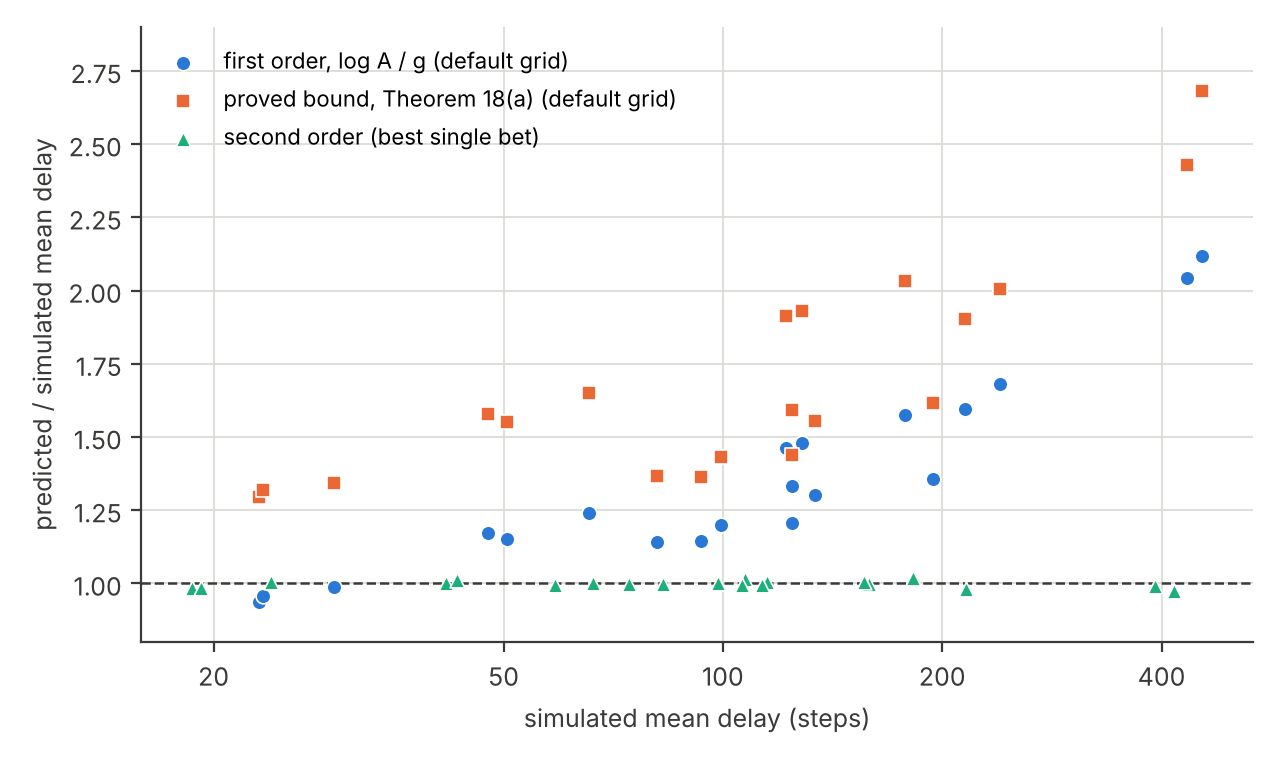
\includegraphics{figures/delay_predictions.png}
\caption{Figure S1. Simulated data. Ratio of predicted to simulated mean
delay for the first-order formula, the proved bound of Theorem 24(a)
(both for the default grid) and the second-order formula (best single
bet), for the 20 cases of Table S2.}
\end{figure}

\hypertarget{s5.-details-for-section-6-truncation-constant-slack-of-the-bound-delays-competitors-and-the-confidence-sequence-baseline}{%
\subsection{S5. Details for Section 6: truncation constant, slack of the
bound, delays, competitors and the confidence-sequence
baseline}\label{s5.-details-for-section-6-truncation-constant-slack-of-the-bound-delays-competitors-and-the-confidence-sequence-baseline}}

\textbf{The truncation constant.} For increases on clean data the delay
barely changes for \(c \ge 4\), and \(c = 3\) costs 3\%, 6\% and 12\% at
sd ratios 1.25, 1.5 and 2 against no truncation. With jumps (probability
0.005 per step, standard deviation 8 times the diffusive one) the growth
at sd ratio 1.25 peaks at \(c\) between 3.25 and 4.25 depending on the
change size, and without truncation it falls to 29\% of the \(c = 3\)
value. A burst of jumps at constant volatility (jump probability raised
from 0.005 to 0.02) moves the \(c = 3\) detector only 3.5\% as much as a
real 25\% volatility increase, against 39\% without truncation. For
decreases the speed limit dominates and a smaller \(c\) is usually
faster: with the true baseline and Gaussian data, \(c = 2\) shortens the
mean decrease delay by 26\% to 49\% relative to \(c = 3\). The two sides
need not share \(c\): with a known baseline, or with the
confidence-sequence baseline, which the monitor supports for the split
by running the lower bound on \(\min(r^2, \tau_{\downarrow}^2)\) and the
upper bound on \(\min(r^2, \tau^2)\), each at level \(\delta/2\), each
side is a valid e-detector for its own truncated statistic and the
two-sided rule of Proposition 5 needs only each side's guarantee, so
\(c\) of about 3 to 4 for increases and 1.5 to 2 for decreases is a
legitimate design. The decrease null then concerns the mean of
\(\min(r^2, \tau_{\downarrow}^2)\) for the smaller level
\(\tau_{\downarrow}\); volatility that has not fallen implies it under a
fixed innovation shape (Lemma 1), but a smaller clip reacts more to
changes of shape at constant volatility, such as a larger share of zero
returns. In the experiments the split was run with a 1440-step plug-in
baseline, which no proof covers: over all 18 no-change cells the one-day
rate was 5.0\% to 6.7\%, and 5.0\% to 6.05\% with
\(c_{\downarrow} = c\), so the excess over the 5\% bound that holds with
the true baseline is there without the split and comes from the
baseline. Table S3 gives the median decrease delays. For the Gaussian
law the split was also run with the confidence-sequence baseline
(\(\delta = 0.01\), \(A = 36{,}000\), two confidence sequences at
\(\delta/2\) when \(c_{\downarrow} \ne c\), on the same paths): its
one-day null rate was at most 0.05\% for \(c_{\downarrow}\) = 3, 2 and
1.5, against 5.65\% to 6.10\% for the plug-in, and its median decrease
delays were 24\% to 142\% longer (446.5 against 247 steps at a 20\% fall
with \(c_{\downarrow} = 3\)); \(c_{\downarrow} = 2\) was still faster
than \(c_{\downarrow} = 3\) in all three cells, and
\(c_{\downarrow} = 1.5\) was the fastest for falls to 0.67 and 0.5 times
but slower than \(c_{\downarrow} = 3\) for a 20\% fall (by 45 steps in
mean delay, standard error 9.8), where with the plug-in it was faster.
Rounded prices use a tick fixed in units of the pre-change standard
deviation, so that more returns are zero after a fall (at a tick of 0.5
standard deviations, 19.7\% before the change and 24.5\%, 29.1\% and
38.3\% after falls to 0.8, 0.67 and 0.5 of the standard deviation); a
first version of the experiment let the tick shrink with volatility and
overstated the gain.

\begin{longtable}[]{@{}
  >{\raggedright\arraybackslash}p{(\columnwidth - 6\tabcolsep) * \real{0.2500}}
  >{\raggedright\arraybackslash}p{(\columnwidth - 6\tabcolsep) * \real{0.2500}}
  >{\raggedright\arraybackslash}p{(\columnwidth - 6\tabcolsep) * \real{0.2500}}
  >{\raggedright\arraybackslash}p{(\columnwidth - 6\tabcolsep) * \real{0.2500}}@{}}
\toprule\noalign{}
\begin{minipage}[b]{\linewidth}\raggedright
Returns (calibration scale)
\end{minipage} & \begin{minipage}[b]{\linewidth}\raggedright
sd × 0.8: \(c_{\downarrow}\) = 3 / 2 / 1.5
\end{minipage} & \begin{minipage}[b]{\linewidth}\raggedright
sd × 0.67
\end{minipage} & \begin{minipage}[b]{\linewidth}\raggedright
sd × 0.5
\end{minipage} \\
\midrule\noalign{}
\endhead
\bottomrule\noalign{}
\endlastfoot
Gaussian & 247 / 176 / 185 & 158 / 85 / 73 & 118 / 58 / 40 \\
Student \(t_4\) & 334 / 289 / 277 & 160 / 117 / 106 & 100 / 62 / 48 \\
Jumps & 273 / 196 / 206 & 161 / 88 / 74 & 119 / 59 / 40 \\
Ticks of 0.25 sd (scale 1.11) & 292 / 185 / 188 & 191 / 98 / 77 & 144 /
69 / 45 \\
Ticks of 0.5 sd (scale 0.74) & \textbf{188 / 211 / 251} & 99 / 80 / 86 &
70 / 39 / 35 \\
Ticks of 0.75 sd (scale 1.11) & 295 / 201 / 207 & 192 / 100 / 81 & 144 /
69 / 47 \\
\end{longtable}

\emph{Table S3. Simulated data. Median decrease delay in steps with a
separate decrease clip \(c_{\downarrow}\) and \(c = 3\) for increases,
plug-in baseline from 1440 steps, \(A = 28{,}800\), change at the first
monitored step; 600 paths per cell for the continuous laws and 2000 for
rounded prices, the same paths for the three values of
\(c_{\downarrow}\); every path detected. ``Scale'' is the median
calibration scale (scaled MAD) in units of the true pre-change standard
deviation.}

With \(c_{\downarrow} = 2\) the median delay fell in all nine cells of
the continuous laws, by 13\% to 51\% (for Gaussian data the mean delay
fell by 25\%, 44\% and 50\%, close to the 26\%, 43\% and 49\% that the
theory predicts with the true baseline), and in all six cells with ticks
of 0.25 and 0.75 standard deviations, by 32\% to 52\%. At a tick of 0.5
standard deviations it was 12\% slower for a 20\% fall (median 211
against 188 steps; paired difference of 29 steps, standard error 1.7;
slower on 66\% of paths) and faster for larger falls, by 19\% and 44\%.
\(c_{\downarrow} = 1.5\) was no better than \(c_{\downarrow} = 2\) for a
20\% fall except under Student \(t_4\) returns, and at the tick of 0.5
standard deviations it was 34\% slower than \(c = 3\). A reading of the
tick case, not a proof: with rounded returns the calibration scale is,
on almost every path, a whole number of ticks times 1.4826, so at a tick
of 0.5 standard deviations it is 0.74 standard deviations against 1.11
at ticks of 0.25 and 0.75; \(c = 3\) then already clips at about 2.2
standard deviations, near the best clip for a 20\% fall, and
\(c_{\downarrow} = 2\) at about 1.5, past it, while the growing share of
zero returns after the fall adds to the effect. On the five
cryptocurrencies of Section 7, which have few zero returns (1.0\% to
4.3\% of deseasonalised returns), the choice \(c_{\downarrow} = 2\) was
neutral to slightly positive for the confirmation rate of decrease
alarms, within sampling noise. On data with a coarse tick,
\(c_{\downarrow} = 2\) should be compared with \(c = 3\) at that tick
before it is used.

\textbf{The slack of the false alarm bound.} An exact optional stopping
identity locates the slack by writing the ratio of the false alarm rate
to \(m/A\) as a product of a stopping factor, the share \(F_2\) of
expected wealth held on paths that crossed \(A\), and an overshoot
factor \(F_3\). For the default two-sided monitor (40,000 paths, rate
1.03\%) the stopping factor is close to 1, \(F_2 = 0.24\) and
\(F_3 = 0.80\): the slack is overshoot (a factor of 1.25) times wealth
stranded on paths that never alarm (a factor of about 4). Of the
stranded wealth, 60\% is held by the decrease side and 31\% by the three
smallest increase bets, which build little wealth within a day on
Gaussian data. The split of the budget between the two sides costs
almost nothing (both sides alarm on the same day in 0.00\% of days). The
bound itself is nearly sharp: for a single increase bet of 0.5, dynamic
programming over the whole nonparametric null finds a law with a one-day
false alarm rate of 4.73\%, 95\% of the bound, against 3.52\% for
Gaussian data. For the default mixture the best i.i.d. law found reaches
42\% of the bound for the increase grid alone, and an adaptive law
reaches 52\% for the two-sided detector (companion note); a certified
sharper bound for mixtures is open. Provable gains are possible by
splitting the budget unevenly between the sides and by dropping bets
that cannot use it.

Table S4 gives the false alarm rates with the true baseline behind
Figure 1 (left).

\begin{longtable}[]{@{}
  >{\raggedright\arraybackslash}p{(\columnwidth - 10\tabcolsep) * \real{0.1667}}
  >{\raggedright\arraybackslash}p{(\columnwidth - 10\tabcolsep) * \real{0.1667}}
  >{\raggedright\arraybackslash}p{(\columnwidth - 10\tabcolsep) * \real{0.1667}}
  >{\raggedright\arraybackslash}p{(\columnwidth - 10\tabcolsep) * \real{0.1667}}
  >{\raggedright\arraybackslash}p{(\columnwidth - 10\tabcolsep) * \real{0.1667}}
  >{\raggedright\arraybackslash}p{(\columnwidth - 10\tabcolsep) * \real{0.1667}}@{}}
\toprule\noalign{}
\begin{minipage}[b]{\linewidth}\raggedright
Horizon \(m\) (steps)
\end{minipage} & \begin{minipage}[b]{\linewidth}\raggedright
bound \(m/A\)
\end{minipage} & \begin{minipage}[b]{\linewidth}\raggedright
Gaussian
\end{minipage} & \begin{minipage}[b]{\linewidth}\raggedright
Student \(t_3\)
\end{minipage} & \begin{minipage}[b]{\linewidth}\raggedright
jumps
\end{minipage} & \begin{minipage}[b]{\linewidth}\raggedright
price ticks
\end{minipage} \\
\midrule\noalign{}
\endhead
\bottomrule\noalign{}
\endlastfoot
98 & 1.3\% & 0.00\% & 0.18\% & 0.12\% & 0.05\% \\
390 & 5.0\% & 1.1\% & 1.4\% & 1.3\% & 1.4\% \\
1950 & 25\% & 12.8\% & 14.3\% & 13.2\% & 13.7\% \\
3900 & 50\% & 29.6\% & 30.6\% & 29.7\% & 31.2\% \\
7800 & 100\% & 55.9\% & 55.9\% & 56.4\% & 56.9\% \\
\end{longtable}

\emph{Table S4. Simulated data. False alarm rate within \(m\) steps with
the true baseline, two-sided rule, \(A = 7800\), 4000 paths per law;
Student \(t_3\) has an infinite fourth moment. 95\% intervals at one day
are about \(\pm 0.3\) points.}

\textbf{Bet design.} The quarticity estimator can enter the detector
through the bet. A plug-in bettor with
\(\lambda_t = (\hat\mu_t - 1)/(\hat v_t + (\hat\mu_t - 1)^2)\), where
\(\hat\mu_t\) and \(\hat v_t\) are kernel-weighted local mean and
variance of \(Y\) over the last 60 steps (so that the local second
moment is a truncated local quarticity), added with weight one half to
the grid, was slower than the grid alone in 14 of 18 cells, by up to
9\%. A computation of growth rates explains this negative result: the
quadratic approximation behind the bet makes it 1.4 to 4.4 times too
small for increases, and it keeps only 49\% to 94\% of the attainable
growth. A grid designed by minimising the worst-case ratio to the best
single bet over a range of changes (sd ratio 1.2 to 2 up, 0.5 to 0.85
down) and four tail shapes, \(\lambda \in \lbrace 0.16, 0.39 \rbrace\)
up and \(\lambda/\lambda_{\max} \in \lbrace 0.5, 0.85 \rbrace\) down,
was at least as fast as the default in all 48 validation cases in its
design range, by 0.4\% to 10.5\% (median 5\%), but up to 17\% slower for
small increases (sd ratio 1.1) under fat tails. A grid tuned on Gaussian
data alone was up to 18\% faster on Gaussian or jump data and up to 55\%
slower under Student \(t_3\) data. The gains from bet design are modest,
and tuning to one tail shape is risky.

\textbf{Delays in the designs of Table 2.} Table S5 gives the median
delays of Section 6.2 after a change 500 steps into monitoring.

\begin{longtable}[]{@{}
  >{\raggedright\arraybackslash}p{(\columnwidth - 6\tabcolsep) * \real{0.2500}}
  >{\raggedright\arraybackslash}p{(\columnwidth - 6\tabcolsep) * \real{0.2500}}
  >{\raggedright\arraybackslash}p{(\columnwidth - 6\tabcolsep) * \real{0.2500}}
  >{\raggedright\arraybackslash}p{(\columnwidth - 6\tabcolsep) * \real{0.2500}}@{}}
\toprule\noalign{}
\begin{minipage}[b]{\linewidth}\raggedright
Detector
\end{minipage} & \begin{minipage}[b]{\linewidth}\raggedright
Gaussian
\end{minipage} & \begin{minipage}[b]{\linewidth}\raggedright
jumps
\end{minipage} & \begin{minipage}[b]{\linewidth}\raggedright
Student \(t_5\)
\end{minipage} \\
\midrule\noalign{}
\endhead
\bottomrule\noalign{}
\endlastfoot
\emph{Increases, sd ratio 1.25, 1.5, 2} & & & \\
Robust e-detector (default grid) & 87, 35, 17 (\(\le\) 4.3\%) & 102, 36,
18 (\(\le\) 4\%) & 122, 49, 22 (3\%) \\
Robust e-detector, CUSUM type & 154, 51, 23 (\(\le\) 1\%) & 171, 52, 23
(\(\le\) 0.3\%) & 215, 72, 32 (\(\le\) 0.3\%) \\
E-detector on raw \(r_t^2\) & 84, 33, 15 (\(\le\) 4.3\%) & 246, 60, 23
(\(\le\) 5.3\%) & 134, 51, 21 (\(\le\) 4\%) \\
Gaussian likelihood-ratio e-detector & 78, 26, 10 (\(\le\) 5.3\%) & 61,
20, 9 (\textbf{74 to 78\%}) & 46, 10, 7 (\textbf{96 to 98\%}) \\
Page CUSUM & 64, 24, 10 (6 to 10\%) & 54, 20, 11 (\textbf{74 to 79\%}) &
50, 9, 6 (\textbf{97 to 99\%}) \\
\emph{Decreases, sd ratio 0.5, 0.67, 0.8} & & & \\
Robust e-detector (default grid) & 71, 92, 147 (\(\le\) 2\%) & 72, 98,
160 (1\%) & 68, 96, 168 (\(\le\) 3\%) \\
Gaussian likelihood-ratio e-detector & 23, 46, 104 (6 to 9\%) & 23, 49,
121 (3 to 7\%) & 29, 81, 282 (\(\le\) 2\%) \\
\end{longtable}

\emph{Table S5. Simulated data. Median delay in steps after a change at
step 500 of monitoring; in brackets, the share of paths with a false
alarm during the 500 steps before the change, with plug-in baselines
from 2000 steps. These shares cover 500 steps, not a day: with a known
baseline Theorem 4 would bound them by \(500/7800 = 6.4\%\) per side.
300 paths per cell. The decrease detector on raw \(r_t^2\) does not
exist (Section 3.3).}

\textbf{BOCPD and the two-window scan.} BOCPD of Section 6.2 uses a
Gaussian model in each regime. The scan compares the realised variance
of the \(k\) returns before and after each candidate time, dropping
returns above 4 times a local bipower scale; it is our own construction,
not the published test of Bibinger, Jirak and Vetter (2017). On clean
Gaussian data BOCPD took a median of 13 steps against the e-detector's
20 for a doubling of the standard deviation. With the
confidence-sequence baseline the e-detector's one-day false alarm rate
in the online comparison of Section 6.2 was 0.1\% with jumps and 0.0\%
with Student \(t_5\) returns. Offline, on windows of 2000 steps, the
scan with \(k\) = 50 or 125 found a 25\% increase in 6\% to 30\% of
windows against 100\% for the e-detector; the gap is window length, not
betting, since with \(k = 500\) the scan found 99\%. The e-detector
needs no comparison window and no change location, only a change-free
calibration stretch, and it runs online, at about 11 microseconds per
step against about 300 for BOCPD.

\textbf{Competitors calibrated for the data at hand: definitions.} All
rules see the same calibration window (2000 steps) and monitored stream.
The \emph{classical rules on the e-detector's statistic} use
\(Y_t = X_t/m_0\) with the plug-in \(\tau\) and \(m_0\). Page's
two-sided CUSUM is
\(G_t^{\uparrow} = \max(0, G_{t-1}^{\uparrow} + Y_t - 1 - k_\theta)\)
and
\(G_t^{\downarrow} = \max(0, G_{t-1}^{\downarrow} + 1 - Y_t - k_\theta)\),
with the reference value \(k_\theta\) of the Gaussian likelihood ratio
for a change of the variance by a factor \(\theta\)
(\(k_\theta = \theta\log\theta/(\theta - 1) - 1\) for \(\theta > 1\) and
\(1 - \theta\log\theta/(\theta - 1)\) for \(\theta < 1\)): ``small'' for
standard deviation ratios 1.25 and 0.8 (\(k_\theta\) = 0.240 and 0.207)
and ``medium'' for 1.5 and 0.67 (0.460 and 0.348). The \emph{calibrated
betting rule} is the e-detector's own Shiryaev-Roberts statistic with a
calibrated threshold in place of \(2A\). Thresholds come either from
20,000 clean Gaussian paths, for the e-detector's own first-day rate
(1.3\%) or for 5\%, or from a bootstrap of each path's calibration
window (1000 replicates of a resampled window and a resampled 390-step
stream, the threshold of each side being the \(1 - \alpha/2\) quantile
of the replicate maxima for a target \(\alpha\)), which assumes i.i.d.
returns but no law. The \emph{Student \(t\) BOCPD} has a Student \(t\)
observation model with \(\nu = 3\) and an unknown variance on a grid,
the prior and short-run window (\(w = 250\)) of Section 6.2, and a
threshold matched to the e-detector's rate on Gaussian paths. The
\emph{training-sample rules} use the calibration window as a training
sample of size \(n_{\mathrm{tr}}\) and the detector \(\Sigma_j\), the
sum of \(Z_t\) minus its training mean over the first \(j\) monitored
steps, with \(Z_t = r_t^2\) (the setting of the published procedure) or
\(Z_t = X_t\); they alarm when
\(\lvert\Sigma_j\rvert \ge c_H\,\hat\sigma\sqrt{n_{\mathrm{tr}}}\,(1 + j/n_{\mathrm{tr}})\,(j/(n_{\mathrm{tr}} + j))^{\gamma}\),
where \(\hat\sigma\) is a Bartlett long-run standard deviation of the
training \(Z\) (bandwidth 12), \(\gamma = 0.25\) and the critical value
\(c_H\) comes from simulation. This is the boundary of monitoring in
linear models of Horváth, Hušková, Kokoszka and Steinebach (2004),
applied to squared returns as in Horváth, Kokoszka and Zhang (2006);
asymptotic critical values for open-ended monitoring spend almost none
of their 5\% in the first day for \(\gamma \le 0.25\). A second
boundary, that of OLS-CUSUM monitoring in the R package strucchange
(Zeileis, Leisch, Hornik and Kleiber 2002), is a check of the type of
Chu, Stinchcombe and White (1996). The papers of Horváth, Hušková,
Kokoszka and Steinebach (2004), Horváth, Kokoszka and Zhang (2006), Chu,
Stinchcombe and White (1996) and Knoblauch, Jewson and Damoulas (2018)
could not be read in full (footnote 1 of the main text), so these rules
are of the type of the published procedures, not reproductions, and no
\(\beta\)-divergence BOCPD was run.

\textbf{False alarms of the calibrated competitors.} On 4000 fresh paths
per law (bootstrap rules on 2000), calibrated on Gaussian data, the
CUSUMs on \(X\) had 5.0\% to 8.2\% false alarms in the first day under
Student \(t_3\) and \(t_5\) returns (target 1.3\%) and 14\% to 22\%
(target 5\%), and the training-sample rule on \(r_t^2\) 10\% to 15\%
under Student \(t_3\) returns and jumps (targets 1.3\% and 5\%).
Per-path bootstrap thresholds gave 1.4\% to 2.2\% (target 1.3\%) and
4.9\% to 6.3\% (target 5\%) under the six i.i.d.-type laws,
significantly above target in 5 of these 24 cells (the CUSUM on \(X\) at
the 1.3\% target under Student \(t_3\) returns, jumps and price noise,
and both rules at the 5\% target under price noise), and the
training-sample rule on \(X\) held its rate under every i.i.d.-type law
(1.1\% to 1.6\% at a 1.3\% target). Under GARCH and slow stochastic
volatility every rule alarmed on most paths, the e-detector included;
the training-sample rules, whose long-run variance absorbs part of the
clustering, alarmed least (21\% to 52\% in the first day).

\textbf{Delays of the calibrated competitors.} In the design of Table S5
(1000 paths per law and factor, bootstrap rules on 500), at the
e-detector's Gaussian rate the calibrated betting rule detected
increases of the standard deviation by 25\%, 50\% and 100\% in 106, 41
and 20 steps (e-detector 100, 39 and 19; here each side of the
e-detector alarms at \(2A\), against \(A\) in Table S5) and a fall to
0.8 times in 144 steps (e-detector 162). The calibrated rule is slower
for increases although its false alarm rate before the change is higher
(3.2\% against 2.6\%), because it splits its target first-day rate
equally between the two sides, while the e-detector's realised first-day
rate falls mostly on the increase side; Page's CUSUM on \(X\) was as
fast for increases and 15\% to 40\% faster for decreases. Against
thresholds that spend the full 5\% in the first day, at 4.5\% to 4.9\%
first-day false alarms, the e-detector took 1.1 to 1.3 times as long for
increases and 1.4 to 2.1 times for decreases, and such thresholds hold
only if the law is known. With bootstrap thresholds under Student
\(t_3\) returns the e-detector detected increases 16\% to 24\% faster
than the CUSUM, and the CUSUM decreases 3\% to 10\% faster. The
training-sample rules were about twice as slow: on \(r_t^2\) at the
matched Gaussian rate 199, 82 and 35 steps for increases and 330, 204
and 140 for decreases. This is a property of the boundary: \(\Sigma_j\)
accumulates the departure from the training mean since monitoring began,
and with \(c_H = 1.83\), \(\hat\sigma = \sqrt 2\) (Gaussian \(r_t^2\))
and \(n_{\mathrm{tr}} = 2000\) the boundary is about 104 squared-return
units at \(j = 600\), so an increase of the variance by 0.5625 per step
(standard deviation ratio 1.25) needs about 185 steps after the change,
plus the growth of the boundary meanwhile, while Page's CUSUM and the
e-detector restart their evidence whenever it turns against a change.

\textbf{The Student \(t\) BOCPD.} On the paths of the online comparison
of Section 6.2 it had 0.7\% false alarms in the first day under jumps
and 3.3\% under Student \(t_5\) returns, against 73.2\% and 53.2\% for
the Gaussian BOCPD, but 4.9\% under Student \(t_3\) and 0.5\% under
Gaussian data with the same threshold; within 1500 steps it found only
56\% of 25\% increases and 77\% of 20\% decreases (e-detector 98\%),
while it was faster for halvings of the standard deviation (27 against
81 steps).

\textbf{Width of the confidence-sequence baseline.} From 292
observations its median upper bound sits 37\% above the true mean for
Gaussian returns, against 29\% for the best constant bet for the true
law, a benchmark that knows the distribution; at 1440 steps and more it
is within 3.5 points of that benchmark.

\textbf{Delays with the confidence-sequence baseline.} The false alarm
check of Section 6.3 used three laws, calibration of 390, 1440 and 5000
steps, and 10,000 paths in each of the nine settings. Table S6 gives the
median delays of Section 6.3.

\begin{longtable}[]{@{}
  >{\raggedright\arraybackslash}p{(\columnwidth - 6\tabcolsep) * \real{0.2500}}
  >{\raggedright\arraybackslash}p{(\columnwidth - 6\tabcolsep) * \real{0.2500}}
  >{\raggedright\arraybackslash}p{(\columnwidth - 6\tabcolsep) * \real{0.2500}}
  >{\raggedright\arraybackslash}p{(\columnwidth - 6\tabcolsep) * \real{0.2500}}@{}}
\toprule\noalign{}
\begin{minipage}[b]{\linewidth}\raggedright
Returns, sd ratio
\end{minipage} & \begin{minipage}[b]{\linewidth}\raggedright
390 steps: plug-in / CS
\end{minipage} & \begin{minipage}[b]{\linewidth}\raggedright
1440 steps: plug-in / CS
\end{minipage} & \begin{minipage}[b]{\linewidth}\raggedright
5000 steps: plug-in / CS
\end{minipage} \\
\midrule\noalign{}
\endhead
\bottomrule\noalign{}
\endlastfoot
Gaussian, 1.25 & 90 / 645 (76\%) & 88 / 222 & 88 / 134 \\
Gaussian, 1.5 & 36 / 103 & 35 / 59 & 35 / 46 \\
Gaussian, 2 & 17 / 31 & 17 / 24 & 17 / 20 \\
Gaussian, 0.8 & 143 / 633 (85\%) & 137 / 269 & 139 / 199 \\
Gaussian, 0.67 & 89 / 207 & 87 / 135 & 87 / 114 \\
Gaussian, 0.5 & 64 / 122 & 65 / 92 & 64 / 80 \\
Student \(t_5\), 1.25 & 128 / 904 (35\%) & 131 / 391 & 130 / 219 \\
\end{longtable}

\emph{Table S6. Simulated data. Median delay in steps after a change at
step 500, plug-in against confidence-sequence (CS) baseline, by
calibration length, 2000 paths per cell. Medians are over the paths that
detected the change within 2500 steps; where the share detected (in
brackets, shown when below 90\%) is low, the CS median is biased
downwards. With 390 calibration steps the plug-in detects only 92\% to
94\% of increases in this sense, because it alarms before the change on
6\% to 7.5\% of paths.}

\hypertarget{s6.-clustering-forecasts-the-garch-bound-and-price-noise}{%
\subsection{S6. Clustering, forecasts, the GARCH bound and price
noise}\label{s6.-clustering-forecasts-the-garch-bound-and-price-noise}}

\textbf{Volatility clustering.} Under GARCH(1,1) returns with constant
unconditional variance, the conditional mean of \(X_t\) moves above and
below \(m_0\), so the nulls of Section 2 are false. With the true
unconditional baseline and \(A = 28{,}800\) for a 1440-step day, the
share of days with an alarm is 78\% at persistence
\(\alpha + \beta = 0.95\) (half-life 14 steps) and 100\% at 0.99, 0.999
and 0.9999 (Figure 1, right). A band \(b = 0.5\) absorbs short-lived
clustering (3.6\% at persistence 0.95), but no reasonable static band
absorbs persistent clustering: even \(b = 1\) on the increase side
leaves 12\% to 20\% of days with an alarm at persistence 0.99 or more.
For slow log-normal stochastic volatility (log-sd 0.15, half-life 390
steps), whose first-day alarm rates at band 0 were 24.7\% (increase) and
26.7\% (decrease), a band of 0.25 brought them to 8.3\% and 5.0\% while
90\% of doublings and 94\% of halvings of volatility were still detected
(68\% and 66\% at band 0, where false alarms often came first), with
median delays of 28 and 111 steps against 19 and 74 at band 0, and a
band of 0.5 to 1.7\% and 0.0\% with 97\% and 100\% detected; the band is
a design choice, not a guarantee. These alarms are not errors of the
proof: persistent GARCH clusters are changes in conditional volatility,
and the monitor reports them.

\textbf{Forecast-relative monitoring.} Monitoring \(r_t/\hat\sigma_t\)
with a GARCH(1,1) forecast fitted on a separate path and then frozen
brings the one-day false alarm rate down to 3.0\% to 6.2\% at all three
persistences (600 paths, plug-in baseline from one day), the level of
the oracle with the true conditional volatility and the same plug-in
baseline (4.7\% to 5.3\%). This is not a proved guarantee: the proof
needs the true or a confidence-sequence baseline and a correct forecast
model, and with the true baseline the one-day rate for i.i.d. returns is
1.1\% to 1.4\%, so the plug-in roughly quadruples it. An EWMA forecast
is only as valid as its match to the clustering (half-life 360 steps:
72\% to 100\% at band 0). The price is the bound of Proposition S13
below. At persistence 0.99, a doubling of the long-run variance was
detected within one day on 34\% to 43\% of paths and within five days on
93\% to 94\%, with median delays of 1523 to 1791 steps; without a break
the same monitors alarmed within one day on 4\% to 6\% and within five
days on 38\% to 44\% of paths, the latter far above the 25\% that
Theorem 4 guarantees with a known baseline. A fourfold increase of the
long-run variance was detected within a day on 89\% to 90\% of paths
(median 612 to 712 steps). For the oracle, whose standardised returns
are exactly i.i.d., the excess over five days is the plug-in effect of
Section 4.1, not a property of the forecast.

\textbf{Price-level microstructure noise.} With i.i.d. noise on log
prices, \(\mathbb{E}[r_t^2 \mid \mathcal{F}_{t-1}]\) depends on the last
noise value, so squared returns are positively autocorrelated and the
null fails without any change in volatility. At one-second sampling
(23,400 steps per day, \(A\) set to give 5\% for the first day, plug-in
baseline from two days) the one-day false alarm rate of the increase
side on raw returns rose from 5.0\% without noise to 8.5\%, 18.0\%,
31.0\% and 41.5\% at noise-to-signal ratios 0.5, 1, 2 and 4 (200 days
per cell); overlapping pre-averaged returns alarmed on every day,
because consecutive windows share most of their prices. Pre-averaging
over non-overlapping blocks of prices, skipping the one return between
blocks, gives each block fresh noise values, so the null holds for the
block statistic whenever the spot variance and the noise law are
unchanged, and Theorems 3 and 4 apply to it for every block of
\(n_{\mathrm{b}} \ge 2\) prices; the block monitors were below the bound
or within Monte Carlo error of it in all 58 cells tested, and with
\(n_{\mathrm{b}} = 10\) were about 8 times slower than raw returns
without noise and faster than them from a noise ratio of about 2.
One-minute crypto returns were not tested for noise of this kind; the
effect is largest at the highest frequencies.

\textbf{Proposition S13 (a bound on the ratio of means after a break).}
Let \(\alpha, \beta > 0\) with \(\alpha + \beta < 1\) and
\(\omega > 0\). Before a break the returns follow
GARCH\((\omega, \alpha, \beta)\), and the forecast is the pre-break
filter \(s_t = \omega + \alpha r_{t-1}^2 + \beta s_{t-1}\), run without
change after the break. From the break on, the returns follow
GARCH\((\theta\omega, \alpha, \beta)\) with \(\theta > 0\):
\(r_t = \sigma_t \varepsilon_t\),
\(\sigma_t^2 = \theta\omega + \alpha r_{t-1}^2 + \beta \sigma_{t-1}^2\),
with i.i.d. \(\varepsilon_t\) of mean 0 and variance 1. Then
\(\Delta_t = \sigma_t^2 - s_t\) satisfies
\(\Delta_t = (\theta-1)\omega + \beta \Delta_{t-1}\) deterministically,
so \(\Delta_t \to (\theta-1)\omega/(1-\beta)\) geometrically at rate
\(\beta\), and in the post-break stationary regime \[
\rho(\theta) := \frac{\mathbb{E}[r_t^2]}{\mathbb{E}[s_t]} = \frac{\theta(1-\beta)}{1 - \alpha - \beta + \alpha \theta},
\] which does not depend on \(\omega\), increases in \(\theta\), and
satisfies \(\rho(\theta) < (1-\beta)/\alpha\) for every \(\theta\),
however large the break.

\emph{Proof.} Subtracting the two recursions, the terms
\(\alpha r_{t-1}^2\) cancel, which gives the recursion for \(\Delta_t\).
In the post-break stationary regime
\(\mathbb{E}[r_t^2] = \mathbb{E}[\sigma_t^2] = \theta\omega/(1 - \alpha - \beta)\)
and
\(\mathbb{E}[s_t] = \mathbb{E}[\sigma_t^2] - (\theta-1)\omega/(1-\beta)\).
Dividing and simplifying gives \(\rho(\theta)\). Its derivative in
\(\theta\) has the sign of \((1-\beta)(1-\alpha-\beta) > 0\), and
\(\rho(\theta) \to (1-\beta)/\alpha\) as \(\theta \to \infty\).
\(\square\)

Proposition S13 is the mirror image of the finding that unmodelled
shifts make GARCH fits look nearly integrated (Diebold 1986; Lamoureux
and Lastrapes 1990; Mikosch and Starica 2004). Two exact facts sit
behind it. A scale break (\(r_t \mapsto \sqrt{\theta}\, r_t\)) and an
intercept break (\(\omega \mapsto \theta\omega\)) lead to the same
post-break model and differ only in the transient right after the break.
And the filter absorbs most of the break through its \(\alpha r^2\)
term: at persistence \(\alpha + \beta = 0.99\) with \(\alpha = 0.05\), a
doubling of the long-run variance appears after standardisation as an
increase of the ratio of means to \(\rho(2) = 1.091\), and no break can
push it above \((1 - \beta)/\alpha = 1.2\). Here \((1-\beta)/\alpha\)
bounds the post-break ratio of the mean squared return to the mean
forecast; it is not a fraction of the shift. The monitor sees the mean
of the ratio, \(\mathbb{E}[r_t^2/s_t]\), which is a little larger by
Jensen's inequality (1.116 for \(\theta = 2\) in simulation) and which
stayed below 1.28 for \(\theta\) up to 1000 at this persistence. At
persistence 0.95 and \(\theta = 1000\) the mean of the ratio, 2.20,
exceeds the bound 2.0 on the ratio of means, so the bound does not cover
the quantity the monitor sees; we have a proof only for the ratio of
means. Figure S2 compares the closed form with simulation: the simulated
ratio of means, pooled over paths, agrees with \(\rho(\theta)\) within
two standard errors at every point. (An average of per-path ratios is
biased upward when the path means are noisy; at persistence 0.999 it
exceeded the bound, which is why we pool.)

\begin{figure}
\centering
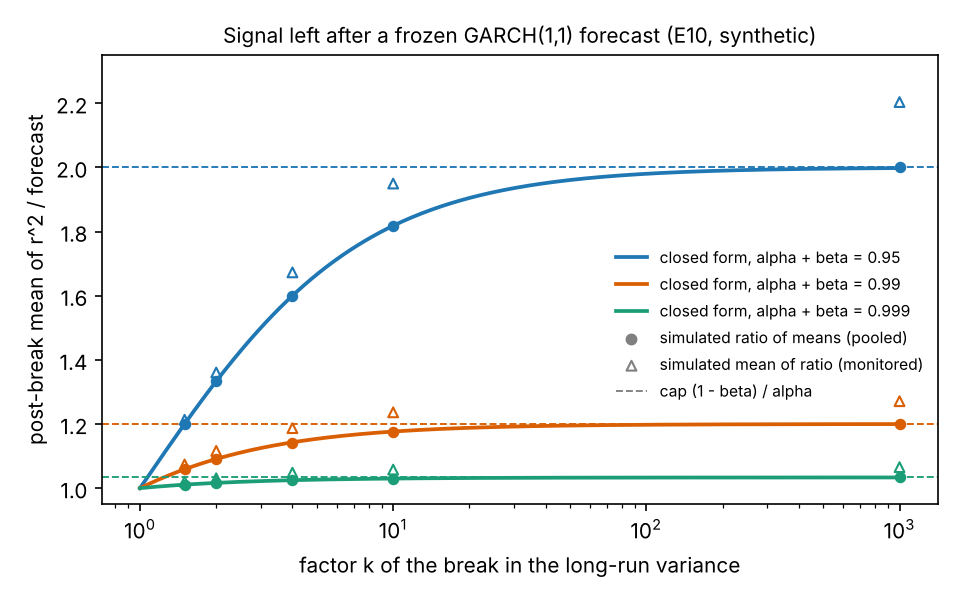
\includegraphics{figures/signal_cap.png}
\caption{Figure S2. Simulated data. The ratio of means \(\rho(\theta)\)
after a break of factor \(\theta\) in the long-run variance (lines,
closed form; filled markers, simulation pooled over paths, with bars of
two bootstrap standard errors) and the mean of the ratio that the
monitor sees (open triangles), with the bounds \((1-\beta)/\alpha\) on
the ratio of means (dashed), for three persistences. The mean of the
ratio is not covered by the bound and exceeds it at persistence 0.95 for
large breaks. 200 paths of 18,000 post-break steps per point; all
standard errors are below 0.002.}
\end{figure}

\textbf{An information rate.} With Gaussian innovations the per-step
Kullback-Leibler divergence between the post-break and pre-break
conditional laws of \(r_t\) is \(\tfrac12(q_t - 1 - \ln q_t)\) with
\(q_t = \sigma_t^2/s_t\). Let \(I\) be its average over the post-break
path. By Lai (1998), any detector whose average run length to a false
alarm is at least \(A\) needs, as \(A \to \infty\) and under his
condition that the post-change log-likelihood ratio grows at rate \(I\)
uniformly in the change time, a worst-case delay of at least
\((\ln A/I)(1 + o(1))\). At \(A = 28{,}800\) this is an
order-of-magnitude guide, not an exact bound. Table S7 gives the
numbers.

\begin{longtable}[]{@{}
  >{\raggedright\arraybackslash}p{(\columnwidth - 10\tabcolsep) * \real{0.1667}}
  >{\raggedright\arraybackslash}p{(\columnwidth - 10\tabcolsep) * \real{0.1667}}
  >{\raggedright\arraybackslash}p{(\columnwidth - 10\tabcolsep) * \real{0.1667}}
  >{\raggedright\arraybackslash}p{(\columnwidth - 10\tabcolsep) * \real{0.1667}}
  >{\raggedright\arraybackslash}p{(\columnwidth - 10\tabcolsep) * \real{0.1667}}
  >{\raggedright\arraybackslash}p{(\columnwidth - 10\tabcolsep) * \real{0.1667}}@{}}
\toprule\noalign{}
\begin{minipage}[b]{\linewidth}\raggedright
\(\alpha + \beta\)
\end{minipage} & \begin{minipage}[b]{\linewidth}\raggedright
\(\theta\)
\end{minipage} & \begin{minipage}[b]{\linewidth}\raggedright
\(\rho(\theta)\)
\end{minipage} & \begin{minipage}[b]{\linewidth}\raggedright
simulated mean of ratio
\end{minipage} & \begin{minipage}[b]{\linewidth}\raggedright
\(I\) (nats per step)
\end{minipage} & \begin{minipage}[b]{\linewidth}\raggedright
\(\ln A / I\) (days of 1440 steps)
\end{minipage} \\
\midrule\noalign{}
\endhead
\bottomrule\noalign{}
\endlastfoot
0.95 & 2 & 1.333 & 1.361 & 0.028 & 0.26 \\
0.99 & 1.5 & 1.059 & 1.074 & 0.0015 & 4.7 \\
0.99 & 2 & 1.091 & 1.116 & 0.0037 & 1.9 \\
0.99 & 4 & 1.143 & 1.187 & 0.0093 & 0.77 \\
0.99 & 1000 & 1.200 & 1.271 & 0.019 & 0.38 \\
0.999 & 2 & 1.016 & 1.031 & 0.00033 & 21.4 \\
\end{longtable}

\emph{Table S7. Simulated data. Signal left after a frozen GARCH(1,1)
forecast and the information rate of a break, \(A = 28{,}800\); \(I\) to
two significant figures.}

The observed median delays of the forecast-relative monitors (1523 to
1791 steps for a doubling, Section 6.4) are about 0.6 times the step at
which the cumulative information reaches \(\ln A\); the memory term of
Section 5.3 can explain a factor of this size on its own (in an i.i.d.
version of the same steady state with the true baseline the detector
alarms at 0.41 to 0.58 times \(\ln A/\mathrm{KL}\)), but we did not
rerun the GARCH setting to separate it from the effect of the plug-in
baseline.

\hypertarget{s7.-real-data-details}{%
\subsection{S7. Real-data details}\label{s7.-real-data-details}}

\hypertarget{s7.1-the-nifty-50-index-and-india-vix}{%
\subsubsection{S7.1 The Nifty 50 index and India
VIX}\label{s7.1-the-nifty-50-index-and-india-vix}}

\textbf{Data.} Nifty 50 one-minute bars from April 2017 to October 2026,
sessions of 375 bars, overnight returns excluded. Stretches of five or
more minutes with a frozen index value (exchange outages, the two
market-wide halts of March 2020, and the closing auction minutes from 3
August 2026) were set to missing, leaving 2,361 sessions and 882,001
returns. The intraday profile is session-aware, so that the close is not
smoothed into the open. Pre-registered configuration: calibration 750
bars, band 0.25; development period 2017 to 2021, held-out period 2022
to October 2026, with nothing changed after the held-out period was
seen. A configuration was pre-registered, not a primary test, so the
results below are secondary.

\textbf{Results.} The monitor raised 0.26 alarms per session in both
periods. In the held-out period, 78\% of increase alarms were followed
by a session more volatile than the baseline (47\% at random times) and
76\% of decrease alarms by a calmer one (53\%), with 95\% intervals of
72\% to 84\% and 69\% to 82\% from a block bootstrap over sessions
(blocks of 5 sessions; Holm \(p = 0.0008\)); the Gaussian
likelihood-ratio monitor's increase alarms were followed by higher
volatility only 61\% of the time, while its decrease alarms were as
informative. India VIX agreed with the alarms on the same day (in the
development years VIX closed higher on 68\% of days with an increase
alarm, against 47\% of all days), which holds after Holm over eight
comparisons in the development years and for decrease alarms in the
held-out years, but not for held-out increase alarms (Holm
\(p = 0.25\)). VIX did not move in the alarm's direction on the next day
more often than on other days (45\% to 48\% against 46\% to 47\%): the
agreement is concurrent, not a lead. The event analysis below was not
part of the pre-registered configuration. Among event days, 9 of 11
Union Budget sessions had an alarm, against 25\% of ordinary sessions
(Fisher \(p = 0.0001\); Holm over the five event types 0.0006; a
circular-shift test of the event calendar against the alarm series,
which keeps the clustering of alarms, gives \(p = 0.0004\) and Holm
0.0021), and so did all 7 budget sessions at which the monitor was
already watching at the open, a restriction chosen after the first
results. Reserve Bank of India policy days showed no significant excess
(32\% against 25\%, \(p = 0.36\)), consistent with their volatility
being close to the recent norm (median 1.06 times the previous 20
sessions). Monthly derivative expiry days had more alarms (38\%,
\(p = 0.002\); Holm 0.0095, and 0.015 with the circular shift), which
may be an artefact of a profile that pools all weekdays. In March 2020
volatility was 2.7 times that of the previous 20 sessions, yet only 6 of
21 sessions had an alarm: after each alarm the monitor recalibrates on
the new, already high level. It answers ``has volatility changed from
the recent baseline?'', not ``is volatility high?''.

\hypertarget{s7.2-fomc-statements-and-cpi-releases}{%
\subsubsection{S7.2 FOMC statements and CPI
releases}\label{s7.2-fomc-statements-and-cpi-releases}}

\textbf{Design.} Binance BTC, ETH and SOL from 21 January 2024 to 31
December 2025; the 16 FOMC rate decisions (statement at 14:00 US
Eastern) and 22 US CPI releases (08:30 US Eastern) of 2024 and 2025
inside the monitored period, with every date checked against a published
schedule. Control windows are all days at least two days away from any
event day, with the same weekday, at the same Eastern clock time (134
for FOMC, 299 for CPI); each event is compared with the control windows
of its own weekday, and the control rates below are these matched rates
averaged over events. The outcome is an increase alarm within six hours
of the anchor, and the test is a stratified permutation test, exact when
the strata are independent; releases of one weekday and clock time share
their control windows, which can raise its level slightly (5.8\% at a
nominal 5\% for seven FOMC statements in the simulation of the test on
fresh releases below). The primary family is FOMC and CPI on BTC in the
streaming design (the monitor as a user would have run it), with a Holm
correction; it is stated as fixed before the first run in the analysis
code, which was first saved together with the results. ETH and SOL are
secondary replications, and a design in which a fresh monitor is
calibrated on the day before every anchor was added after the streaming
results were seen and is exploratory.

\textbf{Results.} In the streaming design (the primary family), 9 of 16
FOMC statements on BTC were followed by an increase alarm within six
hours, against 14\% of control windows (Holm-adjusted \(p = 0.00025\));
the CPI test was not significant on BTC (5 of 22 against 12\%,
\(p = 0.11\)) but was significant on ETH (\(p = 0.003\)) and SOL
(\(p = 0.00004\); Holm within the replications 0.0032 and 0.00015). The
streaming monitor was recalibrating after its own alarms about 70\% of
the time and was awake at only 9 of the 16 FOMC statements on BTC; at
those it alarmed every time (and at 8 of 8 on ETH and 9 of 9 on SOL), a
restriction made after the first run. Exploratory from here on. With a
fresh calibration, 14 to 15 of the 16 FOMC statements raised an alarm
within six hours, against 29\% to 32\% of controls, and 59\% to 73\% of
CPI releases, against 23\% to 28\%. The alarms came after the release
(median 23 to 34 minutes, never before 14 minutes on BTC and SOL and 10
minutes on ETH), and there is no sign of more alarms in the hours before
a release. The Gaussian likelihood-ratio monitor with a fresh
calibration also alarmed at almost every release, but with a median
delay of 0 to 2 minutes, on a single return of 8 to 9 robust scale units
(median): one large minute is enough to trigger it. It also alarmed in
62\% to 76\% of control windows. Because it ran at band 0 and the robust
monitor at band 0.25, this contrast mixes the band with the truncation;
run at band 0 as well, the robust monitor with a fresh calibration
alarmed at 14 to 15 of 16 FOMC statements and 16 to 18 of 22 CPI
releases, with a median delay of 18 to 22 minutes, and in 39\% to 51\%
of control windows. The truncated detector cannot be moved by one minute
(one clipped observation multiplies its statistic by a bounded factor),
and its delays and the size of its largest recent return are those of a
short volatility regime; the share of release alarms classed as ``jump
only'' did not separate the two monitors, so this reading rests on the
delays and the return sizes.

\textbf{The rerun with proved monitors (pre-registered).} The rerun was
pre-registered before any of its real-data runs and keeps everything of
the design above except the monitor (Table S12). Primary: the
confidence-sequence baseline (\(\delta = 0.01\), \(A = 36{,}000\), band
0.25) restarted at 00:00 UTC, with a 1440-minute recalibration after
each alarm, so that each UTC day is one period of Corollary S14 and the
monitor raises at most one alarm a day; its bound, 5\% for each day of a
segment, is marginal and needs the tolerance during that day. Secondary:
the same without the restart (5\% for the first day of each segment) and
the rank detector restarted without a blind period, with payoffs divided
by 1.25 (Theorem S16). In the primary family (BTC, Holm over FOMC and
CPI), 8 of 16 FOMC statements were followed by an up alarm within six
hours against 10.9\% of matched controls (\(p = 0.00017\), Holm
0.00033), and 5 of 22 CPI releases against 5.9\% (Holm 0.0097); the
plug-in had 9 of 16 against 13.9\% and 5 of 22 against 11.7\%, so for
CPI the count of releases is unchanged and the matched control rate
halved. Every FOMC cell held after Holm, on ETH and SOL, without the
restart and with the rank detector; CPI did not hold on ETH and SOL
under the primary monitor (Holm 0.075) or without the restart on BTC (3
of 22, \(p = 0.12\)) and SOL. The rank detector's cells repeat an
earlier run exactly and add no confirmatory evidence, and the plug-in
run through the same code reproduced the results above exactly. The
primary monitor watched 80 of the 114 coin and release pairs (without
the restart 77, the rank detector 114, the plug-in 55); one BTC FOMC
statement (29 January 2025) fell in a segment whose increase side could
not alarm. It alarmed on 48.1\% to 53.5\% of the UTC days on which it
monitored at least one minute and raised 0.92 to 1.15 alarms per 1440
monitored minutes, against a long-run bound of 0.0404 per 1440 monitored
minutes under the tolerance (Corollary 18 and the remark after its
proof), so the tolerance fails on many of these days and the rerun does
not test the bound. The restart at 00:00 UTC falls five hours into the
six-hour window of FOMC statements made in US Eastern standard time. The
data and the plug-in results were known when the rerun was designed, and
16 statements give a wide interval (28\% to 72\% for the primary rate);
the contrast was not confirmed on the releases of 2026 (below).

\textbf{The test on fresh releases (pre-registered).} The
pre-registration was committed with the event file before any Binance
return of 2026 was downloaded. Releases: the FOMC statements (14:00 US
Eastern) and CPI releases (08:30 US Eastern) of 2026 whose six-hour
window ends before the data end, 24 October 2026 23:59 UTC, that is 6
FOMC statements (28 January to 16 September; that of 28 October is
excluded) and 10 CPI releases (13 January to 14 October), each date
checked by web search against the Federal Reserve and BLS announcements.
Data: Binance BTC, ETH and SOL, monitored from 1 January 2026 for 297
days with no missing minute. Monitors, control windows (29 for each
release, 39 for releases on a Friday) and outcome are those of the
rerun. Primary: the confidence-sequence monitor restarted at 00:00 UTC
on BTC, with one one-sided stratified permutation test over all 16
releases that passes at \(p \le 0.05\); it was chosen over a test of the
FOMC statements alone because its power at the rerun's BTC rates was
0.82 against 0.69 for the 17 releases planned (0.78 against 0.62 for the
16 in the data, and 0.37 against 0.28 if the excess were half as large).
Result: 2 of 16 releases against 5.9\% of matched controls
(\(p = 0.25\), Fisher 0.29; Wilson interval 3.5\% to 36.0\%); the same
design on the releases of 2024 and 2025 gives 13 of 38 against 8.0\%.
Secondary families, Holm within each: this monitor pooled on ETH and
SOL, 4 and 5 of 16 (Holm 0.079 for both); its six FOMC and CPI cells,
none below Holm 0.48; the plug-in, one cell (ETH, FOMC, 4 of 6, Holm
0.040); the rank detector restarted without a blind period, 4 of 6 FOMC
statements on every coin (Holm 0.016, 0.033 and 0.055) and no CPI cell;
the monitor without the restart, no cell. On BTC the primary monitor was
recalibrating at 2 releases and unable to raise an increase alarm
(\(\tau^2 \le m^{\uparrow}\)) at 3, in two segments of 4.6 and 47.0 days
that held 28.0\% of its monitored time, and alarmed after 2 of the 11
releases it watched (13 of 26 in 2024 and 2025). It alarmed on 37.8\% to
48.0\% of the UTC days on which it monitored at least one minute,
against 5\% under the tolerance. With power 0.78, a failure has
probability about 0.22 if the rates of the rerun were true and about
0.63 if the excess were half as large, so the failure does not show that
there is no contrast. In the power simulation the stratified test of the
individual release types, which treats releases that share control
windows as independent strata, had level 5.8\% for seven FOMC statements
sharing 29 control windows (Monte Carlo standard error 0.17 points) and
4.7\% for six; the pooled test stayed below 5\%. Post hoc and
descriptive: the mean absolute return in the first hour after a BTC
release, relative to the six hours before, had medians of 2.11 (FOMC)
and 1.73 (CPI) in 2026, against 2.51 and 2.00 in 2024 and 2025.

\hypertarget{s7.3-forecasts-and-competitors-on-real-data}{%
\subsubsection{S7.3 Forecasts and competitors on real
data}\label{s7.3-forecasts-and-competitors-on-real-data}}

Table S8 gives the comparison with forecasts of Section 7.2 for the
plug-in baseline, with 95\% intervals from the block bootstrap over
calendar days of Section 7.1. The ratio rules alarm when the robust
volatility of the last 60 or 240 minutes, divided by that of the
preceding day, crosses thresholds chosen on the same data to give the
e-detector's numbers of up and down alarms, with the same dead time;
this hindsight favours them. With the hindsight-tuned ratio rule, the
one comparison that holds after Holm adjustment (band 0.5, out of
sample) has the e-detector's decrease alarms confirmed 10.5 points more
often than the 60-minute rule's (Holm \(p = 0.0096\)). Out of sample the
intervals of the differences lie within plus or minus 5 points in 7 of 8
cells at band 0.25, but in July to December 2025 they reach 9.7 points.

\begin{longtable}[]{@{}
  >{\raggedright\arraybackslash}p{(\columnwidth - 6\tabcolsep) * \real{0.2500}}
  >{\raggedright\arraybackslash}p{(\columnwidth - 6\tabcolsep) * \real{0.2500}}
  >{\raggedright\arraybackslash}p{(\columnwidth - 6\tabcolsep) * \real{0.2500}}
  >{\raggedright\arraybackslash}p{(\columnwidth - 6\tabcolsep) * \real{0.2500}}@{}}
\toprule\noalign{}
\begin{minipage}[b]{\linewidth}\raggedright
Rule
\end{minipage} & \begin{minipage}[b]{\linewidth}\raggedright
Period
\end{minipage} & \begin{minipage}[b]{\linewidth}\raggedright
Up alarms: next day above forecast
\end{minipage} & \begin{minipage}[b]{\linewidth}\raggedright
Down alarms: next day below forecast
\end{minipage} \\
\midrule\noalign{}
\endhead
\bottomrule\noalign{}
\endlastfoot
Random times (EWMA / HAR) & Jul to Dec 2025 & 49.4\% / 51.3\% & 50.6\% /
48.7\% \\
Robust e-detector (EWMA) & Jul to Dec 2025 & 78.5\% (72.0 to 84.5),
\(n = 367\) & 80.5\% (74.6 to 86.3), \(n = 256\) \\
Robust e-detector (HAR) & Jul to Dec 2025 & 80.7\% (74.7 to 86.4) &
78.1\% (70.3 to 85.5) \\
Ratio rule, 60 / 240 min (EWMA) & Jul to Dec 2025 & 73.9\% / 74.2\% &
78.1\% / 82.3\% \\
Random times (EWMA / HAR) & out of sample & 50.4\% / 48.3\% & 49.6\% /
51.7\% \\
Robust e-detector (EWMA) & out of sample & 77.1\% (73.5 to 80.5),
\(n = 951\) & 70.9\% (66.7 to 75.1), \(n = 870\) \\
Robust e-detector (HAR) & out of sample & 75.9\% (72.0 to 79.6),
\(n = 909\) & 73.6\% (69.9 to 77.3), \(n = 834\) \\
Ratio rule, 60 / 240 min (EWMA) & out of sample & 77.0\% / 75.7\% &
67.4\% / 70.9\% \\
\end{longtable}

\emph{Table S8. Market data, five coins pooled, band 0.25, plug-in
baseline. Share of alarms after which the next day's robust volatility
was on the flagged side of a forecast made at the alarm, with 95\%
intervals from the block bootstrap over calendar days of Section 7.1 in
brackets. The HAR rows out of sample have fewer alarms because the HAR
forecast needs a longer history.}

We repeated the comparison of Table S8 for BOCPD and the two-window
variance-ratio scan (inspired by Bibinger, Jirak and Vetter 2017) of
Section 6.2, run continuously with predictable priors and scales and
with the same one-day pause after every alarm, and with their up and
down thresholds set per series so that each raises as many up and down
alarms as the e-detector at band 0.25 (about 0.68 alarms per day). Table
S9 pools the five coins.

\begin{longtable}[]{@{}
  >{\raggedright\arraybackslash}p{(\columnwidth - 4\tabcolsep) * \real{0.3333}}
  >{\raggedright\arraybackslash}p{(\columnwidth - 4\tabcolsep) * \real{0.3333}}
  >{\raggedright\arraybackslash}p{(\columnwidth - 4\tabcolsep) * \real{0.3333}}@{}}
\toprule\noalign{}
\begin{minipage}[b]{\linewidth}\raggedright
Method (window in minutes)
\end{minipage} & \begin{minipage}[b]{\linewidth}\raggedright
Jul to Dec 2025: up / down
\end{minipage} & \begin{minipage}[b]{\linewidth}\raggedright
Jan to Jun 2025 (held out): up / down
\end{minipage} \\
\midrule\noalign{}
\endhead
\bottomrule\noalign{}
\endlastfoot
Robust e-detector (one-day baseline) & 78.5\% / 80.5\% (\(n\) = 367 /
256) & 82.0\% / 69.7\% (\(n\) = 306 / 304) \\
BOCPD (\(w\) = 250) & 67.8\% / 61.7\% & 69.2\% / 56.7\% \\
BOCPD (\(w\) = 720) & 70.5\% / 66.5\% & 71.9\% / 59.5\% \\
BOCPD (\(w\) = 1440) & 68.4\% / 69.9\% & 74.2\% / 63.9\% \\
BOCPD on truncated returns (\(w\) = 250) & 68.0\% / 71.7\% & 71.5\% /
67.0\% \\
BOCPD on truncated returns (\(w\) = 720) & 72.6\% / 77.9\% & 74.8\% /
69.3\% \\
BOCPD on truncated returns (\(w\) = 1440) & 69.6\% / 81.7\% & 73.7\% /
71.9\% \\
Variance-ratio scan (\(k\) = 120) & 65.6\% / 58.7\% & 68.6\% / 59.8\% \\
Variance-ratio scan (\(k\) = 480) & 69.9\% / 74.0\% & 75.7\% / 68.3\% \\
Variance-ratio scan (\(k\) = 1440) & 67.9\% / 77.7\% & 69.3\% /
73.7\% \\
Variance-ratio scan, studentised (\(k\) = 120) & 66.5\% / 62.4\% &
67.8\% / 58.3\% \\
Variance-ratio scan, studentised (\(k\) = 480) & 68.2\% / 71.3\% &
75.5\% / 66.8\% \\
Variance-ratio scan, studentised (\(k\) = 1440) & 66.3\% / 77.8\% &
69.3\% / 72.7\% \\
\end{longtable}

\emph{Table S9. Market data. Share of up (down) alarms after which the
next day's robust volatility was above (below) an EWMA forecast made at
the alarm, at equal numbers of up and down alarms, pooled over five
coins; \(n\) counts the e-detector's alarms with a complete next day.
\(w\) is the short-run window of BOCPD and \(k\) the window of the
two-window variance-ratio scan. At random times the next day is above
the forecast 46.5\% to 50.1\% of the time and below it 49.9\% to 53.5\%
per coin. Rows with windows of 480 to 1440 minutes were added after the
first run, with lengths fixed before they were run.}

With the first-run windows (2 to 4 hours), the e-detector's alarms were
followed by the announced volatility more often than every competitor's
in 15 of 16 comparisons (block bootstrap over days of Section 7.1, Holm
over the 16 comparisons, adjusted \(p \le 0.021\)); the exception is the
held-out down alarms of BOCPD on truncated returns (67.0\% against
69.7\%, \(p = 0.44\)). The outcome, however, asks about the next day,
the time scale of the e-detector's one-day baseline. With windows of a
day (BOCPD on truncated returns with \(w\) = 720 or 1440, and both scans
with \(k\) = 1440, rows added after the first run), the competitors'
down alarms were not significantly less informative (differences
\(-3.9\) to \(+2.7\) points), but no interval lies within plus or minus
5 points, so equal precision is not shown; plain BOCPD stayed lower
(59.5\% to 69.9\%). For up alarms the e-detector was ahead in 5 of these
8 comparisons after Holm. The best longer-window competitor, chosen
after seeing the results, was about 6 points lower (72.6\% against
78.5\%; 75.7\% against 82.0\%), with Holm \(p = 0.53\) and 0.44 over the
32 longer-window comparisons. Scored on the next four hours instead of
the next day (an outcome added after the first run), the short-window
competitors did as well as the e-detector or better. So the e-detector
is not more precise on crypto in general; its alarms are better aligned
with day-long shifts than those of competitors with short windows. Rate
matching uses the real data, but not the outcome. The e-detector's
settings were frozen in an earlier development run on Bitstamp BTC/USD
for July to December 2025, so only January to June 2025 is fully held
out for it. On the Nifty 50 (2024 and 2025, 494 sessions) all five
methods scored 69\% to 83\% with the first-run windows and no difference
was significant, with intervals more than 20 points wide at 69 to 79
alarms per direction; with session-long windows the scans' decrease
alarms were less informative (by 17 to 20 points, Holm \(p \le 0.035\)).

\textbf{Classical rules on real data.} In the design of Table S9 (five
coins, both half-years of 2025, bands 0 and 0.25), the classical rules
of Supplement S5, run as the e-detector runs (calibration on 1440
minutes and recalibration after each alarm; the Student \(t\) BOCPD with
\(w\) = 250, 720 and 1440 minutes and a one-day pause), with up and down
thresholds matched to the e-detector's alarm counts: the calibrated
betting rule and both CUSUMs on \(X\) were never significantly less
precise than the e-detector in 24 comparisons of the next-day outcome
(differences \(-5.0\) to \(+3.0\) points; one significant difference, in
favour of the betting rule), the training-sample rules were below it in
13 of 16 comparisons (6 significant) and the Student \(t\) BOCPD in 20
of 24 (14 significant), although it improved on the Gaussian BOCPD.
These p-values are not adjusted; 21 of the 64 were below 0.05.

\hypertarget{s7.4-re-analysis-of-the-real-data-inference}{%
\subsubsection{S7.4 Re-analysis of the real-data
inference}\label{s7.4-re-analysis-of-the-real-data-inference}}

\textbf{Classes.} Of 36 real-data claims in the previous draft of this
paper, one rests on the pre-specified primary test of Section 7.3, 19 on
secondary tests described in advance (6 of them in a record dated before
their results), 12 are exploratory or post hoc, and 4 mix classes. No
data set other than the event study has a pre-specified primary test;
for the Nifty 50 a primary configuration was fixed, not a primary test.
That primary test used the releases of 2024 and 2025; a pre-registered
test of the same contrast on the releases of 2026, with a proved
monitor, failed (Section 7.3).

\textbf{Resampling and adjustment.} Holm within each family, with no
adjustment across families. Shares and their differences are resampled
by a circular block bootstrap over calendar days (UTC) or Nifty
sessions, with blocks of 7 days or 5 sessions and 9,999 replicates; one
set of day weights per replicate is applied to every coin, method,
direction and control draw of the period. Intervals are percentile 95\%
intervals and \(p\) inverts them, so the smallest attainable value is
0.0002. Equivalence is shown when the 95\% interval of a difference lies
within plus or minus 5 points. With blocks of 14 days and 10 sessions,
one of the 164 Holm decisions changed. For the Nifty 50 the random-time
shares are treated as fixed, which makes those intervals slightly too
narrow. The pooled crypto intervals are 1.2 to 1.5 times as wide as
intervals that treat alarms as independent.

\textbf{Robust and Gaussian monitors.} At band 0, against the EWMA
forecast, the increase alarms of the Gaussian likelihood-ratio monitor
were less informative than those of the robust monitor, by 13.5 points
in July to December 2025 and 7.2 points out of sample (Holm
\(p = 0.0008\)), but out of sample its decrease alarms were 5.5 points
more informative (95\% interval 2.3 to 8.6, Holm \(p = 0.003\)).

\textbf{Forecast regressions.} On an hourly grid for the five coins, the
outcome \(RV(t)\) is the realised variance of the next 1440 minutes, the
sum of squared one-minute log returns (360 minutes and bipower
variation, Barndorff-Nielsen and Shephard 2004, are secondary). Each
forecast \(F(t)\) uses past data only and is refitted daily by an
expanding-window regression of the log outcome on its regressors and on
hour-of-day and day-of-week dummies: EWMA (half-life one day), HAR
(Corsi 2009; realised variance over the last 1, 5 and 22 days) and HAR-I
(HAR plus the log realised variance of the last hour). With \(U(t)\) and
\(D(t)\) the indicators of an up and a down alarm of the rule in the
hour ending at \(t\), the regression, pooled over coins, is

\[\log RV(t) = a_{\text{coin}} + \beta \log F(t) + c_{\uparrow}\, U(t) + c_{\downarrow}\, D(t) + e(t),\]

with Driscoll and Kraay (1998) standard errors (scores summed within
each UTC day over all coins, Bartlett weights, bandwidth 5 days). The
QLIKE loss of a forecast \(F\) for an outcome \(y\) is
\(L(y, F) = y/F - \log(y/F) - 1\) (Patton 2011). HAR-I had the lowest
mean loss on July to December 2025 (0.537, against 0.562 for HAR and
0.565 for EWMA) and on the held-out period, which starts on 23 February
2024 here because the HAR needs 22 days of history (59,160 grid points).
The loss comparison scales \(F\) by \(\kappa_{\uparrow}\) after an up
alarm and by \(\kappa_{\downarrow}\) after a down alarm, each the mean
of \(y/F\) at the July to December 2025 alarms, and compares losses on
the held-out period with a test of the Diebold and Mariano (1995) type.

\begin{longtable}[]{@{}
  >{\raggedright\arraybackslash}p{(\columnwidth - 12\tabcolsep) * \real{0.1429}}
  >{\raggedright\arraybackslash}p{(\columnwidth - 12\tabcolsep) * \real{0.1429}}
  >{\raggedright\arraybackslash}p{(\columnwidth - 12\tabcolsep) * \real{0.1429}}
  >{\raggedright\arraybackslash}p{(\columnwidth - 12\tabcolsep) * \real{0.1429}}
  >{\raggedright\arraybackslash}p{(\columnwidth - 12\tabcolsep) * \real{0.1429}}
  >{\raggedright\arraybackslash}p{(\columnwidth - 12\tabcolsep) * \real{0.1429}}
  >{\raggedright\arraybackslash}p{(\columnwidth - 12\tabcolsep) * \real{0.1429}}@{}}
\toprule\noalign{}
\begin{minipage}[b]{\linewidth}\raggedright
Rule
\end{minipage} & \begin{minipage}[b]{\linewidth}\raggedright
\(c_{\uparrow}\) (SE)
\end{minipage} & \begin{minipage}[b]{\linewidth}\raggedright
Holm \(p\)
\end{minipage} & \begin{minipage}[b]{\linewidth}\raggedright
\(c_{\downarrow}\) (SE)
\end{minipage} & \begin{minipage}[b]{\linewidth}\raggedright
Holm \(p\)
\end{minipage} & \begin{minipage}[b]{\linewidth}\raggedright
Change in QLIKE
\end{minipage} & \begin{minipage}[b]{\linewidth}\raggedright
Holm \(p\)
\end{minipage} \\
\midrule\noalign{}
\endhead
\bottomrule\noalign{}
\endlastfoot
Robust e-detector & 0.038 (0.027) & 0.32 & \(-0.064\) (0.025) & 0.046 &
+0.29\% & 0.11 \\
Ratio rule, 60 min & 0.026 (0.024) & 0.32 & \(-0.040\) (0.022) & 0.20 &
+0.38\% & 0.025 \\
Ratio rule, 240 min & 0.063 (0.026) & 0.056 & \(-0.087\) (0.022) &
0.0007 & +0.36\% & 0.11 \\
\end{longtable}

\emph{Table S10. Market data, five coins, held-out period, band 0.25.
Coefficients of the alarm indicators in the regression of the log
realised variance of the next day on the log HAR-I forecast (\(\beta\) =
0.952, standard error 0.024), with Driscoll and Kraay standard errors
and Holm over the six coefficients; and the relative change in mean
QLIKE when the forecast is scaled at alarms by factors fitted on July to
December 2025 (positive: the scaled forecast is worse), with Holm over
the three rules.}

After an e-detector down alarm, next-day realised variance was on
average about 6\% below the HAR-I forecast; the coefficient is fragile,
with Holm \(p = 0.060\) under standard errors clustered by day, and no
larger than that of the 240-minute ratio rule (Table S10). Against the
EWMA and HAR forecasts, in all 32 blocks (two forecasts, two periods,
two horizons, two measures, two bands) every alarm coefficient had the
sign of its alarm with Holm \(p \le 0.002\), from \(+0.16\) to \(+0.60\)
for up alarms and from \(-0.15\) to \(-0.49\) for down alarms. The
scaling factors did not transfer between periods: at the e-detector's up
alarms realised variance was 54\% above the HAR-I forecast on average in
July to December 2025 but 15\% above it in the held-out period. Over all
72 loss comparisons none showed a significant gain.

\hypertarget{s7.5-landmark-shocks}{%
\subsubsection{S7.5 Landmark shocks}\label{s7.5-landmark-shocks}}

\textbf{Design.} The events and reference times \(T\) were fixed, from
published sources, before any return in the event windows was loaded:
\(T\) is the announcement if the market was open and otherwise the next
open, and for crypto on the two Monday sell-offs it is the Tokyo open
(00:00 UTC). Events: Indian general election results, 4 June 2024 (Nifty
50, 09:15 IST); global sell-off, 5 August 2024 and tariff sell-off, 7
April 2025 (five coins at 00:00 UTC, Nifty 50 at 09:15 IST); crypto
liquidation cascade, 10 October 2025 (five coins, 20:00 UTC; the
triggering post came by 20:57 UTC). The e-detector runs with the
settings of Sections 7.2 and 7.4 in half-year streams, each run without
interruption, with the plug-in baseline and a one-day recalibration (750
bars on the Nifty 50) after each alarm. The competitors are those of
Table S9, with thresholds matched to the e-detector's numbers of up and
down alarms outside windows from 8 days before to 2 days after each
reference time, and the same one-day pause after each alarm. With four
events and coins that move together within an event, no test was planned
or run and the methods are not ranked.

\textbf{Results.} On the Nifty 50 the e-detector was monitoring at the
open on 4 June 2024 and flagged the election shock in 11 minutes; on 5
August 2024 and 7 April 2025 it was recalibrating after a down alarm in
a quiet session a few days earlier and flagged the shock 104 and 172
minutes after the open. On all fifteen crypto cases it raised an up
alarm 4.5 to 6.9 hours before \(T\), as the turbulence began (on Sunday
afternoon before the two Monday sell-offs, and after an earlier tariff
threat on 10 October 2025), and spent the next day collecting a new
baseline. Of the 45 competitor configurations on the coins, 1, 3 and 5
were watching at the three crypto reference times; most of their alarms
within 24 hours came in the first minute after a pause ended, and the
clean exception is the day-long scan on 10 October 2025, which flagged
the cascade within 17 to 73 minutes on all five coins. With a fresh
calibration on the day before \(T\), the e-detector flagged all 18
cases: in 18 to 32 minutes on the coins on 5 August 2024, 27 to 207
minutes on 7 April 2025, 60 to 65 minutes on 10 October 2025, and 15, 85
and 26 minutes on the Nifty 50. Plain BOCPD with a 250-minute window and
the 120-minute scan were earlier on 10 October 2025, by 4 to 10 minutes
on four coins. Streaming from another start date gave identical outcomes
for the e-detector. In the seven days before each event the methods
together raised 0.76 to 1.10 times the alarms expected at their average
rates. These are case studies, not evidence. In an exploratory run,
monitors without a blind period (Section 6.5) flagged 15 and 17 of the
18 cases within 24 hours (companion note, Section 1).

\hypertarget{s7.6-null-streams-from-real-returns-and-the-confidence-sequence-baseline}{%
\subsubsection{S7.6 Null streams from real returns and the
confidence-sequence
baseline}\label{s7.6-null-streams-from-real-returns-and-the-confidence-sequence-baseline}}

\textbf{Design.} Pre-registered in a document committed before any
real-data run of this study; what was decided later is called post hoc.
Data: the deseasonalised returns of the five coins of Section 7.2, July
to December 2025, and of the Nifty 50, sessions of January 2022 to
October 2026. A day (a session for the Nifty 50) is calm if its robust
volatility (\(1.4826\) times the median absolute deseasonalised return)
lies within 0.8 to 1.25 times the median of the previous 20; the pool of
a data set holds the returns of all its calm days (81 to 100 of 184 days
per coin, 639 of 1191 Nifty sessions). Streams are random permutations
of a pool (primary), i.i.d. draws from it, or stationary bootstraps of
the calm days with mean blocks of 30, 390 and 1440 minutes. Four
monitors, all with the default two-sided e-detector, run on each stream:
the known baseline (\(\tau\) and \(m_0\) of the pool, restart at 0 after
an alarm), the plug-in (1440 or 750 calibration returns), the
confidence-sequence baseline (\(\delta = 0.01\), \(A\) = 36,000 or
9,375) and the rank detector of Section 6.5 (Supplement S1.9), with
\(A\) = 28,800 for crypto and 7,500 for the Nifty 50 otherwise. The
endpoints are the probability of a first alarm within one and within
five days, and the alarms per monitored day over 20 monitored days with
a restart or recalibration after each alarm.

\textbf{Exactness.} By Lemma S17, after every alarm the rest of a
permuted stream is exchangeable given the past, which is what the
restarted rank detector needs (Theorem S16(b)), so its bounds hold
exactly on these streams. For the known and confidence-sequence
baselines the conditional mean of the next \(X\) is the mean of the
values not yet drawn, which wanders: its largest relative departure from
\(m_0\) along a stream had a median of 0.24\% to 0.31\% for the coins
and 0.07\% for the Nifty 50, and a maximum of 1.19\%. The i.i.d. streams
are the exact check for these two baselines.

\textbf{Results.} Five coins pooled, permuted streams, band 0: within
five days 15.8\% for the known baseline and 16.7\% for the rank detector
against 25\%, and 0.13\% for the confidence-sequence baseline against
21\%; per monitored day 0.040, 0.037 and 0.0002 false alarms against
0.05, 0.05 and 0.041. The plug-in gave 0.103 false alarms per monitored
day against a nominal 0.05, and on the Nifty 50 33\% within five days
and 0.081 per session. No interval of the three proved monitors lay
above its bound in any of the 252 cells (each coin, their pool and the
Nifty 50; permuted and i.i.d. streams; three endpoints; bands 0 and
0.25). At band 0.25 almost no monitor alarmed on exchangeable streams
(at most 0.1\% at one day). On bootstrap streams every monitor alarmed
within a day on 86\% to 100\% of streams at band 0 and raised 2.0 to 7.6
alarms per monitored day; post hoc, these rates match those of the real
series (plug-in, band 0: 4.5 to 5.5 per monitored day on the bootstrap
streams against 4.9 to 5.2 on the real series). Dividing each calm day's
returns by that day's robust volatility (post hoc) lowered the coins'
rates by 3\% to 42\% but left 96\% to 99\% of streams with an alarm
within a day (confidence-sequence baseline 68\% to 86\%) and 3.1 to 4.9
alarms per monitored day (1.1 to 1.8): most alarms come from volatility
changes within calm days.

\textbf{The confidence-sequence baseline on the five coins.} On the
series of Section 7.2, out of sample, 80.8\% of its up alarms and 90.9\%
of its down alarms were confirmed, against 77.9\% and 84.5\% for the
plug-in; against the EWMA forecast its shares were 81.4\% and 90.7\% in
July to December 2025 and 82.1\% and 76.2\% out of sample. On Bitstamp
BTC/USD, July to December 2025, it raised 16\% to 20\% fewer alarms than
the plug-in at every band. On the five coins in July to December 2025
(band 0.25), down alarms that both monitors raised within six hours came
a median 40.5 to 142 minutes later with the confidence-sequence
baseline, and up alarms 4 to 9 minutes later; it monitored 46\% to 49\%
of the minutes, against 30\% to 33\% for the plug-in, since it
recalibrates less often. A ratio rule matched to its alarm counts was
confirmed about as often (83.4\% of up and 86.4\% of down alarms), so
this check shows that its alarms are not noise, not that they add
precision.

\textbf{Blind segments (post hoc).} With the confidence-sequence
baseline, \(\tau\) comes from the first quarter of the calibration
window and the increase side bets against
\(m^{\uparrow} = (1+b)\,\tau^2\min(U_{T_0}, 1)\). If
\(\tau^2 \le m^{\uparrow}\), every increase factor is at most 1, each
increase statistic grows by at most 1 per step, and no increase alarm
can come within \(2A\) monitored steps, whatever the data. This happened
in 5 of 7031 segments of the confidence-sequence runs, all on BTC
series, lasting 2.6 to 136 days, and in none of 9184 plug-in segments;
in one run (BTC, July to December 2025, band 0.5) the monitor was blind
to increases for its last 4.5 months. It costs power, never protection
against false alarms. A guard that recalibrates when
\(\tau^2 \le m^{\uparrow}\) would select windows by their confidence
bounds, so its coverage would hold only through a union bound over the
windows tried; it is proposed, not implemented.

\textbf{The forecast-relative null.} With the deseasonalised returns
divided by a GARCH(1,1) forecast fitted on January to June 2025 and then
frozen, the plug-in monitor at band 0.25 raised 0.033 to 0.054 alarms
per day per coin in July to December 2025, 39 alarms in all and 0.89 of
the nominal 0.05 per monitored day, and every one was followed by a move
in the flagged direction; at band 0 the monitors alarmed 2.5
(confidence-sequence baseline) to 7.4 (plug-in) times the nominal rate.
With an EWMA forecast (half-life 360 minutes) they alarmed 17 to 89
times the nominal rate and were confirmed less often (62\% to 82\%) than
on the raw returns. The forecast-relative null changes the question: the
monitor flags one or two departures from the forecast per coin per
month.

\hypertarget{s8.-settings-of-the-experiments}{%
\subsection{S8. Settings of the
experiments}\label{s8.-settings-of-the-experiments}}

All simulations use fixed seeds, in per-step units in which the
pre-change diffusive standard deviation is 1 unless stated. ``Plug-in''
means \(\tau = 3\) scaled MADs and \(m_0\) the mean of \(X\) over the
calibration window; ``true baseline'' means both computed from the
distribution. The settings of the e-detector were fixed before the
reported runs; analyses added after first results are named in the text
where they appear.

\begin{longtable}[]{@{}
  >{\raggedright\arraybackslash}p{(\columnwidth - 10\tabcolsep) * \real{0.1667}}
  >{\raggedright\arraybackslash}p{(\columnwidth - 10\tabcolsep) * \real{0.1667}}
  >{\raggedright\arraybackslash}p{(\columnwidth - 10\tabcolsep) * \real{0.1667}}
  >{\raggedright\arraybackslash}p{(\columnwidth - 10\tabcolsep) * \real{0.1667}}
  >{\raggedright\arraybackslash}p{(\columnwidth - 10\tabcolsep) * \real{0.1667}}
  >{\raggedright\arraybackslash}p{(\columnwidth - 10\tabcolsep) * \real{0.1667}}@{}}
\toprule\noalign{}
\begin{minipage}[b]{\linewidth}\raggedright
Used in
\end{minipage} & \begin{minipage}[b]{\linewidth}\raggedright
Returns
\end{minipage} & \begin{minipage}[b]{\linewidth}\raggedright
Baseline and calibration
\end{minipage} & \begin{minipage}[b]{\linewidth}\raggedright
Alarm level
\end{minipage} & \begin{minipage}[b]{\linewidth}\raggedright
Paths
\end{minipage} & \begin{minipage}[b]{\linewidth}\raggedright
Change design
\end{minipage} \\
\midrule\noalign{}
\endhead
\bottomrule\noalign{}
\endlastfoot
Tables 2 and S5; Section 6.2 & Gaussian; jumps (probability 0.005, sd
8); Student \(t_5\); price noise (sd 0.5 on log prices); slow SV (log-sd
0.15, half-life 390) & plug-in, 2000 steps, same law & \(A = 7800\) per
side & 300 per cell & sd ratio 1.25, 1.5, 2, 0.5, 0.67, 0.8 at monitored
step 500 \\
Section 4.1 (one-day plug-in rates); Corollary 6 check & Gaussian,
Student \(t_3\), jumps (0.005, sd 8) & true or plug-in (390, 1440 steps)
& \(A = 7800\); restarts \(A = 300\) & 4000; restarts 400 (true), 40
(streaming) & none \\
Table S6; Section 6.3 & Gaussian, jumps (0.005, sd 8), Student \(t_5\) &
plug-in, plug-in plus one standard error, or confidence sequence
(\(n_\tau\) = 25\% of 390, 1440, 5000 steps; \(\delta = 0.01\) per side)
& 7800 (plug-in), 9750 (CS) & 10,000 null, 2000 change & as Table S5, at
step 500 \\
Table S4; Figure 1, left & Gaussian, Student \(t_3\), jumps (0.005, sd
10), ticks of 0.5 sd & true (\(m_0\) from \(2 \times 10^7\) draws;
\(\tau\) floored at three ticks for the tick law) & \(A = 7800\),
two-sided & 4000 & none \\
Figure 1, right; Section 6.4 & GARCH(1,1), unit unconditional variance,
persistence 0.95 to 0.9999 & true unconditional & \(A = 28{,}800\)
(1440-step day) & 2000 & none \\
Section 6.4; Table S7; Figure S2 & GARCH(1,1),
\((\alpha, \beta) = (0.05, 0.90), (0.05, 0.94), (0.03, 0.969)\) & 2000
warm-up steps, plug-in on one 1440-step day; GARCH forecast fitted by
QML with variance targeting on a separate 30,000-step path &
\(A = 28{,}800\) & 600 (null), 300 per row (breaks); 200 paths of 18,000
steps (Table S7) & scale or intercept break 200 steps after calibration,
5 days \\
Table 1; Theorem 24; Section 5.3; Table S2; Figure S1 & Gaussian, jumps
(0.005, sd 8), Student \(t\) & true, \(c = 3\) unless varied &
\(A = 7800\) (and \(10^4\) to \(10^8\)), one side & 3000 per case &
change at the first monitored step \\
Section 5.3 (split clip); Table S3 & Gaussian, Student \(t_4\), jumps
(0.005, sd 8), ticks & plug-in, 1440 steps & \(A = 28{,}800\) & 2000
null, 600 per change & sd ratio 0.8, 0.67, 0.5 at step 1 \\
Section 6.2 (BOCPD and two-window scan) & Gaussian; jumps (0.005, sd 8);
Student \(t_5\); price noise (sd 0.5); ticks of 0.5 sd; slow SV;
GARCH(1,1) with persistence 0.99 & offline: 500 change-free steps of a
2000-step window (plug-in or CS); online: plug-in or CS on 2000 steps &
offline: critical values matched to 5\% on clean Gaussian windows;
online: \(A = 7800\), competitors matched to the e-detector's rate in
the first 390-step day on clean Gaussian paths & offline 1000 null, 300
per change; online 1000 null, 200 per change & offline at step 1000;
online at monitored step 500; sd ratio 1.25, 1.5, 2, 0.8, 0.67, 0.5 \\
Theorem 9; Corollary 14; Supplement S1 & default detector; constant
drift (two-point, Gaussian, deterministic and adaptive streams);
two-state switching drift; GARCH(1,1) designs of Section 6.1; Gaussian
plug-in windows & true \(\tau\) and \(m_0\), or plug-in from 390 to
23,040 steps & \(A = 7800\), two-sided (one design row 28,800) & 10,000
per i.i.d. law, 20,000 adaptive; 6000 per switching or GARCH design;
100,000 windows (plug-in) & none (validity) \\
Section 6.1 (adversarial search) & inside the class: i.i.d. two- and
three-point laws for \(Y\), scale mixtures, Student \(t\)
(\(\nu \ge 2.1\)), rounded returns, shape switching, adaptive policies;
outside: GARCH(1,1) on 64 designs, price-level ticks of 0.05 to 6 sd &
true \(\tau\) and \(m_0\) (unconditional for GARCH and ticks); plug-in
from 390 or 1440 steps & \(A = 7800\), two-sided & search 20,000 (one
day) and 6000 to 8000 (five days); fresh seeds 200,000 and 60,000;
outside the class 6000 to 30,000 per design & none (validity) \\
Supplement S1.8 (fourth power); Lemma 1 (tail shape) & Gaussian, jumps,
Student \(t_5\) (variance changes); Student \(t_3\), \(t_5\), \(t_8\)
and two-point scale mixtures at fixed variance (shape changes) &
plug-in, 2000 steps & \(A = 7800\) (variance changes); \(A = 400{,}000\)
over 20,000 steps (shape changes) & 300; 200 per shape design & sd ratio
1.25 to 0.5; shape change at fixed variance \\
Section 6.4 (price noise) & one-second returns, 23,400 per day, constant
volatility, i.i.d. Gaussian noise on log prices with noise-to-signal
ratio 0 to 4 & plug-in from two days (46,800 returns) & \(A\) = steps
per day / 0.05 & 200 days per cell & none (validity); sd doubles at the
start of the day (delay) \\
Theorems 12, 15 and 23; Supplement S1.6, S2 and S3 & collapse and
explosion paths; Gaussian, Student \(t_3\) and jumps (0.005, sd 8), sd
ratios 0.5, 0.67, 0.8, 1.25, 1.5, 2; plug-in windows of Gaussian and
Student \(t_3\) returns, \(n\) = 390 to 92,160 & true baseline (delay
floors); plug-in, plug-in moved by \(z = 2.576\) standard errors, or
confidence sequence (plug-in regime) & \(A = 7800\) (and \(10^3\) to
\(10^8\) for the asymptotics) & 10,000 paths of 4000 steps per law;
20,000 windows per cell (5000 above 23,040); 10,000 paths of 7800 steps
per plug-in cell; 4000 for the boundary and the hold-then-bold stream &
change at the first step (delay); none (plug-in) \\
Proposition 7, Theorem 8, Theorem 16 (tolerance); Supplement S1.7 &
Gaussian, Student \(t_3\), jumps (0.005, sd 10), ticks of 0.5 sd; bold
play; \(Y_t = 1\) for \(d - 1\) days, then one Gaussian or two-point
day; parking stream; GARCH(1,1) with persistence 0.95 to 0.9999 and slow
log-normal SV (tolerance) & true baseline; default grids; plain,
restarted every day, restarted with carry \(m\) at \(2A\), CUSUM type &
\(A = 7800\) (390-step days) and \(28{,}800\) (1440); CUSUM type also at
\(8027.7\) and \(29{,}053.4\) & 40,000 paths of 20 days per stream
(30,000 for bold play and the parking stream); 20,000 per delay cell;
2000 per tolerance cell & none (false alarms); sd factor 0.5 to 2 at a
uniformly random step of day 3, horizon 12 days (delay) \\
Section 6.2 (calibrated competitors); Supplement S5 & Gaussian, Student
\(t_3\) and \(t_5\), jumps (0.005, sd 8), price noise (sd 0.5), ticks of
0.5 sd, slow SV, GARCH(1,1) with \((\alpha, \beta) = (0.05, 0.94)\) &
plug-in, 2000 steps; thresholds simulated on 20,000 Gaussian paths or
bootstrapped per path (1000 replicates); training sample of 2000 steps &
e-detector each side at \(2A\), \(A = 7800\); competitors at 1.3\% or
5\% in the first 390-step day & 4000 null per law (bootstrap 2000); 1000
per change cell (bootstrap 500); the paths of the online comparison for
the Student \(t\) BOCPD & none (false alarms); sd ratio 1.25, 1.5, 2,
0.8, 0.67, 0.5 at monitored step 500 (delay) \\
Supplement S5 (split clip with the confidence-sequence baseline) &
Gaussian & plug-in or confidence sequence (\(\delta = 0.01\)), 1440
steps & \(A = 28{,}800\) (plug-in), \(36{,}000\) (confidence sequence) &
2000 null, 600 per change & sd ratio 0.8, 0.67, 0.5 right after
calibration \\
\end{longtable}

\emph{Table S11. Settings of the simulations.}

\begin{longtable}[]{@{}
  >{\raggedright\arraybackslash}p{(\columnwidth - 4\tabcolsep) * \real{0.3333}}
  >{\raggedright\arraybackslash}p{(\columnwidth - 4\tabcolsep) * \real{0.3333}}
  >{\raggedright\arraybackslash}p{(\columnwidth - 4\tabcolsep) * \real{0.3333}}@{}}
\toprule\noalign{}
\begin{minipage}[b]{\linewidth}\raggedright
Used in
\end{minipage} & \begin{minipage}[b]{\linewidth}\raggedright
Data (market)
\end{minipage} & \begin{minipage}[b]{\linewidth}\raggedright
Settings
\end{minipage} \\
\midrule\noalign{}
\endhead
\bottomrule\noalign{}
\endlastfoot
Sections 7.1 and 7.2; Table S8 & Binance BTC, ETH, XRP, SOL, DOGE
(USDT), 1 July to 31 December 2025 and 21 January 2024 to 30 June 2025;
Bitstamp BTC/USD, July to December 2025 & \(A = 28{,}800\), \(c = 3\),
calibration 1440 minutes, bands 0, 0.25, 0.5, 20-day past-only intraday
profile, recalibration after each alarm; controls: random times with
matched delay, EWMA and HAR forecasts, rate-matched ratio rule \\
Section 7.4; Supplement S7.1 & Nifty 50, April 2017 to October 2026,
2,361 sessions & \(A = 7500\) per 375-bar session, calibration 375 or
750 bars, bands 0, 0.25, 0.5, session-aware profile; primary 750 bars
and band 0.25; development 2017 to 2021, held out 2022 to October 2026;
India VIX; event dates verified individually \\
Section 7.3; Supplement S7.2 & Binance BTC, ETH, SOL, 21 January 2024 to
31 December 2025 & as Table S8 with band 0.25; 16 FOMC statements, 22
CPI releases; 134 and 299 control windows, matched by weekday;
stratified permutation tests, Holm correction over the primary family \\
Section 7.3; Supplement S7.2 (rerun) & as above & pre-registered;
confidence-sequence baseline, \(\delta = 0.01\), \(A = 36{,}000\), band
0.25, restart at 00:00 UTC (primary); the same without restart; rank
detector restarted without a blind period, \(A = 28{,}800\), payoffs
divided by 1.25; plug-in as above \\
Section 7.3; Supplement S7.2 (fresh releases) & Binance BTC, ETH, SOL, 1
January to 24 October 2026 & pre-registered; 6 FOMC statements, 10 CPI
releases; monitors as in the rerun; primary: one stratified permutation
test over all 16 BTC releases \\
Section 7.2; Table S9 & Binance five coins, 1 July to 31 December 2025
and 1 January to 30 June 2025; Nifty 50, 2024 and 2025 & e-detector as
above; BOCPD with the robust variance of the previous day as prior mean
and hazard \(1/A\); two-window variance-ratio scan with \(k = 120\); in
a second run also scans with \(k\) = 480 and 1440 and BOCPD with \(w\) =
720 and 1440 minutes (375 bars on Nifty); one-day pause after every
alarm for every method; competitor thresholds rate-matched per series \\
Sections 7.1 and 7.2; Supplement S7.4; Table S10 & the data of the rows
above & circular block bootstrap over calendar days (blocks of 7 days)
or Nifty sessions (5 sessions), 9,999 replicates, one set of day weights
per replicate for all coins, methods and directions; Holm within
families; equivalence margin 5 points; hourly grid, next-day realised
variance, EWMA, HAR and HAR-I forecasts refitted daily, Driscoll and
Kraay standard errors with bandwidth 5 days; QLIKE with factors fitted
on July to December 2025 \\
Section 7.4; Supplement S7.5 & Binance five coins, July to December
2024, January to June 2025, July to December 2025; Nifty 50, 2024 and
2025 & four events, reference times fixed before any return was loaded;
e-detector as in Sections 7.2 and 7.4; competitors as Table S9,
thresholds matched outside windows from 8 days before to 2 days after
each event; fresh calibration on the day before the reference time;
exploratory: the restarted monitors of the companion note with their own
levels \\
Section 7.2; Supplement S7.3 (classical rules) & Binance five coins, 1
July to 31 December 2025 and 1 January to 30 June 2025 & as Table S9;
rules on \(X\) and training-sample rules calibrated on 1440 minutes and
recalibrated after each alarm; Student \(t\) BOCPD with \(w\) = 250, 720
and 1440 minutes and a one-day pause; thresholds matched per series to
the e-detector's up and down alarm counts; bands 0 and 0.25 \\
Section 7.1; Supplement S7.6 (null streams) & calm days of the five
coins, July to December 2025, and of the Nifty 50, January 2022 to
October 2026 & permuted (primary), i.i.d. and block-bootstrapped streams
(mean blocks 30, 390 and 1440 minutes); known baseline, plug-in (1440 or
750 returns), confidence sequence (\(\delta = 0.01\), \(A\) = 36,000 or
9,375) and rank detector, otherwise \(A\) = 28,800 or 7,500; bands 0 and
0.25; 20,000 permuted and 10,000 i.i.d. or bootstrap streams for the
pooled coins, 4000 permuted per coin; 20 monitored days \\
Section 7.2; Supplement S7.6 (confidence-sequence baseline,
forecast-relative null) & the five-coin series of Sections 7.1 and 7.2 &
confidence sequence with \(\delta = 0.01\) and \(A = 36{,}000\),
calibration 1440 minutes, bands 0, 0.25 and 0.5; day-block bootstrap
with 2000 resamples; GARCH(1,1) fitted on January to June 2025 and
frozen, or EWMA with half-life 360 minutes \\
\end{longtable}

\emph{Table S12. Settings of the analyses of market data.}

\hypertarget{s9.-where-each-table-and-figure-comes-from}{%
\subsection{S9. Where each table and figure comes
from}\label{s9.-where-each-table-and-figure-comes-from}}

Every table and figure was produced by a script of the accompanying
repository from a committed result file. Figures 1, S1 and S2 are drawn
by \texttt{paper/make\_paper\_figures.py} from the result files listed;
it runs no simulation. Scripts are in \texttt{experiments/} and result
files in \texttt{results/}.

\begin{longtable}[]{@{}
  >{\raggedright\arraybackslash}p{(\columnwidth - 6\tabcolsep) * \real{0.2500}}
  >{\raggedright\arraybackslash}p{(\columnwidth - 6\tabcolsep) * \real{0.2500}}
  >{\raggedright\arraybackslash}p{(\columnwidth - 6\tabcolsep) * \real{0.2500}}
  >{\raggedright\arraybackslash}p{(\columnwidth - 6\tabcolsep) * \real{0.2500}}@{}}
\toprule\noalign{}
\begin{minipage}[b]{\linewidth}\raggedright
Table or figure
\end{minipage} & \begin{minipage}[b]{\linewidth}\raggedright
Data
\end{minipage} & \begin{minipage}[b]{\linewidth}\raggedright
Script
\end{minipage} & \begin{minipage}[b]{\linewidth}\raggedright
Result file
\end{minipage} \\
\midrule\noalign{}
\endhead
\bottomrule\noalign{}
\endlastfoot
Table 1 & simulated & \texttt{e11\_delay\_theory.py} &
\texttt{e11b\_information.csv} \\
Table 2 & simulated & \texttt{e04\_detection.py} &
\texttt{e04a\_null.csv} \\
Figure 1 & simulated & \texttt{e09\_stress\_guarantee.py}; drawn by
\texttt{paper/make\_paper\_figures.py} &
\texttt{e09ab\_bound\_tightness.csv}, \texttt{e09c\_garch\_band.csv} \\
Table S1 & closed form & \texttt{th4\_robustness.py} &
\texttt{th4\_sup\_inflation.csv}, \texttt{th4\_design.csv} \\
Table S2, Figure S1 & simulated & \texttt{e11\_delay\_theory.py}; figure
drawn by \texttt{paper/make\_paper\_figures.py} &
\texttt{e11a\_delay.csv} \\
Table S3 & simulated & \texttt{e11f\_split\_c.py} &
\texttt{e11f\_split\_c\_synthetic.csv} \\
Table S4 & simulated & \texttt{e09\_stress\_guarantee.py} &
\texttt{e09ab\_bound\_tightness.csv} \\
Table S5 & simulated & \texttt{e04\_detection.py} &
\texttt{e04b\_change.csv} \\
Table S6 & simulated & \texttt{e08\_cs\_baseline.py} &
\texttt{e08b\_change.csv} \\
Table S7, Figure S2 & simulated & \texttt{e10\_forecast\_relative.py};
figure drawn by \texttt{paper/make\_paper\_figures.py} &
\texttt{e10d\_signal\_cap.csv} \\
Table S8 & market & \texttt{e06b\_five\_coins\_monitor.py}; intervals
from \texttt{e20\_inference.py} & \texttt{e06e\_pooled.csv},
\texttt{e06e\_forecast\_hits.csv}, \texttt{e20\_bootstrap.csv} \\
Table S9 & market & \texttt{e13\_benchmarks.py} &
\texttt{e13d\_real\_pooled.csv},
\texttt{e13d\_real\_long\_windows\_pooled.csv} \\
Table S10 & market & \texttt{e20\_inference.py} &
\texttt{e20\_forecast\_regressions.csv},
\texttt{e20\_forecast\_qlike.csv} \\
Tables S11 and S12 & settings & the scripts above & \\
\end{longtable}

The limits of Theorems 12, 15 and 23 and Propositions S11 and S12 come
from \texttt{th5\_limits.py} (\texttt{th5\_collapse.csv},
\texttt{th5\_floors.csv}, \texttt{th5\_asymptotic.csv},
\texttt{th5\_plugin\_bound.csv}, \texttt{th5\_plugin\_sim.csv},
\texttt{th5\_holdbold.csv}, \texttt{th5\_boundary.csv}). The later-day
results of Section 3.1, Supplement S1.7 and the tolerance numbers of
Section 4.2 come from \texttt{th6\_per\_period.py}
(\texttt{th6\_hazard\_390.csv}, \texttt{th6\_hazard\_1440.csv},
\texttt{th6\_adversary.csv}, \texttt{th6\_calm\_family.csv},
\texttt{th6\_park\_strike.csv}, \texttt{th6\_park\_scaled.csv},
\texttt{th6\_delay.csv}, \texttt{th6\_delay\_by\_position.csv},
\texttt{th6\_delay\_renewal.csv}, \texttt{th6\_tolerance.csv},
\texttt{th6\_laws.csv}). The competitors calibrated for the data at hand
(Sections 6.2 and 7.2, Supplement S5 and S7.3) come from
\texttt{e21\_benchmarks.py} (\texttt{e21\_null.csv},
\texttt{e21\_change.csv}, \texttt{e21\_e13\_null.csv},
\texttt{e21\_e13\_change.csv}, \texttt{e21\_thresholds.csv},
\texttt{e21\_bocpd\_thresholds.csv}, \texttt{e21\_real\_pooled.csv},
\texttt{e21\_real\_h1\_matched\_thresholds.csv},
\texttt{e21\_real\_h2\_matched\_thresholds.csv}). The null streams, the
confidence-sequence configuration and the forecast-relative null of
Section 7 and Supplement S7.6, and the split clip with the
confidence-sequence baseline in Supplement S5, come from
\texttt{e19\_real\_null.py} (\texttt{e19\_null\_pooled.csv},
\texttt{e19\_null\_streams.csv}, \texttt{e19\_perm\_drift.csv},
\texttt{e19\_null\_std.csv}, \texttt{e19\_cs\_pooled.csv},
\texttt{e19\_cs\_primary\_bootstrap.csv}, \texttt{e19\_cs\_cost.csv},
\texttt{e19\_cs\_forecast\_pooled.csv},
\texttt{e19\_cs\_competitor.csv}, \texttt{e19\_blind.csv},
\texttt{e19\_fr\_pooled.csv}, \texttt{e19\_fr\_cost.csv},
\texttt{e19\_split\_c\_cs.csv}). The adjusted p-values of Section 7 are
in \texttt{e20\_bootstrap.csv} and \texttt{e20\_holm\_existing.csv}, the
landmark cases of Supplement S7.5 in \texttt{e18\_outcomes.csv} and
\texttt{e18\_awake.csv} (\texttt{e18\_landmark\_events.py}), and the
rerun of the event test (Section 7.3, Supplement S7.2) in
\texttt{e22\_tests.csv}, \texttt{e22\_monitor\_summary.csv},
\texttt{e22\_watched.csv}, \texttt{e22\_windows.csv},
\texttt{e22\_alarms.csv} and \texttt{e22\_reproduction.csv}
(\texttt{e22\_guaranteed\_events.py}), and the test on fresh releases in
\texttt{e23\_tests.csv}, \texttt{e23\_monitor\_summary.csv},
\texttt{e23\_watched.csv}, \texttt{e23\_windows.csv},
\texttt{e23\_blind\_segments.csv}, \texttt{e23\_power.csv} and
\texttt{e23\_power\_actual.csv} (\texttt{e23\_fresh\_releases.py}).
Numbers in the text that are not in a table come from the same scripts
and from the theory notes and experiment reports of the repository; a
tracing script checks each number of the paper against these sources.

\end{document}
